\PassOptionsToPackage{table}{xcolor}
\documentclass[12pt, a4paper, headings=optiontoheadandtoc, toc=chapterentrywithdots]{report}
\usepackage{pdfpages}
\usepackage{titlesec}
\usepackage{ltablex}
\usepackage{xltabular}
\usepackage{graphicx}
\usepackage[utf8]{inputenc}
\usepackage[T1]{fontenc}
\usepackage{times}
\usepackage{indentfirst}
\usepackage{ragged2e}
\usepackage{amsmath}
\usepackage{hyperref}
\usepackage{breakurl}
\usepackage[apaciteclassic]{apacite}
\usepackage{natbib}
\usepackage[english, bahasa]{babel}
\usepackage{fancyhdr}
\usepackage{float}
\usepackage{helvet}
\usepackage[usegeometry]{typearea}
\usepackage{geometry}
\usepackage[titles]{tocloft}
\usepackage[labelfont=bf, labelsep=space]{caption}
\usepackage{caption}
\usepackage{subcaption}
\usepackage{setspace}
\usepackage[normalem]{ulem}
\useunder{\uline}{\ul}{}
\usepackage{tocbibind}
\usepackage{fontspec}
\usepackage{emoji}
\usepackage{mathptmx}
\usepackage{textcomp}
\usepackage{enumitem}
\usepackage{tabularx}
\usepackage{multirow}
\usepackage{adjustbox}
\usepackage{rotating}
\usepackage{lscape}
\usepackage{booktabs}
\usepackage{array,longtable}
\usepackage{xltabular}
\usepackage{pdflscape}
\usepackage{makecell}
\setmainfont{Times New Roman}
\setromanfont{Times New Roman}
% \usepackage{showframe} % Uncomment this package to show frame in pdf
\geometry{
    a4paper,
    total={210mm, 297mm},
    top=4cm,
    bottom=3cm,
    left=4cm,
    right=3cm,
}
\addto{\captionsbahasa}{
    \def\sectionautorefname{Bagian}
    \def\subsectionautorefname{Sub Bagian}
    \def\subsubsectionautorefname{Sub Sub Bagian}
    \renewcommand\chaptername{BAB}
    \renewcommand\thechapter{\Roman{chapter}}
    \renewcommand\contentsname{DAFTAR ISI}
    \renewcommand\listfigurename{DAFTAR GAMBAR}
    \renewcommand\listtablename{DAFTAR TABEL}
    \renewcommand\theequation{\Roman{chapter}~\textendash~\arabic{equation}}
    \renewcommand\thetable{\Roman{chapter}~\textendash~\arabic{table}}
    \renewcommand\thefigure{\Roman{chapter}~\textendash~\arabic{figure}}
    \def\refname{DAFTAR PUSTAKA}
    \def\bibname{DAFTAR PUSTAKA}
    \renewcommand\thesection{\arabic{chapter}.\arabic{section}}
    \titleformat{\chapter}[display]{\normalfont\fontsize{12pt}{12pt}\bfseries\centering}{\centering\chaptertitlename\ \thechapter}{12pt}{\fontsize{12pt}{12pt}}[]
    \titleformat{\section}{\normalfont\fontsize{12pt}{12pt}\bfseries}{\thesection}{1em}{}
    \titleformat{\subsection}{\normalfont\fontsize{12pt}{12pt}\bfseries}{\thesubsection}{1em}{}
    \titleformat{\subsubsection}{\normalfont\fontsize{12pt}{12pt}\bfseries}{\thesubsubsection}{1em}{}
}

\addtocontents{toc}{~\hfill{Halaman}\par}
\addtocontents{lof}{~\hfill{Halaman}\par}
\addtocontents{lot}{~\hfill{Halaman}\par}

\renewcommand\cftfigpresnum{Gambar\   }
\renewcommand\cfttabpresnum{Tabel\   }
\renewcommand\cftchappresnum{BAB\   }
\renewcommand\cftchapafterpnum{\vskip1pt}
\renewcommand\headrulewidth{0pt}
\renewcommand\cftchapdotsep{\cftdotsep}
\newlength{\mylenf}
\settowidth{\mylenf}{\cftfigpresnum}
\setlength{\cftfignumwidth}{\dimexpr\mylenf+3.5em}
\setlength{\cfttabnumwidth}{\dimexpr\mylenf+3em}
\setlength{\cftchapnumwidth}{\dimexpr\mylenf+0.4em}
\setcounter{tocdepth}{4}
\setcounter{secnumdepth}{4}

\title{Analisis Sentimen Pada Opini Publik Tentang Angkutan Online Menggunakan Metode Convolutional Neural Network (CNN)}
\author{Ricky Alturino}
\date{October 2022}

\spacing{1.5}
\begin{document}

% \maketitle

\pagestyle{fancy}
\fancypagestyle{plain}{}
\cfoot{\roman{page}}
\lhead{}
\rhead{}
\pagenumbering{roman}


\titlespacing*{\chapter}{0pt}{0pt}{40pt}

\cftaddtitleline{toc}{chapter}{HALAMAN JUDUL}{i}
% \cftaddtitleline{toc}{chapter}{LEMBAR PENGESAHAN PROPOSAL SKRIPSI}{ii}
\cftaddtitleline{toc}{chapter}{LEMBAR PENGESAHAN TUGAS AKHIR}{ii}
\cftaddtitleline{toc}{chapter}{TANDA LULUS UJIAN SIDANG SKRIPSI}{iii}
\cftaddtitleline{toc}{chapter}{HALAMAN PERNYATAAN}{iv}
\cftaddtitleline{toc}{chapter}{MOTTO}{v}
\cftaddtitleline{toc}{chapter}{ABSTRACT}{vi}
\cftaddtitleline{toc}{chapter}{ABSTRAK}{vii}
\cftaddtitleline{toc}{chapter}{KATA PENGANTAR}{viii}

\setcounter{page}{10}
\tableofcontents
\listoftables
\listoffigures
\titlespacing*{\chapter}{0pt}{0pt}{20pt}
\pagestyle{fancy}
\fancypagestyle{plain}{}
\rhead{}
\cfoot{\Roman{chapter}-\arabic{page}}
\lhead{}
\setcounter{page}{1}
\pagenumbering{arabic}
\renewcommand\thepage{\Roman{chapter}-\arabic{page}}
\chapter{PENDAHULUAN}

\section{Pendahuluan}
Pada bab pendahuluan ini akan membahas mengenai latar belakang masalah, tujuan, manfaat
penelitian, rumusan masalah, batasan masalah, sistematika penulisan dan gambaran umum dari
keseluruhan dari kegiatan dalam penelitian.

\section{Latar Belakang}
Analisis sentimen adalah proses menganalisis pendapat dan perasaan seseorang tentang individu, entitas,
produk, isu, atau topik~\citep{Almaghrabi2020}. Analisis sentimen sudah menjadi topik studi yang aktif 
dalam pemrosesan bahasa alami, \emph{data mining} dan \emph{information retrieval}~\citep{Alshuwaier2022}. 
Analisis sentimen merepresentasikan dan memonitor secara komprehensif dari informasi yang terkait pada 
pandangan publik dan tanggapan pelanggan diberbagai entitas dan atribut yang berbeda, seperti 
media sosial, bisnis, dan berbagai produk atau pelayanan yang lain. Analisis sentimen mengklasifikasikan
opini, emosi, dan sikap terhadap suatu entitas, sentimen tersebut dapat dikategorikan sebagai kelas
atau label seperti negatif, positif, dan netral~\citep{Alshuwaier2022}. Berdasarkan pengkategorian 
kelas-kelas sentimen tersebut maka diperlukan klasifikasi untuk menentukan kelas dari sentimen-sentimen
yang ada. Terdapat beberapa pendekatan untuk melakukan analisis sentimen, seperti \emph{deep learning}.
Salah satu pendekatan \emph{deep learning} untuk klasifikasi adalah \emph{Convolutional Neural Network} 
atau CNN\@.

CNN adalah \emph{feedforward neural network} yang umumnya digunakan pada bidang \emph{computer vision}.
Pendekatan CNN terinspirasi dari bagaimana cara kerja otak manusia, dan hewan dalam mengenali
gambar~\citep{Zhang2018}. \newpage 

\fancypagestyle{plain}{}
\rhead{\Roman{chapter}-\arabic{page}}
\cfoot{}

Karena hasil yang baik pada CNN dalam pengenalan gambar, dan banyak
digunakan sebagai metode klasifikasi dibarengi dengan suksesnya klasifikasi ImageNet dengan
ConvNets dengan landasan tersebut CNN juga dapat diaplikasikan pada bidang analisis sentimen.
Untuk menerapkan CNN pada bidang analisis sentimen maka diperlukan penyesuaian data yang diberikan
pada CNN agar dapat memahami data selain gambar dengan baik. Agar CNN dapat memahami data selain 
gambar dengan baik maka teks perlu diubah menjadi vektor terlebih dahulu proses mengubah teks
menjadi vektor umumnya disebut \emph{text vectorization}.

Salah satu pendekatan untuk merepresentasikan teks menjadi vektor adalah \emph{Word Embedding}.
\emph{Word Embedding} adalah cara merepresentasikan kata menjadi vektor, setiap kata dipetakan ke 
vektor yang berisi nilai riil. Dengan mengubah kata menjadi vektor, kata yang memiliki makna yang 
sama akan direpresentasikan berdekatan~\citep{Khattak2019}. Metode yang umumnya digunakan untuk
membuat \emph{Word Embedding} adalah \emph{Word2vec}. \emph{Word2vec} adalah metode berbasis prediksi 
untuk membuat \emph{Word Embedding} dari \emph{corpus} teks secara efisien.

Penelitian pada bidang analisis sentimen menggunakan CNN dan \emph{Word2vec} sudah banyak dilakukan pada 
berbagai masalah yang berbeda. \citet{Sharma2020} menggunakan CNN dan \emph{pre-trained Word2vec}
untuk analisis sentimen pada dataset IMDb movie \emph{review} yang berjumlah 5331 berlabel positif dan
5331 berlabel negatif dengan akurasi sebesar 99,07\% pada data latih dan 82,19\% pada data uji. Dari
penelitian ini dapat disimpulkan bahwa CNN dan \emph{Word2vec} sangat efektif dan efisien untuk 
analisis sentimen.

\citet{Smetanin2019} menggunakan CNN dan \emph{Word2vec} untuk analisis sentimen pada produk \emph{review} dalam
bahasa Rusia dari kategori `Women's Clothes and Accessories' yang dilabel secara otomatis berdasarkan skor dari \emph{review}
dengan \emph{Precision} 74,71\%, \emph{Recall} 74,54\% dan \emph{F1-score} 74,31\%. Dari penelitian ini dapat diambil kesimpulan
bahwa CNN dan \emph{Word2vec} dapat melebihi kinerja dari \emph{Multinomial Naive Bayes}.

\citet{Dong2020} menggunakan CNN untuk analisis sentimen perkalimat pada dataset saham yang sudah
di praproses dengan akurasi 98,1\% dibandingkan dengan \emph{SVM (Support Vector Machine)} yang 
memiliki akurasi 90\% dan \emph{Random Forest} memiliki akurasi 93\%. Dari hasil penelitian tersebut
dapat diambil kesimpulan bahwa CNN melebihi akurasi dari \emph{SVM (Support Vector Machine)} dan 
\emph{Random Forest}.

Angkutan online merupakan salah satu solusi bagi masyarakat karena memberikan kemudahan pada
masyarakat untuk mencari penyedia jasa angkutan dan memberikan tarif yang tetap untuk penggunaan
jasa angkutan online melalui aplikasi. Namun dibalik manfaat atas solusi yang diberikan jasa
angkutan online, jasa angkutan online juga memiliki kekurangan. Dari permasalahan tersebut maka
diperlukan analisis seberapa puas sentimen masyarakat dengan aplikasi angkutan online.

Berdasarkan uraian diatas, untuk menguji kinerja dari metode CNN pada analisis sentimen maka akan 
dilakukan analisis sentimen pada dataset angkutan online.

\section{Rumusan Masalah}
Rumusan masalah pada penelitian ini ialah bagaimana mengimplementasikan metode
\emph{Convolutional Neural Network} (CNN) pada sistem analisis sentimen.
Berdasarkan masalah tersebut diuraikan juga pertanyaan penelitian sebagai berikut.

\begin{enumerate}
\item Bagaimana mengimplementasikan metode \emph{Convolutional Neural Network} (CNN) ke dalam analisis sentimen?
\item Bagaimana kinerja analisis sentimen dengan metode \emph{Convolutional Neural Network} berdasarkan pengukuran dari nilai akurasi, \emph{Precision}, \emph{Sensitivity (Recall)}, \emph{F-Measure (F1-Score)}, dan \emph{Accuracy}?
\end{enumerate}


\section{Tujuan Penelitian}
Tujuan penelitian ini adalah:

\begin{enumerate}
\item Menghasilkan perangkat lunak berbasis \emph{mobile} analisis sentimen meggunakan metode \emph{Convolutional Neural Network}.
\item Mengetahui nilai hasil prediksi analisis sentimen \emph{Precision}, \emph{Sensitivity (Recall)}, \emph{F-Measure (F1-Score)}, dan \emph{Accuracy} dengan metode \emph{Convolutional Neural Network}.
\end{enumerate}

\section{Manfaat Penelitian}
Berikut merupakan manfaat dari penelitian ini:

\begin{enumerate}
    \item Mengetahui sentimen masyarakat terhadap topik Angkutan Online.
    \item Hasil penelitian dapat digunakan sebagai rujukan penelitian di bidang analisis sentimen.
\end{enumerate}

\section{Batasan Masalah}
Batasan masalah dalam penelitian ini:

\begin{enumerate}
    \item Data yang digunakan berupa komentar atau kicauan.
    \item Data yang digunakan tidak mengandung emotikon dan angka.
    \item Data yang digunakan adalah teks dalam Bahasa Indonesia.
    \item Data latih dan test yang digunakan berupa file \emph{.csv}.
    \item Data diambil dari platform aplikasi \emph{Google Play Review}.
    \item Penelitian ini membagi sentimen menjadi 2 kelas atau label yaitu positif dan negatif.
\end{enumerate}

\section{Sistematika Penulisan}
Penulis dalam menulis laporan penelitian ini mengikuti sistematika penulisan pada skripsi
Fakultas Ilmu Komputer Universitas Sriwijaya. Berikut merupakan Sistematika yang diterapkan
penulis:

\subsection{BAB I PENDAHULUAN}
Bab ini akan membahas mengenai latar belakang masalah, perumusan masalah, tujuan,
manfaat penelitian, rumusan masalah, batasan masalah, sistematika penulisan dan

\subsection{BAB II KAJIAN LITERATUR}
Bab ini akan membahas landasan teori yang digunakan dalam penelitian tugas akhir ini,
seperti definisi-definisi analisis sentimen, praproses, tokenisasi, word embedding, \emph{Word2vec},
\emph{Convolutional Neural Network} (CNN) dan beberapa literatur mengenai penelitian lain
yang relevan dengan penelitian ini.

\subsection{BAB III METODOLOGI PENELITIAN}
Bab ini akan membahas mengenai tahapan yang akan dilakukan pada penelitian tugas akhir.
Seperti pengumpulan data, analisis data dan perancangan pembangunan system.
Setiap tahapan penelitian dijelaskan dengan kerangka kerja dan manajemen proyek penelitian
secara rinci.

\subsection{BAB IV PENGEMBANGAN PERANGKAT LUNAK}
Bab ini akan membahas tahapan yang dilakukan dalam proses pengembangan perangkat lunak
analisis sentimen menggunakan \emph{Convolutional Neural Network} (CNN) berbasis \emph{mobile}.

\subsection{BAB V HASIL DAN ANALISIS PERANGKAT LUNAK}
Bab ini akan membahas mengenai hasil dari pengembangan perankat lunak. Hasil pengujian
dan analisanya akan dijadikan dasar dari kesimpulan yang diambil dalam penelitian ini.

\subsection{BAB VI KESIMPULAN DAN SARAN}
Bab ini akan membahas mengenai kesimpulan dari semua uraian yang sudah dijelaskan
pada bab sebelumnya serta saran yang diuraikan dari hasil penelitian.

\section{Kesimpulan}
Bab ini telah membahas mengenai latar belakang pada penelitian ini seperti rumusan masalah,
tujuan penelitian, manfaat penelitian, batasan masalah dan sistematika penulisan.
Pada penelitian ini akan dilakukan penerapan dan analisa akurasi pada aplikasi analisis
sentimen berbasis \emph{mobile} menggunakan metode \emph{Convolutional Neural Network} (CNN)
\pagestyle{fancy}
\fancypagestyle{plain}{}
\cfoot{\Roman{chapter}-\arabic{page}}
\rhead{}
\setcounter{page}{1}
\chapter{KAJIAN LITERATUR}

\section{Pendahuluan}
Pada bab ini akan membahas teori yang landasan dasar penelitian ini. Untuk memahami dasar
objek penelitian, penulis akan melakukan kajian literatur terhadap jurnal, buku, dan artikel
yang terkait dengan analisis sentimen.

\section{Landasan Teori}

\subsection{Analisis Sentimen}
Analisis sentimen atau \emph{opinion mining} adalah tugas dalam bidang pemrosesan bahasa alami untuk
menemukan opini dari penulis sentimen terhadap suatu entitas. Analisis sentimen adalah salah satu
area penelitian yang sangat diminati pada ilmu komputer~\citep{Shayaa2018}. Analisis sentimen menerapkan pemrosesan bahasa alami, analisis teks dan teknik komputasi untuk
mengotomatisasi proses ekstraksi dan klasifikasi berdasarkan sebuah sentimen yang diberikan.
Analisis sentimen juga diterapkan pada bidang informasi konsumen, marketing, buku, aplikasi,
website dan sosial media~\citep{Hussein2018}. Analisis sentimen mengevaluasi opini, emosi, dan sikap terhadap suatu entitas, sentimen
tersebut dapat dikategorikan sebagai negatif, positif, dan netral~\citep{Cambria2017}. Berdasarkan
kategori tersebut analisis sentimen dapat dikatakan juga sebagai proses klasifikasi. Tujuan dari analisis sentimen adalah untuk mendapatkan informasi publik terhadap produk atau jasa.
Informasi tersebut berguna untuk pelanggan dan produsen, bagi pelanggan informasi tersebut dapat
digunakan sebagai pertimbangan untuk membeli produk atau memakai suatu jasa. Sedangkan untuk produsen,
produsen dapat memahami apa yang sebenarnya pelanggan butuhkan, dan mendapatkan masukan atau umpan balik
untuk memberbaiki produk atau jasa tersebut. Analisis sentimen terbagi menjadi 3 berdasarkan tingkat
klasifikasi \emph{Document Level}, \emph{Sentence Level}, dan \emph{Aspect Level}. \newpage


\pagestyle{fancy}
\fancypagestyle{plain}{}
\rhead{\Roman{chapter}-\arabic{page}}
\cfoot{}
\begin{itemize}
      \item \emph{\bfseries Document Level}: Analisis sentimen pada tingkat dokumen mengklasifikasikan sentimen yang ada pada dokumen bernilai negatif atau positif. Analisis sentimen pada tingkat dokumen memandang dokumen sebagai informasi dasar (yang membahas satu topik)~\citep{Medhat2014}.
      \item \emph{\bfseries Sentence Level}: Analisis sentimen pada tingkat kalimat mengklasifikasikan sentimen pada setiap kalimat. Jika kalimat bersifat subjektif, maka analisis sentimen tingkat kalimat akan menentukan opini dalam kalimat bernilai positif atau negatif~\citep{Medhat2014}.
      \item \emph{\bfseries Aspect Level}: Analisis sentimen pada tingkat aspek mengklasifikasikan setiap aspek spesifik dari entitas. Langkah pertama adalah mengenali entitas dan aspeknya. Pemberi opini dapat memiliki opini yang berbeda untuk aspek yang berbeda dari entitas yang sama.~\citep{Medhat2014}
\end{itemize}

Berdasarkan penjelasan tentang tingkat klasifikasi analisis sentimen diatas maka tingkat dari analisis
sentimen pada penelitian ini adalah \emph{sentence level} atau analisis sentimen perkalimat.

\subsection{Praproses}\label{Praproses}
Praproses adalah tahapan pertama yang harus dilakukan sebelum memulai tahapan lain pada
pemrosesan bahasa alami karena data yang berisi teks harus diolah dan diekstraksi dan diambil
fiturnya untuk dikomputasi. Tujuan dari praproses adalah untuk meningkatkan akurasi dan mengurangi
waktu latih dalam melatih jaringan syaraf tiruan. Pada kasus analisis sentiment, beberapa langkah
yang umumnya digunakan dalam praproses adalah \emph{Casefolding}, \emph{Remove URL},
\emph{Remove Emoji}, \emph{Remove Number}, \emph{Remove Punctuation}, \emph{Stripping},
\emph{Slang Handling}, \emph{Remove Stopword}, \emph{Stemming}, \emph{Tokenizing}~\citep{Resyanto2019}.

\begin{itemize}

      \item \emph{\bfseries Casefolding}\\
      \emph{Casefolding} adalah teknik mengubah teks ke dalam bentuk yang sama tetapi
      yang umum digunakan pada dataset teks yaitu mengubah teks menjadi huruf kecil karena sistem
      biasanya peka terhadap huruf besar dan huruf kecil. Hanya huruf `a' sampai dengan `z' yang
      diterima sisanya akan diabaikan. Contoh kalimat “cerita gojekku setiap jam 4 aplikasi error,
      bagaimana sistem kerja tim IT nya ya” menjadi “cerita gojekku setiap jam 4 aplikasi error,
      bagaimana sistem kerja tim it nya ya”.

      \item \emph{\bfseries \emph{Remove URL}}\\
      \emph{Remove URL}adalah penghapusan \emph{URL} pada kalimat. Contohnya
      `silahkan cek di link ini https://www.google.com/' menjadi `silahkan cek di link ini'.

      \item \emph{\bfseries \emph{Remove Emoji}}\\
      \emph{Remove Emoji} adalah penghapusan emotikon dari kalimat contohnya `Beginikah pelayanan
      gojek? \emoji{thumbs-down}' menjadi `Beginikah pelayanan gojek?'.

      \item {\bfseries \emph{Remove Number}}\\
      \emph{Remove Number} adalah penghapusan angka dari kalimat contohnya `jangan lupa kasih bintang 5 kakak'
      menjadi `jangan lupa kasih bintang kakak'.

      \item {\bfseries \emph{Remove Punctuation}}\\
      Penghapusan tanda baca atau pungtuasi dari kalimat contohnya `Kasihan juga ya para driver GOJEK
      dikerjain begini, bawa pesanan go food banyak banget.' menjadi `Kasihan juga ya para driver
      GOJEK dikerjain begini bawa pesanan go food banyak banget'.
      
      \item \emph{\bfseries \emph{Stripping}}\\
      \emph{Stripping} adalah penghapusan \emph{whitespace} dan \emph{new line} ($\backslash$n)
      pada awal dan akhir kalimat.

      \item {\bfseries \emph{Slang Handling}}\\
      Penanganan bahasa gaul adalah mengubah bahasa gaul menjadi bentuk formalnya
      \citep{Resyanto2019}. Contohnya `aq' menjadi `aku', dan `koq' menjadi`kok'.
            
      \item \emph{\bfseries \emph{Stopword Removal}}\\
      \emph{Stopword Removal} adalah penghapusan kata yang sering muncul pada
      kalimat dan kata tersebut dianggap tidak memiliki arti, contoh stopwords dalam Bahasa
      Inggris diantaranya `is', `this', sedangkan dalam Bahasa Indonesia diantaranya `asal', `atau'.
      Stopwords Bahasa Indonesia yang umumnya digunakan adalah hasil penelitian oleh~\citet{Tala2003ASO}
      dengan jumlah 758 stopwords.
      
      \item \emph{\bfseries \emph{Stemming}}\\
      \emph{Stemming} adalah proses pemetaan setiap kata menjadi kata dasar dengan
      cara menghilangkan semua imbuhan yang ada~\citep{Singh2016}. Contohnya kata “cerita gojekku
      setiap jam 4 aplikasi error, bagaimana sistem kerja tim it nya ya” menjadi “cerita gojek tiap
      jam 4 aplikasi error, bagaimana sistem tim it ya”.
      
      \item \emph{\bfseries \emph{Tokenizing}}\\
      \emph{Tokenizing} adalah teknik pemecahan teks menjadi kumpulan kata yang disebut sebagai 
      token. \emph{Tokenizing} berguna untuk mengambil arti dari teks karena kata adalah bagian
      terkecil dari teks yang memiliki arti dan tidak dapat dipecah lagi menjadi arti yang lain.
      Contoh kalimat “cerita gojekku setiap jam 4 aplikasi error, bagaimana sistem kerja tim it
      nya ya” menjadi kumpulan kata `cerita', `gojekku', `setiap', `jam', `4', `aplikasi',
      `error`.

\end{itemize}

\subsection{\emph{Word Embedding}}
\emph{Word Embedding} adalah vektor bernilai riil yang merepresentasikan kata-kata dengan cara
menyematkan makna semantik dan sintaktik yang diambil dari banyak kumpulan tulisan yang tidak
berlabel~\citep{Wang2019}. \emph{Word Embedding} merupakan cara yang efisien untuk merepresentasikan
sebuah kata yang memiliki pengkodean yang sama. \emph{Embedding} adalah \emph{dense vector} yang
berisi nilai pecahan atau nilai rill. Bentuk dari \emph{Word Embedding} dapat diilustrasikan pada
Gambar~\ref{fig:illustration_word_embedding}.

\begin{figure}[H]
      \centering
      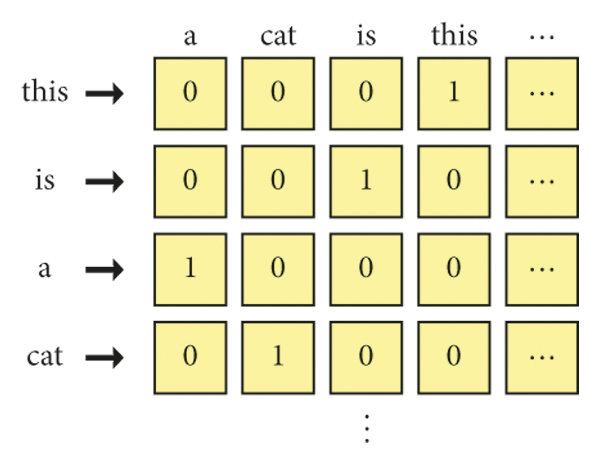
\includegraphics[scale=1.5]{assets/illustration_word_embedding.png}
      \caption{Ilustrasi \emph{Word Embedding}~\citep{Khan2021}}
      \label{fig:illustration_word_embedding}
\end{figure}

\emph{Word2Vec} merupakan salah satu bentuk implementasi dari \emph{Word Embedding} yang diajukan oleh
\citet{Mikolov2013} untuk mempelajari ekspresi dari sebuah kata termasuk juga arti
dan konteks dari kata tersebut~\citep{Jang2019}. \emph{Word2Vec} mampu memproses teks yang tidak
terstruktur dari korpus dan menghasilkan vektor sebagai keluaran dari korpus
tersebut~\citep{Nawangsari2019}. Setiap kata dari korpus dipetakan ke vektor yang berisi nilai
riil. Dengan mengubah kata menjadi vektor, kata yang memiliki makna yang sama akan direpresentasikan
berdekatan~\citep{Khattak2019}, kemiripan kata tersebut di hitung menggunakan \emph{cosine similarity}
dari vektor kata tersebut~\citep{Jang2019}. Arsitektur dari \emph{Word2Vec} ada dua yang pertama adalah \emph{Continous-Bag-Of-Words}
(CBOW) dan \emph{Skip-Gram}~\citep{Khattak2019}.

\begin{itemize}
      \item \emph{\bfseries Continous Bag Of Words} (CBOW)\\
      \emph{Continous Bag Of Words} adalah arsitektur dari \emph{Word2Vec} yang mana kata yang
      berada di sekitar kata target digunakan untuk memprediksi kata target tersebut. Prinsip
      dasar dari CBOW ini adalah memprediksi kata yang muncul berdasarkan kata
tetangga~\citep{Jang2019}. Arsitektur dari CBOW dapat diilustrasikan dengan Gambar~\ref{fig:cbow_Word2Vec}.

      \begin{figure}[H]
            \centering
            \includegraphics[scale=0.7]{assets/cbow_Word2Vec.jpg}
            \caption{Arsitektur \emph{CBOW}~\citep{Jang2019}}
            \label{fig:cbow_Word2Vec}
      \end{figure}

      \item \emph{\bfseries Continous Skip Gram}\\
      \emph{Continous Skip Gram} adalah arsitektur dari \emph{Word2Vec} merupakan kebalikan dari
      \emph{CBOW} yang mana satu kata digunakan untuk memprediksi kata sekitar. Prinsip dasar dari
      \emph{Skip-Gram} ini adalah memprediksi kata tetangga yang ada disekitar kata
      tersebut~\citep{Jang2019}. Arsitektur dari \emph{Skip-Gram} dapat diilustrasikan dengan
Gambar~\ref{fig:skip_gram_Word2Vec}.

      \begin{figure}[H]
            \centering
            \includegraphics[scale=0.7]{assets/skipgram_Word2Vec.jpg}
            \caption{Arsitektur \emph{Skip Gram}~\citep{Jang2019}}
            \label{fig:skip_gram_Word2Vec}
      \end{figure}
      
\end{itemize}

\subsection{\emph{Artificial Neural Network}}
\emph{Artificial Neural Network} (ANN) adalah pendekatan untuk memungkinkan mesin atau komputer
belajar yang terinspirasi dari cara manusia dan hewan belajar. ANN mempelajari sesuatu dengan cara
melakukan ribuan iterasi pembelajaran untuk memprediksi sesuatu berdasarkan hasil dari pembelajaran
tersebut. ANN terdiri dari beberapa lapisan simpul yang mirip dengan neuron pada otak manusia. Setiap
hasil dari lapisan simpul tersebut digunakan sebagai masukan untuk lapisan simpul selanjutnya~\citep{Desai2021}
seperti pada Gambar~\ref{fig:ann_illustration}.

ANN terdiri dari 3 lapisan \emph{(layer)}, lapisan yang pertama adalah lapisan masukan, lapisan kedua
adalah lapisan tersembunyi \emph{(hidden layer)}, dan yang ketiga adalah lapisan keluaran. Setiap lapisan
tersebut terdiri dari beberapa simpul \emph{(node)} yang terhubung ke simpul lainnya, setiap simpul
tersebut memiliki nilai ambang \emph{(Threshold)} dan nilai bobot \emph{(Weight)}.

Ketika lapisan masukan sudah ditentukan maka bobot akan mulai diinisialisasikan, kegunaan
dari bobot ini adalah untuk menentukan seberapa penting sebuah variabel dari masukan sebelumnya, dengan
nilai bobot yang besar akan mempengaruhi secara signifikan terhadap keluaran jika dibandingkan dengan
nilai masukan lainnya.


\begin{figure}[H]
      \centering
      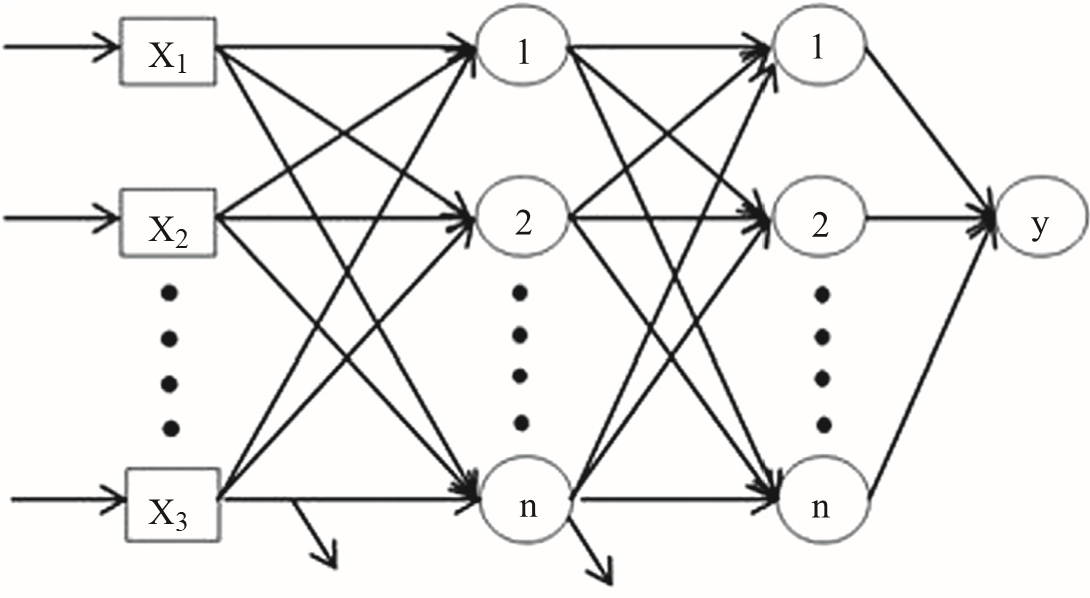
\includegraphics[scale=1]{assets/artificial_neural_network_structure.png}
      \caption{Ilustrasi ANN~\citep{Sairamya2019}}
      \label{fig:ann_illustration}
\end{figure}

\subsection{\emph{Convolutional Neural Network}}\label{CNN}
\emph{Convolutional Neural Network} (CNN) adalah \emph{feedforward neural network} yang umumnya
digunakan pada bidang \emph{computer vision}. Pendekatan CNN terinspirasi dari bagaimana cara kerja
otak manusia, dan hewan dalam mengenali gambar~\citep{Zhang2018}. Tidak seperti ANN yang lain CNN memiliki
kemampuan yang unik yaitu dapat menggabungkan ekstraksi fitur dan klasifikasi dalam satu pembelajaran
dan mengurangi keperluan untuk mengekstraksi fitur secara manual~\citep{Kiranyaz2019}. Karena hasil yang baik pada CNN
dalam pengenalan gambar, dan banyak digunakan sebagai metode klasifikasi dibarengi dengan suksesnya
klasifikasi \emph{ImageNet} dengan \emph{ConvNets} dengan landasan tersebut CNN juga dapat diaplikasikan pada
bidang analisis sentimen. Untuk menerapkan CNN pada bidang analisis sentimen maka diperlukan
penyesuaian data yang diberikan pada CNN agar dapat memahami data selain gambar dengan baik. Dalam
bidang pemrosesan bahasa alami penerapan CNN biasanya menggunakan teks yang sudah di vektorisasi sebagai
masukan yang akan diambil fiturnya dan fitur tersebut digunakan sebagai masukan pada lapisan \emph{convolution}.
Setiap simpul dari lapisan \emph{convolution} menyesuaikan dengan \emph{convolution kernel}
yang berfungsi menggabungkan masukan dari lapisan sebelumnya dengan beberapa bobot dan beberapa output
fitur untuk dijadikan masukan ke lapisan berikutnya~\citep{Wu2019}. CNN umumnya memiliki 3 lapisan
utama yaitu \emph{Convolution Layer}, \emph{Pooling Layer}, dan \emph{Fully Connected Layer}.

\begin{itemize}
      \item \emph{\bfseries Convolution Layer}\\ 
      \emph{Convolution Layer} adalah proses dimana masukan matriks dilakukan operasi konvolusi dengan
      filter yang memiliki ukuran lebih kecil dari masukan matriks untuk diekstraksi fiturnya.
      Dikarenakan ukuran filter lebih kecil dari masukan matriks setiap filter akan bergerak ke
      seluruh bagian dari masukan matriks dengan melakukan operasi konvolusi pada filter~\citep{Abdurrahman2020}.
      keluaran dari hasil operasi konvolusi akan diaplikasikan fungsi aktivasi \emph{non-linear} pada keluaran. Fungsi aktivasi
      yang digunakan pada \emph{Convolution Layer} adalah \emph{ReLU} dikarenakan
      \emph{ReLU} dapat mempercepat pembelajaran~\citep{Li2021}

      \item \emph{\bfseries Pooling Layer}\\
      \emph{Pooling Layer} atau dapat disebut juga dengan \emph{non-linear down-sampling} yang berfungsi
      untuk mereduksi dimensi dan mengurangi jumlah parameter dari hasil dari lapisan \emph{convolution}
      agar mengurangi biaya komputasi dan kalkulasi, dan untuk mengurangi \emph{overfitting} agar
      akurasi dari pengujian semakin dekat dengan akurasi latih~\citep{Wu2019}. Terdapat dua cara
      untuk melakukan \emph{pooling} yang pertama adalah \emph{Max Pooling} dan yang kedua adalah
      \emph{Average Pooling} tapi yang paling sering dipakai adalah \emph{Max Pooling} dikarenakan
      \emph{Max Pooling} dapat mempercepat konvergensi, mengambil fitur yang unggul, dan meningkatkan
      generalisasi~\citep{Chen2020}. Ilustrasi dari \emph{Max Pooling} dapat dilihat pada
      Gambar~\ref{fig:1d_max_pooling}

      \begin{figure}[H]
            \centering
            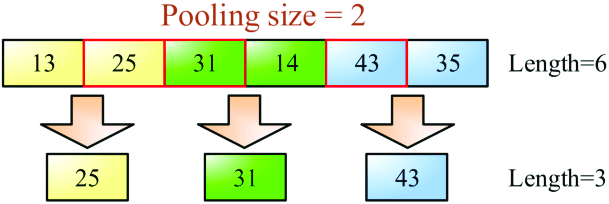
\includegraphics[scale=0.5]{assets/1d_max_pooling.png}
            \caption{Ilustrasi dari \emph{Max Pooling}~\citep{Kuo2018}}
            \label{fig:1d_max_pooling}
      \end{figure}

      \item \emph{\bfseries Fully Connected Layer}\\
      \emph{Fully Connected Layer} menerima vektor fitur sebagai masukan dan menggunakannya
      untuk mengklasifikasikan kalimat, dalam lapisan ini akan diaplikasikan regulasi untuk
      mengurangi \emph{overfitting}~\citep{Abdurrahman2020}. \emph{Fully Connected Layer} berfungsi
      untuk memastikan setiap \emph{neuron} dalam lapisan sebelumnya terkoneksi dengan \emph{neuron}
      pada lapisan berikutnya~\citep{Pandey2022}. Pada lapisan ini umumnya menggunakan aktivasi
      fungsi \emph{Softmax} untuk klasifikasi yang lebih dari dua label dan \emph{Sigmoid} untuk
      klasifikasi dua label~\citep{Li2021}.
\end{itemize}

\emph{Softmax} biasa disebut juga \emph{softargmax} berfungsi untuk mengubah sebuah vektor $K$ yang
bernilai rill menjadi vektor $K$ yang bernilai rill dalam bentuk distribusi probabilitas dari $K$
kemungkinan yang akan terjadi dan apa bila nilainya dijumlahkan akan bernilai 1~\citep{Wood2019}.

\begin{equation}\label{eq:softmax}
      \sigma(z_i) = \frac{e^{z_{i}}}{\sum_{j=1}^K e^{z_{j}}}
\end{equation}

Keterangan:
\begin{itemize}
      \item $z_i = vektor \ masukan$
      \item $K = jumlah \ kelas$
\end{itemize}

\emph{Rectified Linear Unit (ReLu)} adalah fungsi aktivasi yang umumnya digunakan pada jaringan
syaraf tiruan untuk mendapatkan nilai aktivasi yang sesuai pada setiap \emph{neuron}. Alasan penggunaan
\emph{ReLU} daripada fungsi aktivasi yang lain adalah \emph{ReLU} dapat mempercepat waktu latih dari
jaringan syaraf tiruan dikarenakan hasil turunan dari \emph{ReLU} adalah 1 untuk masukan yang
bernilai positif dan 0 untuk masukan yang negatif dengan kata lain \emph{neuron} hanya akan
diaktifkan ketika nilainya bernilai positif~\citep{Li2021}. Persamaan dari \emph{ReLU} dapat dilihat pada persamaan
\ref{eq:relu} dan \ref{eq:relu2} untuk grafik \emph{ReLU} dapat di lihat di Gambar~\ref{fig:relu}

\begin{figure}[H]
      \centering
      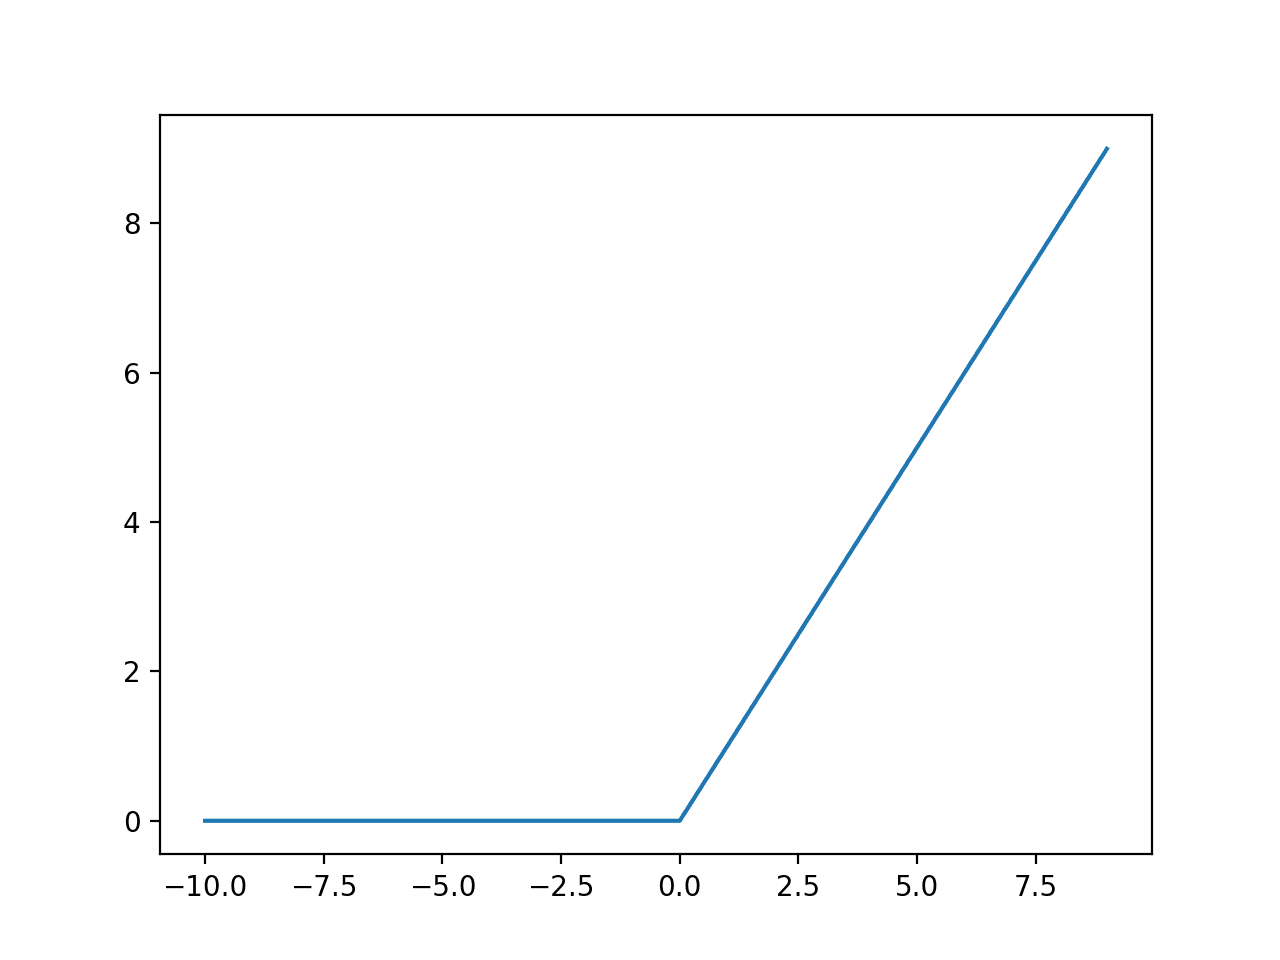
\includegraphics[scale=0.2]{assets/rectified_linear_unit.png}
      \caption{Contoh Grafik dari \emph{ReLU}}
      \label{fig:relu}
\end{figure}

\begin{equation}\label{eq:relu}
      ReLU(x) = \max(0, x)
\end{equation}


\begin{equation}\label{eq:relu2}
      ReLU(x) = \begin{cases}
            0, & \text{if } x < 1  \\
            x, & \text{if } x >= 0 \\
      \end{cases}
\end{equation}

Keterangan:
\begin{itemize}
      \item $x = nilai \ masukan$
\end{itemize}

CNN juga memiliki beberapa parameter yang disebut \emph{hyperparameter}, seperti berapa jumlah filter
(\emph{number of filter}), ukuran filter (\emph{filter size}), \emph{dropout} dan sebagainya.
Peningkatan performa pada CNN akan terjadi apabila nilai dari parameter tersebut
dioptimalkan~\citep{Akhter2020}.

\subsection{\emph{Confusion Matrix}}\label{Confusion Matrix}
\emph{Confusion Matrix} adalah cara untuk mengukur performa dari sistem klasifikasi berdasarkan
data yang dilatih dan data yang diuji. \emph{Confusion Matrix} berbentuk matriks dua dimensi,
dimensi pertama adalah label atau kelas yang asli, dan dimensi yang lain adalah label atau kelas
hasil dari sistem klasifikasi~\citep{Deng2016}. Ada 4 nilai yang dihasilkan dari \emph{Confusion Matrix},
diantaranya \emph{True Positive (TP)}, \emph{False Positive (FP)}, \emph{False Negative (FN)}, dan
\emph{True Negative (TN)} seperti pada Gambar~\ref{fig:ilustrasi_confusion_matrix}.

\begin{itemize}
      \item \emph{\bfseries True Positive (TP)} adalah nilai hasil prediksi positif dan nilai sebenarnya positif.
      \item \emph{\bfseries True Negative (TN)} adalah nilai hasil prediksi negatif dan nilai sebenarnya negatif.
      \item \emph{\bfseries False Positive (FP)} adalah nilai hasil prediksi positif dan nilai sebenarnya negatif.
      \item \emph{\bfseries False Negative (FN)} adalah nilai hasil prediksi negative dan nilai sebenarnya positif.
\end{itemize}

\begin{figure}[H]
      \centering
      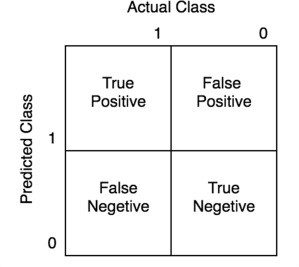
\includegraphics[scale=1]{assets/confusion_matrix.jpg}
      \caption{Ilustrasi \emph{Confusion Matrix}~\citep{Sharma2022}}
      \label{fig:ilustrasi_confusion_matrix}
\end{figure}


Hasil dari nilai \emph{confusion matrix} tadi dapat dijadikan beberapa metrik yaitu \emph{Precision},
\emph{Sensitivity (Recall)}, \emph{F-Measure (F1-Score)}, dan \emph{Accuracy}.


\begin{itemize}
      \item \emph{\bfseries Precision}\\
      \emph{Precision} adalah metrik yang digunakan untuk mengukur berapa banyak prediksi yang benar
      dalam total prediksi yang dilakukan. Cara penghitungan \emph{Precision} adalah prediksi yang
      benar dibagi total prediksi yang telah dilakukan. \emph{Precision} dapat dihitung menggunakan
      persamaan~\ref{eq:Precision}.

      \begin{equation}\label{eq:Precision}
            Precision = \frac{TP}{TP + FP}
      \end{equation}

      \item \emph{\bfseries \emph{Sensitivity (Recall)}}\\
      \emph{Sensitivity (Recall)} adalah metrik yang digunakan untuk mengukur berapa banyak prediksi yang
      benar dalam jumlah kelas atau label yang ada. Nilai tertinggi dalam \emph{Sensitivity (Recall)}
      adalah 1,0 dan nilai yang terendah adalah 0,0. \emph{Sensitivity (Recall)} dapat dihitung menggunakan
      persamaan~\ref{eq:Sensitivity_recall}.

      \begin{equation}\label{eq:Sensitivity_recall}
            Sensitivity = \frac{TP}{TP + FN}
      \end{equation}

      \item \emph{\bfseries F-Measure (F1-score)}\\
      \emph{F-Measure (F1-Score)} adalah rata-rata harmonik dari \emph{Precision} dan \emph{Sensitivity (Recall)}, berguna
      untuk menyeimbangkan nilai dari \emph{Precision} dan \emph{Sensitivity (Recall)} nilai \emph{F-Measure (F1-Score)} akan
      tinggi jika nilai dari \emph{Precision} dan \emph{Sensitivity (Recall)} tinggi dan akan rendah jika nilai dari
      \emph{Precision} dan \emph{Sensitivity (Recall)} rendah. \emph{F-Measure (F1-Score)} dapat dihitung menggunakan
      persamaan~\ref{eq:f_score_f_measure}.

      \begin{equation}\label{eq:f_score_f_measure}
            F-Measure = 2 \times \frac{Recall \times Precision}{Recall + Precision}
      \end{equation}

      \item \emph{\bfseries Accuracy}\\
      \emph{Accuracy} atau akurasi merupakan salah satu metrik yang biasa digunakan untuk mengevaluasi
      kinerja model pada semua kelas atau label. Metrik ini berguna ketika kelas memiliki bobot yang
      setara dengan kelas yang lainnya. Cara penghitungan metrik adalah rasio antara jumlah prediksi
      yang benar dengan jumlah total prediksi. \emph{Accuracy} dapat dihitung menggunakan
      persamaan~\ref{eq:Accuracy}.

      \begin{equation}\label{eq:Accuracy}
            Accuracy = \frac{(TP + TN)}{(TP + FP + TN + FN)}
      \end{equation}

\end{itemize}

\subsection{\emph{Rational Unified Process} (RUP)}
\emph{Rational Unified Process} (RUP) adalah salah satu metode pengembangan perangkat lunak yang
menerapkan konsep orientasi objek dan umumnya digunakan untuk pengembangan aplikasi
berbasis \emph{web}. Tujuan dari RUP adalah untuk memastikan perangkat lunak yang dikembangkan
berkualitas tinggi yang memenuhi ekspektasi dari pengguna. Dalam skala besar RUP bersifat bersambung,
namun dalam skala kecil RUP bersifat iteratif dan bertahap untuk perilisan
\emph{software}-nya~\citep{anwar2014review}. RUP ditemukan dan dikembangkan oleh
Rational\textregistered~Software. RUP terdiri dari empat fase bersifat iteratif yaitu Fase Insepsi,
Fase Elaborasi, Fase Konstruksi dan Fase Transisi seluruh fase tersebut dapat diilustrasikan pada Gambar~\ref{fig:rup}.

\begin{itemize}
      \item \emph{\bfseries Fase Insepsi}\\ 
      Fase Insepsi terdiri dari mendifinisikan kasus bisnis,
      membatasi ruang lingkup proyek, menentukan kebutuhan dari perangkat lunak dan mendesain perangkat
      lunak sesuai dengan kasus bisnis.

      \item \emph{\bfseries Fase Elaborasi}\\
      Fase Elaborasi adalah menganalisa berbagai persyaratan dan resiko dalam pengembangan perangkat
      lunak. Elaborasi juga memastikan arsitektur, kebutuhan, dan perencanaan stabil dan tidak banyak
      yang diubah ketika ada perubahan.

      \item \emph{\bfseries Fase Konstruksi}\\
      Fase Konstruksi adalah fase dimana perangkat lunak mulai
      diimplementasikan dalam bentuk kode program sesuai dengan kebutuhan bisnis dan kebutuhan dari
      perangkat lunak tersebut. Setiap kode program yang sudah diimplementasikan akan diuji.

      \item \emph{\bfseries Fase Transisi}\\
      Fase Transisi adalah fase perangkat lunak mulai disebarkan pada pengguna, apabila perangkat
      lunak masih memiliki masalah atau terdapat ketidaksesuaian dengan yang diekspektasikan oleh
      pengguna maka program akan dikembangkan lagi dan dirilis ulang dengan penundaan pada penambahan
      fitur atau perbaikan masalah.

\end{itemize}

\begin{figure}[H]
      \centering
      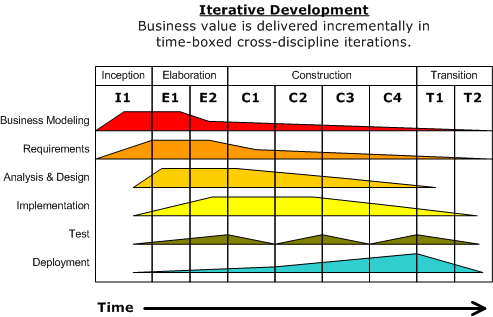
\includegraphics[scale=0.7]{assets/rup.png}
      \caption{Fase RUP}
      \label{fig:rup}
\end{figure}

\section{Pustaka (\emph{Library \& Framework}) yang Digunakan}

\begin{itemize}
      {\bfseries \item \emph{Tensorflow}}\\
      Dilansir dari website resminya \emph{Tensorflow} adalah \emph{platform} ujung-ke-ujung (\emph{end-to-end})
      dengan sumber terbuka (\emph{open source}) untuk membuat model pembelajaran
      mesin (\emph{machine learning}). \emph{Tensorflow} mempermudah pemula dan ahli untuk membuat model
      pembelajaran mesin (\emph{machine learning})~\citep{tensorflow2015-whitepaper}. Ada 2 cara yang
      dapat dilakukan untuk menyebarkan model machine learning pada aplikasi \emph{mobile} menggunakan
      \emph{Tensorflow} yaitu \emph{Tensorflow Lite} dan \emph{Tensorflow Serving}.

      \begin{itemize}
            {\bfseries \item \emph{Tensorflow Lite}} Dilansir dari website resminya \emph{Tensorflow Lite}
            adalah pustaka (\emph{library}) untuk menyebarkan (\emph{deploy}) model \emph{machine learning} pada \emph{mobile}
            (\emph{handphone}), \emph{microcontroller}, dan peranti yang memiliki sumber daya yang
            sedikit~\citep{tensorflow2015-whitepaper}.

            {\bfseries \item \emph{Tensorflow Serving}} Dilansir dari website resminya \emph{Tensorflow Serving}
            adalah cara yang fleksibel, berperforma tinggi untuk menyebarkan model \emph{machine learning}
            pada \emph{server}~\citep{tensorflow2015-whitepaper}.
      \end{itemize}

      {\bfseries \item \emph{Scikit-Learn}}\\
      Dilansir dari website resminya \emph{Scikit-Learn} adalah pustaka (\emph{Library}) untuk bahasa pemrograman
      python yang menyediakan banyak alat untuk melakukan pembelajaran mesin (\emph{machine-learning}) secara
      diawasi (\emph{supervised}) dan tidak diawasi (\emph{unsupervised})~\citep{scikit-learn}. Fitur-fitur
      yang ada di \emph{scikit-learn} yaitu klasifikasi, regresi, klusterisasi, reduksi dimensi,
      pemilihan model, dan praproses.

      {\bfseries \item \emph{Gensim}}\\
      Dilansir dari website resminya \emph{Gensim} atau \emph{Generate Similar} adalah pustaka untuk bahasa
      pemrograman python yang berfungsi untuk merepresentasikan dokumen sebagai vektor semantik seefisien mungkin dan semudah
      mungkin. \emph{Gensim} didesain untuk memproses data yang tidak terstruktur atau \emph{(`Plain Text')}
      menggunakan algoritma pembelajaran mesin yang tidak diawasi~\citep{rehurek_lrec}. Algoritma yang
      tersedia pada Gensim adalah \emph{Word2Vec}, \emph{FastText} dan sebagainya.

      {\bfseries \item \emph{Google-Play-Scraper}}\\
      Dilansri dari website github dan pypi \emph{Google-Play-Scraper} adalah pustaka untuk bahasa pemrograman
      python yang berfungsi untuk memudahkan \emph{web crawling} pada website \emph{Google Play Review}.

      {\bfseries \item Sastrawi}\\
      Dilasir dari website github dan pypi Sastrawi adalah pustaka untuk bahasa pemrograman python yang
      berfungsi untuk melakukan \emph{stemming} dan menghilangkan \emph{stopword} pada bahasa indonesia.

\end{itemize}

\section{Penelitian Yang Relevan}
\citet{Sharma2020} menggunakan CNN dan \emph{pre-trained Word2Vec} untuk analisis sentimen pada
dataset IMDb \emph{movie review} berjumlah 5331 berlabel positif dan 5331 berlabel negatif dan di
praproses dengan cara mengubah \emph{multilingual} data menjadi Bahasa Inggris, \emph{Tokenize} pada
setiap spasi, menghapus pungtuasi, menghapus stoword, menghapus kata dengan panjang \leq~1 karakter,
dan teks diubah menjadi \emph{lowercase} menghasilkan model dengan akurasi sebesar 99,07\% pada data
latih dan 82,19\% pada data uji. Dari penelitian ini dapat disimpulkan bahwa CNN dan \emph{Word2Vec}
sangat efektif dan efisien untuk analisis sentimen.

\citet{Dong2020} menggunakan CNN untuk analisis sentimen perkalimat pada dataset saham yang sudah
di praproses dengan cara menghilangkan angka dan karakter spesial, \emph{stemming}, \emph{casefolding},
dan \emph{tokenize}. Menghasilkan model dengan akurasi 98,1\% dibandingkan dengan \emph{SVM (Support Vector Machine)} yang
memiliki akurasi 90\% dan \emph{Random Forest} memiliki akurasi 93\%. Dari hasil penelitian tersebut
dapat diambil kesimpulan bahwa CNN melebihi akurasi dari \emph{SVM (Support Vector Machine)} dan
\emph{Random Forest}.

\citet{Smetanin2019} menggunakan CNN dan \emph{pre-trained Word2Vec} yang dilatih dari 5.5 juta \emph{review}
untuk analisis sentimen pada produk \emph{review} dalam bahasa Rusia dari kategori `Women's Clothes and Accessories'
berjumlah 821 ribu \emph{review} yang dilabel secara otomatis dan di praproses dengan cara \emph{lowercase},
mengubah emotikon menjadi \emph{emotional tag}, dan normalisasi teks. Mendapatkan hasil dengan
\emph{Precision} 75,63\%, \emph{Recall} 75,31\% dan \emph{F1-score} 75,45\% yang kemudian dibandingkan
dengan algoritma pembelajaran mesin \emph{Multinomial Naive Bayes} dengan hasil \emph{Precision} 74,47\%,
\emph{Recall} 73,79\% dan \emph{F1-score} 73,90\%. Dari penelitian ini dapat diambil kesimpulan
bahwa CNN dan \emph{Word2Vec} dapat melebihi kinerja dari \emph{Multinomial Naive Bayes}.

\citet{Amanatidis2019} menggunakan CNN dan \emph{Word2Vec} yang sudah dilatih terlebih dahulu dengan
menggunakan dataset IMDb \emph{movie review} untuk melakukan analisis sentimen pada data \emph{review}
TripAdvisor, setiap \emph{review} dipraproses dengan cara \emph{lowercase}, menghapus pungtuasi,
mempadding \emph{review}, dan memotong \emph{review} yang lebih dari 1000 kata. Hasil dari CNN yang di
latih dengan menggunakan dataset IMDb \emph{movie review} menghasilkan akurasi 88,85\%. Dari hasil penelitian
tersebut dapat disimpulkan bahwa CNN dan \emph{Word2Vec} dapat dengan mudah menghasilkan akurasi 88,85\%.

\citet{Aldiansyah2019} menggunakan CNN dan \emph{Word2Vec} untuk analisis sentimen pada opini publik
untuk jaringan 4G Smartfren yang berjumlah 1120 kicauan yang dilabeli secara manual menjadi dua label
yang berjumlah 560 positif dan 560 negatif. Kicauan tersebut dipraproses dengan cara \emph{casefolding},
\emph{tokenization}, penghapusan pungtuasi, pengahapusan \emph{stopword}, dan \emph{stemming} menghasilkan
model dengan akurasi 88,21\%.

\section{Kesimpulan}
Bab ini sudah memberikan landasan teori dari beberapa literatur dan juga memberikan penjelasan dari
penelitian lain yang relevan dengan penelitian yang dilakukan yaitu analisis sentimen menggunakan CNN\@.
\pagestyle{fancy}
\fancypagestyle{plain}{}
\cfoot{\Roman{chapter}-\arabic{page}}
\rhead{}
\setcounter{page}{1}
\chapter{METODOLOGI PENELITIAN}

\section{Pendahuluan}
Pada bab ini akan menjabarkan metodologi penelitian serta manajemen proyek penelitian yang akan
diimplementasikan pada penelitian ini. Tahapan penelitian akan dijadikan sebagai landasan untuk
setiap fase pengembangan perangkat lunak dan memberikan sebuah solusi berdasarkan rumusan masalah
untuk mencapai tujuan penelitian.

\section{Pengumpulan Data}~\label{sec:pengumpulan_data}
Dalam bagian ini akan diuraikan bagaimana tahapan penulis dalam melakukan pengumpulan data yang akan
digunakan dalam penelitian.

\subsection{Jenis Data}
Data yang digunakan dalam penelitian ini adalah jenis data primer. Data primer adalah data yang
diambil dari sumbernya langsung melalui sumber aslinya tanpa perantara. Jumlah data primer direncanakan
sebanyak 6.000 \emph{review}, dengan 3.000 berlabel positif dan 3.000 \emph{review} berlabel
negatif. Data tersebut akan digunakan untuk melatih CNN dalam melakukan analisis sentimen.

\subsection{Sumber Data}
Data primer yang akan digunakan untuk melaksanakan penelitian ini diperoleh dari \emph{review}
aplikasi gojek, grab, dan maxim yang ada di \emph{Google Play Store}. Data \emph{review} telah
dilabeli menjadi dua kelas, yaitu positif dan negatif secara otomatis berdasarkan skor dari
\emph{review} yang ada di \emph{Google Play Store} dengan ketentuan 1 adalah label negatif dan 5
adalah label positif~\citep{Akbar2022},~\citep{Smetanin2019},~\citep{Amanatidis2019}.\newpage


\pagestyle{fancy}
\fancypagestyle{plain}{}
\rhead{\Roman{chapter}-\arabic{page}}
\cfoot{}

\subsection{Metode Pengumpulan Data}
Pengumpulan data primer dilakukan dengan cara mengunduh yaitu \emph{crawling} di website
\emph{Google Play Store} dengan bantuan pustaka (\emph{library}) \emph{google-play-scraper}. Data
dikumpulkan dari \emph{review} 3 aplikasi angkutan online yaitu gojek, grab, dan maxim dengan kriteria
jumlah kata dalam kalimat minimal 11 kata. Masing-masing review dari 3 aplikasi tersebut diambil
1000 dengan skor 1 dan 1000 dengan skor 5.

\subsection{Contoh Data Sentimen}
Dalam bagian ini akan ditampilkan contoh data sentimen yang akan digunakan dalam penelitian ini
dalam bentuk tabel dapat dilihat pada Tabel~\ref{tab:contoh_data_sentimen}.

\begin{table}[H]
  \centering
  \caption{Contoh Data Sentimen}
  \label{tab:contoh_data_sentimen}
  \begin{tabularx}{\columnwidth}{|X|X|l|}
    \hline
    reviewId                             & content                                                                                                                                                                          & label   \\ \hline
    d4e7736d-f5ea-4c8e-af74-198266968a76 & Gk jelas aplikasi ini gk kaya punya sebelah lokasi tujuan udh di tulis yg keluar alamat lain.masa order blm ada tujuanya udh masuk kn bikin stres ampe emosi gw. Hancur pokoknya & Negatif \\ \hline
    a5a355f8-a208-44d6-8a7f-f255139d20fa & Gda LG kecuali gojek...top pokok y                                                                                                                                               & Positif \\ \hline
    3ad826e8-7f10-4854-9d16-3dd90eefbada & cpt banget                                                                                                                                                                       & Positif \\ \hline
    c7ded523-ead6-4bc3-aa2f-69b226e52d02 & Mending gojek aja                                                                                                                                                                & Negatif \\ \hline
  \end{tabularx}
\end{table}

Dan untuk jumlah sentimen yang bernilai positif dan negatif dapat dilihat pada Gambar~\ref{fig:bar_pos_neg}.
\begin{figure}[H]
  \centering
  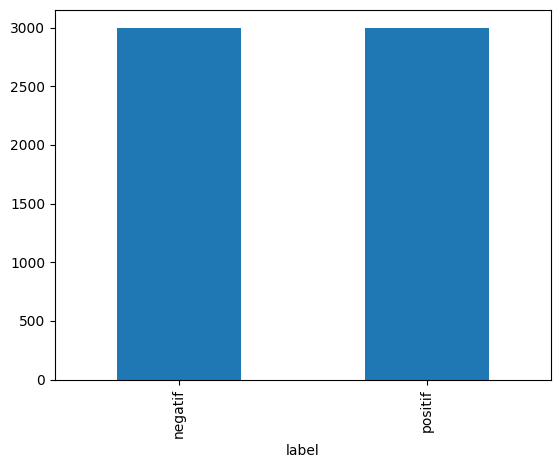
\includegraphics[scale=0.5]{assets/bar_pos_neg.png}
  \caption{Jumlah Sentimen Positif dan Negatif}
  \label{fig:bar_pos_neg}
\end{figure}

\section{Tahapan Penelitian}
Untuk mengetahui kinerja dari \emph{Convolutional Neural Network} pada klasifikasi sentimen, maka
penelitian ini dilakukan dengan tahapan pada penelitian seperti pada Gambar~\ref{fig:diagram_tahapan_penelitian}.

\begin{figure}[H]
  \centering
  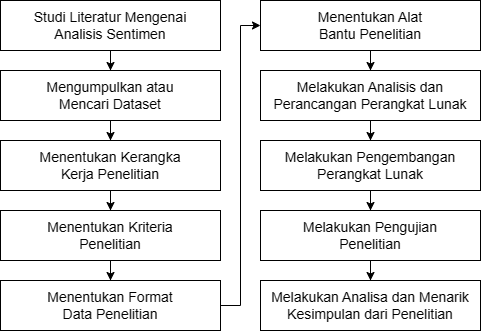
\includegraphics[scale=0.59]{assets/diagram_tahapan_penelitian.png}
  \caption{Diagram Tahapan Penelitian}
  \label{fig:diagram_tahapan_penelitian}
\end{figure}

\subsection{Studi Literatur Mengenai Analisis Sentimen}
Dalam tahapan penelitian ini penulis melakukan studi literatur mengenai analisis sentimen. Penulis
menganalisa, memahami, mengumpulkan semua sumber yang berkaitan dengan analisis sentimen dengan
tujuan untuk mendapatkan landasan dalam penelitian yang dilakukan. Dengan didapatkannya landasan yang
memiliki relevansi pada permasalahan yang diteliti diharapkan nantinya dapat membantu dalam proses
penelitian.

\subsection{Mengumpulkan / Mencari Dataset}
Dalam tahapan penelitian ini penulis melakukan pengumpulan data dengan dua tujuan yang pertama adalah
untuk melatih model CNN dalam analisis sentimen, dan yang terakhir adalah untuk mempermudah penanganan
bahasa gaul. CNN dengan model yang baik dapat diperoleh dengan cara melatih CNN menggunakan banyak
data. Semakin banyak data yang dapat digunakan untuk melatih CNN maka model dari CNN akan menjadi
lebih akurat.

\subsection{Kerangka Kerja Penelitian}
Analisis sentimen dalam penelitian ini akan dijalankan beberapa tahapan, yaitu studi literatur
untuk memahami permasalahan yang diteliti, persiapan data agar dapat diimplementasikan kedalam program,
pra-pengolahan data, proses latih data menggunakan metode CNN, analisis hasil, dan penarikan kesimpulan.
Kerangka kerja penelitian dapat dilihat pada Gambar~\ref{fig:kerangka_kerja_penelitian}.

\begin{figure}[H]
  \centering
  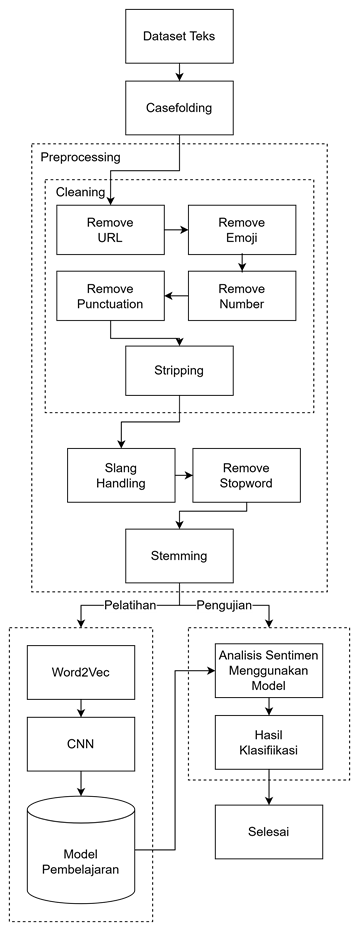
\includegraphics[width=\textwidth, height=15cm, keepaspectratio]{assets/kerangka_kerja_penelitian.png}
  \caption{Kerangka Kerja Penelitian}
  \label{fig:kerangka_kerja_penelitian}
\end{figure}

Berdasarkan kerangka kerja pada Gambar~\ref{fig:kerangka_kerja_penelitian}, analisis sentimen menggunakan
CNN memiliki tahapan sebagai berikut.

\begin{enumerate}
  {\bfseries \item Praproses Teks}\\
  Langkah pertama yang dilakukan dalam penelitian ini adalah praproses teks. Pada tahapan ini teks
  diubah ke huruf kecil (\emph{casefolding}), teks akan dihilangkan \emph{URL} (\emph{URL Removal}),
  dihilangkan emotikon, dihilangkan angka, dihilangkan tanda baca. Dilanjutkan dengan penanganan
  bahasa gaul, dihilangkan \emph{stopword}, diubah menjadi kata dasar atau \emph{stemming}, dan \emph{tokenizing}.
  Untuk penjelasan yang lebih detail pada langkah-langkah praproses dapat dilihat pada~\autoref{Praproses}.

  \begin{enumerate}
    {\bfseries \item \emph{Casefolding}}\\
    Langkah pertama dalam praproses adalah casefolding, casefolding merupakan teknik merubah semua
    huruf didalam teks menjadi seragam umumnya adalah huruf kecil. Contoh kalimat sebelum dilakukan
    \emph{casefolding} dan yang sudah dilakukan \emph{casefolding} dapat dilihat pada Tabel~\ref{tab:contoh_casefolding}

    \begin{table}[H]
      \centering
      \caption{Contoh \emph{Casefolding}}
      \label{tab:contoh_casefolding}
      \begin{tabularx}{\columnwidth}{|X|X|}
        \hline
        content                                                                                                                                                                                      & lowercased                                                                                                                                                                                   \\ \hline
        {\bfseries Gk} jelas aplikasi ini gk kaya punya sebelah lokasi tujuan udh di tulis yg keluar alamat lain.masa order blm ada tujuanya udh masuk kn bikin stres ampe emosi gw. Hancur pokoknya & {\bfseries gk} jelas aplikasi ini gk kaya punya sebelah lokasi tujuan udh di tulis yg keluar alamat lain.masa order blm ada tujuanya udh masuk kn bikin stres ampe emosi gw. hancur pokoknya \\ \hline
        {\bfseries Gda LG} kecuali gojek...top pokok y                                                                                                                                               & {\bfseries gda lg} kecuali gojek...top pokok y                                                                                                                                               \\ \hline
        cpt banget                                                                                                                                                                                   & cpt banget                                                                                                                                                                                   \\ \hline
        {\bfseries Mending} gojek aja                                                                                                                                                                & {\bfseries mending} gojek aja                                                                                                                                                                \\ \hline
      \end{tabularx}
    \end{table}

    {\bfseries \item \emph{Cleaning}}\\
    Langkah selanjutnya adalah pembersihan teks dari karakter yang tidak diperlukan. Langkah-langkah
    dalam tahapan \emph{cleaning} ini yaitu, \emph{Remove URL}, \emph{Remove Emoji}, \emph{Remove Number},
    \emph{Remove Punctuation}, dan \emph{Stripping} untuk penjelasan lebih detil pada tahapan cleaning
    dapat dilihat pada~\autoref{Praproses}. Contoh kalimat sebelum dilakukan \emph{cleaning} dan yang
    sudah dilakukan \emph{cleaning} dapat dilihat pada Tabel~\ref{tab:contoh_cleaning}.

    \begin{table}[H]
      \centering
      \caption{Contoh \emph{Cleaning}}
      \label{tab:contoh_cleaning}
      \begin{tabularx}{\columnwidth}{|X|X|}
        \hline
        lowercased                                                                                                                                                                       & cleaned                                                                                                                                                                          \\ \hline
        gk jelas aplikasi ini gk kaya punya sebelah lokasi tujuan udh di tulis yg keluar alamat lain.masa order blm ada tujuanya udh masuk kn bikin stres ampe emosi gw. hancur pokoknya & gk jelas aplikasi ini gk kaya punya sebelah lokasi tujuan udh di tulis yg keluar alamat lain masa order blm ada tujuanya udh masuk kn bikin stres ampe emosi gw  hancur pokoknya \\ \hline
        gda lg kecuali gojek \underline{\ldots} top pokok y                                                                                                                              & gda lg kecuali gojek top pokok y                                                                                                                                                 \\ \hline
        cpt banget                                                                                                                                                                       & cpt banget                                                                                                                                                                       \\ \hline
        mending gojek aja                                                                                                                                                                & mending gojek aja                                                                                                                                                                \\ \hline
      \end{tabularx}
    \end{table}

    {\bfseries \item \emph{Slang Handling}}\\
    Langkah selanjutnya adalah mengubah kata gaul menjadi kata formalnya dengan menggunakan kamus alay
    hasil dari penelitian \citet{Aliyah2018}. Contoh kalimat sebelum dilakukan \emph{slang handling}
    dan yang sudah dilakukan \emph{slang handling} dapat dilihat pada Tabel~\ref{tab:contoh_slang_handling}.

    \begin{table}[H]
      \centering
      \caption{Contoh \emph{Slang Handling}}
      \label{tab:contoh_slang_handling}
      \begin{tabularx}{\columnwidth}{|X|X|}
        \hline
        cleaned                                                                                                                                                                                                                                                                          & slang\_handled                                                                                                                                                                                                                                                                                       \\ \hline
        {\bfseries gk} jelas aplikasi ini {\bfseries gk kaya} punya sebelah lokasi tujuan {\bfseries udh} di tulis yg keluar alamat lain masa order {\bfseries blm} ada tujuanya {\bfseries udh} masuk {\bfseries kn} bikin stres {\bfseries ampe} emosi {\bfseries gw}  hancur pokoknya & {\bfseries enggak} jelas aplikasi ini {\bfseries enggak kayak} punya sebelah lokasi tujuan {\bfseries sudah} di tulis yang keluar alamat lain masa order {\bfseries belum} ada tujuanya {\bfseries sudah} masuk {\bfseries kan} bikin stres {\bfseries sampai} emosi {\bfseries gue} hancur pokoknya \\ \hline
        {\bfseries gda lg} kecuali gojek top pokok {\bfseries y}                                                                                                                                                                                                                         & {\bfseries enggak ada lagi} kecuali gojek top pokok {\bfseries ya}                                                                                                                                                                                                                                   \\ \hline
        {\bfseries cpt} banget                                                                                                                                                                                                                                                           & {\bfseries cepat} banget                                                                                                                                                                                                                                                                             \\ \hline
        mending gojek {\bfseries aja}                                                                                                                                                                                                                                                    & mending gojek {\bfseries saja}                                                                                                                                                                                                                                                                       \\ \hline
      \end{tabularx}
    \end{table}

    {\bfseries \item \emph{Stopword Removal}}\\
    Langkah selanjutnya adalah menghilangkan kata yang tidak memiliki makna dari kalimat, proses ini
    dilakukan dengan bantuan pustaka (\emph{library}) Sastrawi. Contoh kalimat sebelum dilakukan
    \emph{stopword removal} dan yang sudah dilakukan \emph{stopword removal} dapat dilihat
    pada Tabel~\ref{tab:contoh_stopword_removal}.

    \begin{table}[H]
      \centering
      \caption{Contoh \emph{Stopword Removal}}
      \label{tab:contoh_stopword_removal}
      \begin{tabularx}{\columnwidth}{|X|X|}
        \hline
        slang\_handled                                                                                                                                                                                                                                                                                                   & stopword\_removed                                                                                      \\ \hline
        {\bfseries enggak jelas} aplikasi {\bfseries ini enggak} kayak {\bfseries punya} sebelah lokasi tujuan {\bfseries sudah di} tulis {\bfseries yang keluar} alamat {\bfseries lain masa} order {\bfseries belum ada} tujuanya {\bfseries sudah masuk kan} bikin stres {\bfseries sampai} emosi gue hancur pokoknya & aplikasi kayak sebelah lokasi tujuan tulis alamat order tujuanya bikin stres emosi gue hancur pokoknya \\ \hline
        {\bfseries enggak ada lagi} kecuali gojek top pokok {\bfseries ya}                                                                                                                                                                                                                                               & kecuali gojek top pokok                                                                                \\ \hline
        cepat banget                                                                                                                                                                                                                                                                                                     & cepat banget                                                                                           \\ \hline
        mending gojek {\bfseries saja}                                                                                                                                                                                                                                                                                   & mending gojek                                                                                          \\ \hline
      \end{tabularx}
    \end{table}

    {\bfseries \item \emph{Stemming}}\\
    Langkah selanjutnya adalah mengubah kata yang ada didalam kalimat menjadi kata dasarnya, proses ini
    dilakukan dengan bantuan pustaka (\emph{library}) Sastrawi. Contoh
    kalimat sebelum dilakukan \emph{stemming} dan yang sudah dilakukan \emph{stemming} dapat dilihat
    pada Tabel~\ref{tab:contoh_stemming}.

    \begin{table}[H]
      \centering
      \caption{Contoh \emph{Stemming}}
      \label{tab:contoh_stemming}
      \begin{tabularx}{\columnwidth}{|X|X|}
        \hline
        stopword\_removed                                                                                                              & stemmed                                                                                                                 \\ \hline
        aplikasi kayak {\bfseries sebelah} lokasi {\bfseries tujuan} tulis alamat order tujuanya bikin stres emosi gue hancur pokoknya & aplikasi kayak {\bfseries belah} lokasi {\bfseries tuju} tulis alamat order tujuanya bikin stres emosi gue hancur pokok \\ \hline
        kecuali gojek top pokok                                                                                                        & kecuali gojek top pokok                                                                                                 \\ \hline
        cepat banget                                                                                                                   & cepat banget                                                                                                            \\ \hline
        mending gojek                                                                                                                  & mending gojek                                                                                                           \\ \hline
      \end{tabularx}
    \end{table}

    {\bfseries \item \emph{Tokenizing}}\\
    Langkah selanjutnya adalah memecah kalimat menjadi kumpulan kata, kata dipecah pada setiap spasi.
    Contoh kalimat sebelum dilakukan \emph{Tokenizing} dan yang sudah
    dilakukan \emph{Tokenizing} dapat dilihat pada Tabel~\ref{tab:contoh_tokenizing}.

    \begin{table}[H]
      \centering
      \caption{Contoh \emph{Tokenizing}}
      \label{tab:contoh_tokenizing}
      \begin{tabularx}{\columnwidth}{|X|X|}
        \hline
        stemmed                                                                                         & tokenized                                                                                                       \\ \hline
        aplikasi kayak belah lokasi tuju tulis alamat order tujuanya bikin stres emosi gue hancur pokok & [aplikasi, kayak, belah, lokasi, tuju, tulis, alamat, order, tujuanya, bikin, stres, emosi, gue, hancur, pokok] \\ \hline
        kecuali gojek top pokok                                                                         & [kecuali, gojek, top, pokok]                                                                                    \\ \hline
        cepat banget                                                                                    & [cepat, banget]                                                                                                 \\ \hline
        mending gojek                                                                                   & [mending, gojek]                                                                                                \\ \hline
      \end{tabularx}
    \end{table}
  \end{enumerate}

  {\bfseries \item Membagi Data Latih dan Data Uji}\\
  Setelah kata dijadikan token dataset akan dibagi umumnya dataset dibagi menjadi 3, data latih,
  data validasi dan data uji. Dataset berjumlah 6000 dibagi menjadi 60:20:20 ke data latih, data validasi,
  dan data uji sehingga jumlah data latih menjadi 4800 data, dan data uji menjadi 1200 data.

  {\bfseries \item \emph{Word2Vec}}\\
  \emph{Word2Vec} adalah salah satu cara untuk melakukan \emph{word embedding} yang berguna untuk
  merepresentasikan kata menjadi vektor bernilai rill~\citep{Khattak2019}. \emph{Word2Vec} yang
  digunakan pada penelitian ini adalah \emph{pre-trained Word2Vec} yang didapatkan dari \emph{website kaggle}
  \url{https://www.kaggle.com/datasets/bhimantoros/pretrained-word2vec-indonesia}.
  \emph{Word2Vec} tersebut dilatih dengan menggunakan \emph{dump} dari Wikipedia Bahasa Indonesia (\emph{latest})
  dengan parameter $vector\_size=400$ dan $window=5$.

  {\bfseries \item \emph{Word Embedding}}\\
  Tahapan selanjutnya adalah mengubah token menjadi bentuk \emph{word embedding} menggunakan
  model \emph{Word2Vec}. Jika didalam \emph{Word2Vec} terdapat kata tersebut maka nilai vektor
  \emph{word embedding} didalam \emph{Word2Vec} yang digunakan untuk menjadi bobot kata tersebut. Namun
  jika kata tersebut tidak terdapat didalam \emph{Word2Vec} maka nilai tersebut akan digantikan dengan
  nilai vektor nol dengan panjang yang sama. Kata yang telah diubah menjadi vektor tersebut dapat
  dicari kata yang memiliki makna yang serupa atau mirip dengan menggunakan persamaan \emph{cosine similarity} contoh
  hasil kata yang dilakukan \emph{cosine similarity} dapat dilihat pada Tabel~\ref{tab:contoh_word_embedding}.

  \begin{longtable}[c]{|l|l|l|}
    \caption{Contoh Word Embedding}
    \label{tab:contoh_word_embedding}                                     \\
    \hline
    Kata                          & Kata yang Mirip & Nilai Kemiripan     \\ \hline
    %
    \endhead
    \hline
    \endfoot
    %
    \multirow[t]{10}{*}{aplikasi} & browser         & 0.7291104793548584  \\ \cline{2-3}
                                  & plugin          & 0.706239640712738   \\ \cline{2-3}
                                  & Aplikasi        & 0.7045372724533081  \\ \cline{2-3}
                                  & software        & 0.6958788633346558  \\ \cline{2-3}
                                  & server          & 0.685064435005188   \\ \cline{2-3}
                                  & peramban        & 0.6805809736251831  \\ \cline{2-3}
                                  & perangkat       & 0.6803056001663208  \\ \cline{2-3}
                                  & desktop         & 0.6744617819786072  \\ \cline{2-3}
                                  & pengguna        & 0.6634056568145752  \\ \cline{2-3}
                                  & antarmuka       & 0.660811185836792   \\ \hline
    \multirow[t]{10}{*}{kayak}    & kano            & 0.7113837003707886  \\ \cline{2-3}
                                  & selancar        & 0.639840304851532   \\ \cline{2-3}
                                  & mendayung       & 0.6360390186309814  \\ \cline{2-3}
                                  & snorkeling      & 0.6303792595863342  \\ \cline{2-3}
                                  & sampan          & 0.6169499158859253  \\ \cline{2-3}
                                  & mancing         & 0.5901890993118286  \\ \cline{2-3}
                                  & diving          & 0.5830395221710205  \\ \cline{2-3}
                                  & berperahu       & 0.5679073929786682  \\ \cline{2-3}
                                  & camping         & 0.5665735006332397  \\ \cline{2-3}
                                  & mengayuh        & 0.5514955520629883  \\ \hline
    \multirow[t]{10}{*}{belah}    & kubu            & 0.4585886299610138  \\ \cline{2-3}
                                  & saling          & 0.4301983714103699  \\ \cline{2-3}
                                  & ujungnya        & 0.42498528957366943 \\ \cline{2-3}
                                  & sisinya         & 0.4137492775917053  \\ \cline{2-3}
                                  & bertikai        & 0.4133935570716858  \\ \cline{2-3}
                                  & pihak           & 0.40960493683815    \\ \cline{2-3}
                                  & duanya          & 0.4072113037109375  \\ \cline{2-3}
                                  & permusuhan      & 0.40272679924964905 \\ \cline{2-3}
                                  & pecah           & 0.40147164463996887 \\ \cline{2-3}
                                  & pertikaian      & 0.3992040157318115  \\ \hline
    \multirow[t]{10}{*}{lokasi}   & tempat          & 0.6743951439857483  \\ \cline{2-3}
                                  & lokasinya       & 0.6091996431350708  \\ \cline{2-3}
                                  & area            & 0.5877572298049927  \\ \cline{2-3}
                                  & areal           & 0.5395501255989075  \\ \cline{2-3}
                                  & Lokasi          & 0.5239777565002441  \\ \cline{2-3}
                                  & kawasan         & 0.5142669081687927  \\ \cline{2-3}
                                  & letak           & 0.4807136356830597  \\ \cline{2-3}
                                  & daerah          & 0.4743672311306     \\ \cline{2-3}
                                  & komplek         & 0.4571811556816101  \\ \cline{2-3}
                                  & waduk           & 0.45256307721138    \\ \hline
    \multirow[t]{10}{*}{tuju}     & datangi         & 0.6289041042327881  \\ \cline{2-3}
                                  & masuki          & 0.6216734647750854  \\ \cline{2-3}
                                  & lewati          & 0.5950502753257751  \\ \cline{2-3}
                                  & lalui           & 0.5908215641975403  \\ \cline{2-3}
                                  & persiapkan      & 0.5876772403717041  \\ \cline{2-3}
                                  & tinggali        & 0.5873931646347046  \\ \cline{2-3}
                                  & singgahi        & 0.5852357745170593  \\ \cline{2-3}
                                  & tinggalkan      & 0.583324670791626   \\ \cline{2-3}
                                  & kendalikan      & 0.5804914236068726  \\ \cline{2-3}
                                  & kasihi          & 0.576909601688385   \\ \hline
    \multirow[t]{10}{*}{tulis}    & tulisnya        & 0.619118332862854   \\ \cline{2-3}
                                  & terbitkan       & 0.502089262008667   \\ \cline{2-3}
                                  & Tulis           & 0.4630994200706482  \\ \cline{2-3}
                                  & menulisnya      & 0.45409393310546875 \\ \cline{2-3}
                                  & menuliskannya   & 0.44881850481033325 \\ \cline{2-3}
                                  & sastra          & 0.44166290760040283 \\ \cline{2-3}
                                  & baca            & 0.43991583585739136 \\ \cline{2-3}
                                  & tulisan         & 0.43355903029441833 \\ \cline{2-3}
                                  & cetak           & 0.43101805448532104 \\ \cline{2-3}
                                  & tuliskan        & 0.43079978227615356 \\ \hline
    \multirow[t]{10}{*}{alamat}   & email           & 0.655907392501831   \\ \cline{2-3}
                                  & surel           & 0.6502692699432373  \\ \cline{2-3}
                                  & server          & 0.6349678039550781  \\ \cline{2-3}
                                  & password        & 0.6332762241363525  \\ \cline{2-3}
                                  & direktori       & 0.6187635660171509  \\ \cline{2-3}
                                  & tautan          & 0.611807107925415   \\ \cline{2-3}
                                  & IPv             & 0.6002583503723145  \\ \cline{2-3}
                                  & datagram        & 0.5994949340820312  \\ \cline{2-3}
                                  & subnet          & 0.59529709815979    \\ \cline{2-3}
                                  & router          & 0.5859171152114868  \\ \hline
    \multirow[t]{10}{*}{order}    & pre             & 0.675508439540863   \\ \cline{2-3}
                                  & cost            & 0.6324382424354553  \\ \cline{2-3}
                                  & experience      & 0.6194692850112915  \\ \cline{2-3}
                                  & challenge       & 0.6167929768562317  \\ \cline{2-3}
                                  & job             & 0.6164074540138245  \\ \cline{2-3}
                                  & product         & 0.6155194640159607  \\ \cline{2-3}
                                  & return          & 0.6104075908660889  \\ \cline{2-3}
                                  & swap            & 0.6023209095001221  \\ \cline{2-3}
                                  & record          & 0.6021993160247803  \\ \cline{2-3}
                                  & numbers         & 0.5997496843338013  \\ \hline
    \multirow[t]{10}{*}{tujuanya} & keperluannya    & 0.35319674015045166 \\ \cline{2-3}
                                  & Zhaolie         & 0.32763734459877014 \\ \cline{2-3}
                                  & xylose          & 0.32665109634399414 \\ \cline{2-3}
                                  & mendesaknya     & 0.3091167211532593  \\ \cline{2-3}
                                  & taleq           & 0.3059987425804138  \\ \cline{2-3}
                                  & anjuran         & 0.302618145942688   \\ \cline{2-3}
                                  & dimohon         & 0.29798424243927    \\ \cline{2-3}
                                  & tuntutan        & 0.2948314845561981  \\ \cline{2-3}
                                  & mengusahakannya & 0.29449689388275146 \\ \cline{2-3}
                                  & kesanggupan     & 0.29270732402801514 \\ \hline
    \multirow[t]{10}{*}{bikin}    & nggak           & 0.7447645664215088  \\ \cline{2-3}
                                  & banget          & 0.7376832962036133  \\ \cline{2-3}
                                  & gak             & 0.6985238194465637  \\ \cline{2-3}
                                  & enggak          & 0.6858109831809998  \\ \cline{2-3}
                                  & sih             & 0.6513473987579346  \\ \cline{2-3}
                                  & gue             & 0.6331710815429688  \\ \cline{2-3}
                                  & ngomong         & 0.6290460228919983  \\ \cline{2-3}
                                  & kalo            & 0.6250802874565125  \\ \cline{2-3}
                                  & aja             & 0.6210718750953674  \\ \cline{2-3}
                                  & membuatku       & 0.6196709871292114  \\ \hline
    \multirow[t]{10}{*}{stres}    & stress          & 0.7966398000717163  \\ \cline{2-3}
                                  & kecemasan       & 0.7635096311569214  \\ \cline{2-3}
                                  & depresi         & 0.7578997015953064  \\ \cline{2-3}
                                  & ketidaknyamanan & 0.750187337398529   \\ \cline{2-3}
                                  & obesitas        & 0.7423203587532043  \\ \cline{2-3}
                                  & dehidrasi       & 0.7291522026062012  \\ \cline{2-3}
                                  & trauma          & 0.7105394601821899  \\ \cline{2-3}
                                  & psikosis        & 0.7049105167388916  \\ \cline{2-3}
                                  & perdarahan      & 0.7042493224143982  \\ \cline{2-3}
                                  & kejang          & 0.7036656141281128  \\ \hline
    \multirow[t]{10}{*}{emosi}    & emosional       & 0.7433676719665527  \\ \cline{2-3}
                                  & perasaan        & 0.7423727512359619  \\ \cline{2-3}
                                  & kecemasan       & 0.6856439113616943  \\ \cline{2-3}
                                  & pikiran         & 0.6721306443214417  \\ \cline{2-3}
                                  & kesedihan       & 0.6697115898132324  \\ \cline{2-3}
                                  & kegembiraan     & 0.6628994345664978  \\ \cline{2-3}
                                  & hasrat          & 0.6562857627868652  \\ \cline{2-3}
                                  & gairah          & 0.655977725982666   \\ \cline{2-3}
                                  & imajinasi       & 0.6558658480644226  \\ \cline{2-3}
                                  & empati          & 0.6467366814613342  \\ \hline
    \multirow[t]{10}{*}{gue}      & sih             & 0.7453495264053345  \\ \cline{2-3}
                                  & gak             & 0.737358808517456   \\ \cline{2-3}
                                  & nggak           & 0.7292987704277039  \\ \cline{2-3}
                                  & enggak          & 0.7230838537216187  \\ \cline{2-3}
                                  & udah            & 0.6949431300163269  \\ \cline{2-3}
                                  & gitu            & 0.6892260909080505  \\ \cline{2-3}
                                  & banget          & 0.6804696321487427  \\ \cline{2-3}
                                  & deh             & 0.679894208908081   \\ \cline{2-3}
                                  & kalo            & 0.6695901155471802  \\ \cline{2-3}
                                  & ngomong         & 0.6672223210334778  \\ \hline
    \multirow[t]{10}{*}{hancur}   & rusak           & 0.7252963781356812  \\ \cline{2-3}
                                  & runtuh          & 0.7241146564483643  \\ \cline{2-3}
                                  & musnah          & 0.7082104086875916  \\ \cline{2-3}
                                  & dihancurkan     & 0.7049089074134827  \\ \cline{2-3}
                                  & roboh           & 0.6794207096099854  \\ \cline{2-3}
                                  & terbakar        & 0.6732850074768066  \\ \cline{2-3}
                                  & ambruk          & 0.6479495763778687  \\ \cline{2-3}
                                  & diruntuhkan     & 0.631426990032196   \\ \cline{2-3}
                                  & dirusak         & 0.6014511585235596  \\ \cline{2-3}
                                  & dijarah         & 0.5998018980026245  \\ \hline
    \multirow[t]{10}{*}{pokok}    & pokoknya        & 0.6346819400787354  \\ \cline{2-3}
                                  & bahasan         & 0.615512490272522   \\ \cline{2-3}
                                  & Pokok           & 0.603848934173584   \\ \cline{2-3}
                                  & mendasar        & 0.4597717821598053  \\ \cline{2-3}
                                  & pembahasan      & 0.4569862484931946  \\ \cline{2-3}
                                  & dasar           & 0.4544764757156372  \\ \cline{2-3}
                                  & pedoman         & 0.45002204179763794 \\ \cline{2-3}
                                  & pangan          & 0.44941604137420654 \\ \cline{2-3}
                                  & utama           & 0.4485946595668793  \\ \cline{2-3}
                                  & penjabaran      & 0.44454991817474365 \\ \hline
  \end{longtable}

  {\bfseries \item Klasifikasi Sentimen menggunakan \emph{Convolutional Neural Network}}\\
  Setelah teks diubah menjadi bentuk \emph{word embedding} maka akan mulai dilakukan pelatihan
  atau pembelajaran pada model CNN\@. Setelah model CNN dilatih, model CNN tersebut akan digunakan
  untuk melakukan prediksi apakah data sentimen tersebut berupa positif atau negatif. Penjelasan
  lebih lengkap tentang CNN sudah dibahas pada \autoref{CNN}. Arsitektur CNN yang digunakan pada
  penelitian ini terinsipirasi dari penelitian \citep{Kowsari2019} dapat dilihat pada Tabel~\ref{tab:cnn_architecture}.

  \begin{table}[H]
    \centering
    \caption{Arsitektur CNN}
    \label{tab:cnn_architecture}
    \begin{tabularx}{\columnwidth}{|l|l|l|}
      \hline
      layer & input & output \\ \hline
      embedding & (N, 50) & (N, 50, 400) \\ \hline
      conv1d & (N, 50, 400) & (N, 50, 128) \\ \hline
      max\_pooling1d & (N, 50, 128) & (N, 25, 128) \\ \hline
      dropout & (N, 25, 128) & (N, 25, 128) \\ \hline
      conv1d\_1 & (N, 25, 128) & (N, 25, 128) \\ \hline
      max\_pooling1d\_1 & (N, 25, 128) & (N, 12, 128) \\ \hline
      dropout\_1 & (N, 12, 128) & (N, 12, 128) \\ \hline
      conv1d\_2 & (N, 12, 128) & (N, 12, 128) \\ \hline
      max\_pooling1d\_2 & (N, 12, 128) & (N, 6, 128) \\ \hline
      dropout\_2 & (N, 6, 128) & (N, 6, 128) \\ \hline
      global\_max\_pooling1d & (N, 6, 128) & (N, 128) \\ \hline
      dense & (N, 128) & (N, 2) \\ \hline
    \end{tabularx}
  \end{table}
\end{enumerate}

\subsection{Kriteria Penelitian}
Pengukuran kinerja dari model CNN dalam analisis sentimen dilakukan dengan menggunakan
\emph{Confusion Matrix} seperti yang sudah dijelaskan pada \autoref{Confusion Matrix}. Dari hasil tabel
\emph{Confusion Matrix} maka akan didapatkan nilai-nilai seperti \emph{Precision},
\emph{Sensitivity (Recall)}, \emph{F-Measure (F1-Score)}, dan \emph{Accuracy} menggunakan
persamaan~\ref{eq:Precision},~\ref{eq:Sensitivity_recall},~\ref{eq:f_score_f_measure}, dan~\ref{eq:Accuracy}.

\subsection{Format Data Penelitian}\label{subsection:menentukan_format_data_penelitian}
Format data penelitian hasil analisis sentimen dengan menggunakan CNN akan dibuat dengan format
\emph{Confusion Matrix} yang sudah dijelaskan pada \autoref{Confusion Matrix}.

Dan untuk laporan hasil klasifikasi akan digunakan tabel dengan format seperti pada
Tabel~\ref{tab:format_laporan_hasil_klasifikasi}.

\begin{table}[H]
  \centering
  \caption{Format Tabel Laporan Hasil Klasifikasi}
  \label{tab:format_laporan_hasil_klasifikasi}
  \begin{tabular}{|lllll|}
    \hline
    \multicolumn{1}{|l|}{Label}             & \multicolumn{1}{l|}{\textit{Precision}} & \multicolumn{1}{l|}{\textit{Sensitivity}} & \multicolumn{1}{l|}{\textit{F-Measure}} & Jumlah \\ \hline
    \multicolumn{1}{|l|}{Positif}           & \multicolumn{1}{l|}{}                   & \multicolumn{1}{l|}{}                     & \multicolumn{1}{l|}{}                   &        \\ \hline
    \multicolumn{1}{|l|}{Negatif}           & \multicolumn{1}{l|}{}                   & \multicolumn{1}{l|}{}                     & \multicolumn{1}{l|}{}                   &        \\ \hline
    \multicolumn{5}{|l|}{}                                                                                                                                                           \\ \hline
    \multicolumn{1}{|l|}{\textit{Accuracy}} & \multicolumn{3}{l|}{}                   &                                                                                              \\ \hline
  \end{tabular}
\end{table}

\subsection{Alat Bantu Penelitian}
Alat yang digunakan untuk melakukan penelitian ini adalah berupa perangkat keras dan perangkat
lunak. Pada bagian perangkat keras penulis menggunakan alat sebagai berikut:

\begin{itemize}
  \item Prosessor/CPU\@: Intel~(R) Core~(TM) i5--9300H
  \item RAM\@: 16GB
  \item SSD\@: 512GB
  \item GPU\@: NVIDIA GeForce GTX 1650 4GB
\end{itemize}

Dan untuk bagian perangkat lunak penulis menggunakan alat sebagai berikut:

\begin{itemize}
  \item Google Colab
  \item Android Studio
  \item Python 3.8.10
  \item Tensorflow 2.10.0
\end{itemize}

\subsection{Analisis dan Perancangan Perangkat Lunak}
Dalam tahapan penelitian ini penulis melakukan analisis dan perancangan perangkat lunak.
Tujuan dari analisis dan perancangan perangkat lunak ini adalah menentukan apa saja yang
diperlukan dan diharapkan dari perangkat lunak dan agar dapat menentukan estimasi kapan perangkat lunak
selesai dikembangkan dan siap digunakan.

\subsection{Pengembangan Perangkat Lunak}
Dalam tahapan penelitian ini penulis melakukan pengembangan perangkat lunak menggunakan
metode pengembangan perangkat lunak \emph{Rational Unified Process} (RUP). Penggunaan metode ini bertujuan
untuk memastikan perangkat lunak dapat diselesaikan dengan tepat waktu dan sesuai dengan yang diharapkan.

\subsection{Pengujian Penelitian}
Pengujian penelitian ini dilakukan untuk mengukur kinerja analisis sentimen menggunakan metode
CNN\@. \emph{Confusion Matrix} digunakan untuk mengukur kinerja CNN dengan menghitung nilai
\emph{Precision}, \emph{Sensitivity (Recall)}, \emph{F-Measure (F1-Score)}, dan \emph{Accuracy},
yang didapatkan dari \emph{Confusion Matrix}, persamaan dari \emph{Precision}, \emph{Sensitivity (Recall)}, \emph{F-Measure (F1-Score)}, dan \emph{Accuracy}
dapat dilihat pada persamaan~\ref{eq:Precision}, \ref{eq:Sensitivity_recall}, \ref{eq:f_score_f_measure}, dan \ref{eq:Accuracy}.

Setelah dilakukan pengujian pada model CNN, model tersebut akan diintegrasikan pada perangkat lunak
yang dikembangkan. Perangkat lunak tersebut nantinya akan menerima masukan berupa teks yang ada diperangkat
pengguna dan melakukan prediksi apakah teks tersebut berupa sentimen positif atau negatif.

\subsection{Analisa dan Menarik Kesimpulan dari Penelitian}
Analisa dan penarikan kesimpulan dapat dilakukan dari hasil pengujian analisis sentimen menggunakan metode
CNN pada tabel format data pengujian seperti yang sudah dijelaskan pada~\autoref{subsection:menentukan_format_data_penelitian}.
\pagestyle{fancy}
\fancypagestyle{plain}{}
\cfoot{\Roman{chapter}-\arabic{page}}
\rhead{}
\setcounter{page}{1}
\chapter{PENGEMBANGAN PERANGKAT LUNAK}

\section{Pendahuluan}
Dalam bab ini akan membahas tentang pengembangan perangkat lunak yang dilaksanakan
pada penelitian ini. Pengembangan perangkat lunak pada penilitian ini menggunakan metode \emph{Rational Unified Process} (RUP)
yang mana RUP terdiri dari empat fase yaitu fase insepsi, elaborasi, konstruksi, dan transisi.

\section{Fase Insepsi}~\label{fase_insepsi}
Pada fase insepsi terdiri dari langkah-langkah yang harus dilakukan yaitu pemodelan bisnis,
analisis data, mengidentifikasi kebutuhan pengguna, menentukan kebutuhan fungsional dan non-fungsional
dari perangkat lunak yang dikembangkan, dan yang terakhir adalah perancangan diagram \emph{use case}
dari perangkat lunak.

\subsection{Pemodelan Bisnis}~\label{insepsi_pemodelan_bisnis}
Hasil dari perangkat lunak yang dikembangkan pada penelitian ini dapat digunakan oleh pengguna
untuk melakukan analisis sentimen pada angkutan online untuk mengetahui seberapa puas konsumen
terhadap aplikasi angkutan online. Untuk mencapai tujuan tersebut maka penulis akan mengembangkan
perangkat lunak berbasis \emph{mobile} yang dapat melakukan analisis sentimen pada ulasan mengenai angkutan
online berbahasa Indonesia menggunakan metode CNN kedalam dua label yang tersedia yaitu positif dan
negatif. masukan yang diterima oleh perangkat lunak berupa kalimat dan file berkekstensi~.csv mengenai
angkutan online yang menghasilkan keluaran berupa probabilitas, dan label dari prediksi CNN
tersebut. Bentuk dari hasil pengembangan perangkat lunak dalam penelitian ini berupa
aplikasi \emph{mobile} dalam Sistem Operasi \emph{Android} menggunakan \emph{Kotlin}. \newpage

\pagestyle{fancy}
\fancypagestyle{plain}{}
\rhead{\Roman{chapter}-\arabic{page}}
\cfoot{}
\subsection{Kebutuhan Perangkat Lunak}
Fitur-fitur perangkat lunak yang dikembangkan ini berdasarkan pemodelan bisnis pada~\autoref{insepsi_pemodelan_bisnis}.
Perangkat lunak memiliki fitur-fitur utama yaitu memproses data teks berupa kalimat dan mengklasifikasikan
kalimat tersebut ke dalam label positif atau negatif. Kebutuhan fungsional adalah kebutuhan yang harus
ada pada perangkat lunak. Kebutuhan fungsional dari perangkat lunak yang dikembangkan dapat dilihat
pada Tabel~\ref{tab:kebutuhan_fungsional}.

\begin{table}[H]
  \centering
  \caption{Kebutuhan Fungsional Perangkat Lunak}
  \label{tab:kebutuhan_fungsional}
  \begin{tabularx}{\columnwidth}{|l|X|}
    \hline
    No & Kebutuhan Fungsional                                                                            \\ \hline
    1  & Perangkat lunak dapat menerima masukan berupa kalimat dan file berkestensi~.csv                 \\ \hline
    2  & Perangkat lunak dapat melakukan praproses pada kalimat yang akan dijadikan masukan ke model CNN \\ \hline
    3  & Perangkat lunak dapat menampilkan hasil klasifikasi berupa probabilitas dan labelnya            \\ \hline
  \end{tabularx}
\end{table}

Kebutuhan non-fungsional adalah kebutuhan yang tidak perlu ada pada perangkat lunak yang dikembangkan
namun akan sangat membantu jika ada. Kebutuhan non-fungsional pada perangkat lunak yang dikembangkan
dapat dilihat pada Tabel~\ref{tab:kebutuhan_nonfungsional}.

\begin{table}[H]
  \centering
  \caption{Kebutuhan Non-Fungsional Perangkat Lunak}
  \label{tab:kebutuhan_nonfungsional}
  \begin{tabularx}{\columnwidth}{|l|X|}
    \hline
    No & Kebutuhan Non-Fungsional                                             \\ \hline
    1  & Perangkat lunak memiliki antarmuka yang mudah dipahami oleh pengguna \\ \hline
  \end{tabularx}
\end{table}

\subsection{Analisis Perangkat Lunak}
Dari pembahasan pada pemodelan bisnis dapat diperoleh apa saja yang diharapkan oleh pengguna dari
perangkat lunak yang dikembangkan yaitu sebagai berikut.
\begin{itemize}
  \item Menerima masukan data berupa kalimat pada \emph{text field}.
  \item Menerima masukan data berupa file berkestensi~.csv.
  \item Melakukan praproses pada masukan.
  \item Melakukan analisis sentimen dengan menggunakan model CNN\@.
\end{itemize}

\subsection{Desain Perangkat Lunak}
Pada bagian ini akan menjelaskan secara detil tentang diagram \emph{use case}, tabel definisi aktor, tabel
definisi \emph{use case}, dan tabel skenario \emph{use case}.

\subsubsection{Diagram \emph{Use Case}}
\emph{Use case} diagram adalah proses pengilustrasian yang dilakukan pengguna atau aktor untuk menunjukkan hubungan
antara pengguna atau aktor terhadap perangkat lunak yang dikembangkan. \emph{Use case} diagram dapat dilihat
pada Gambar~\ref{fig:usecase_diagram}.

\begin{figure}[H]
  \centering
  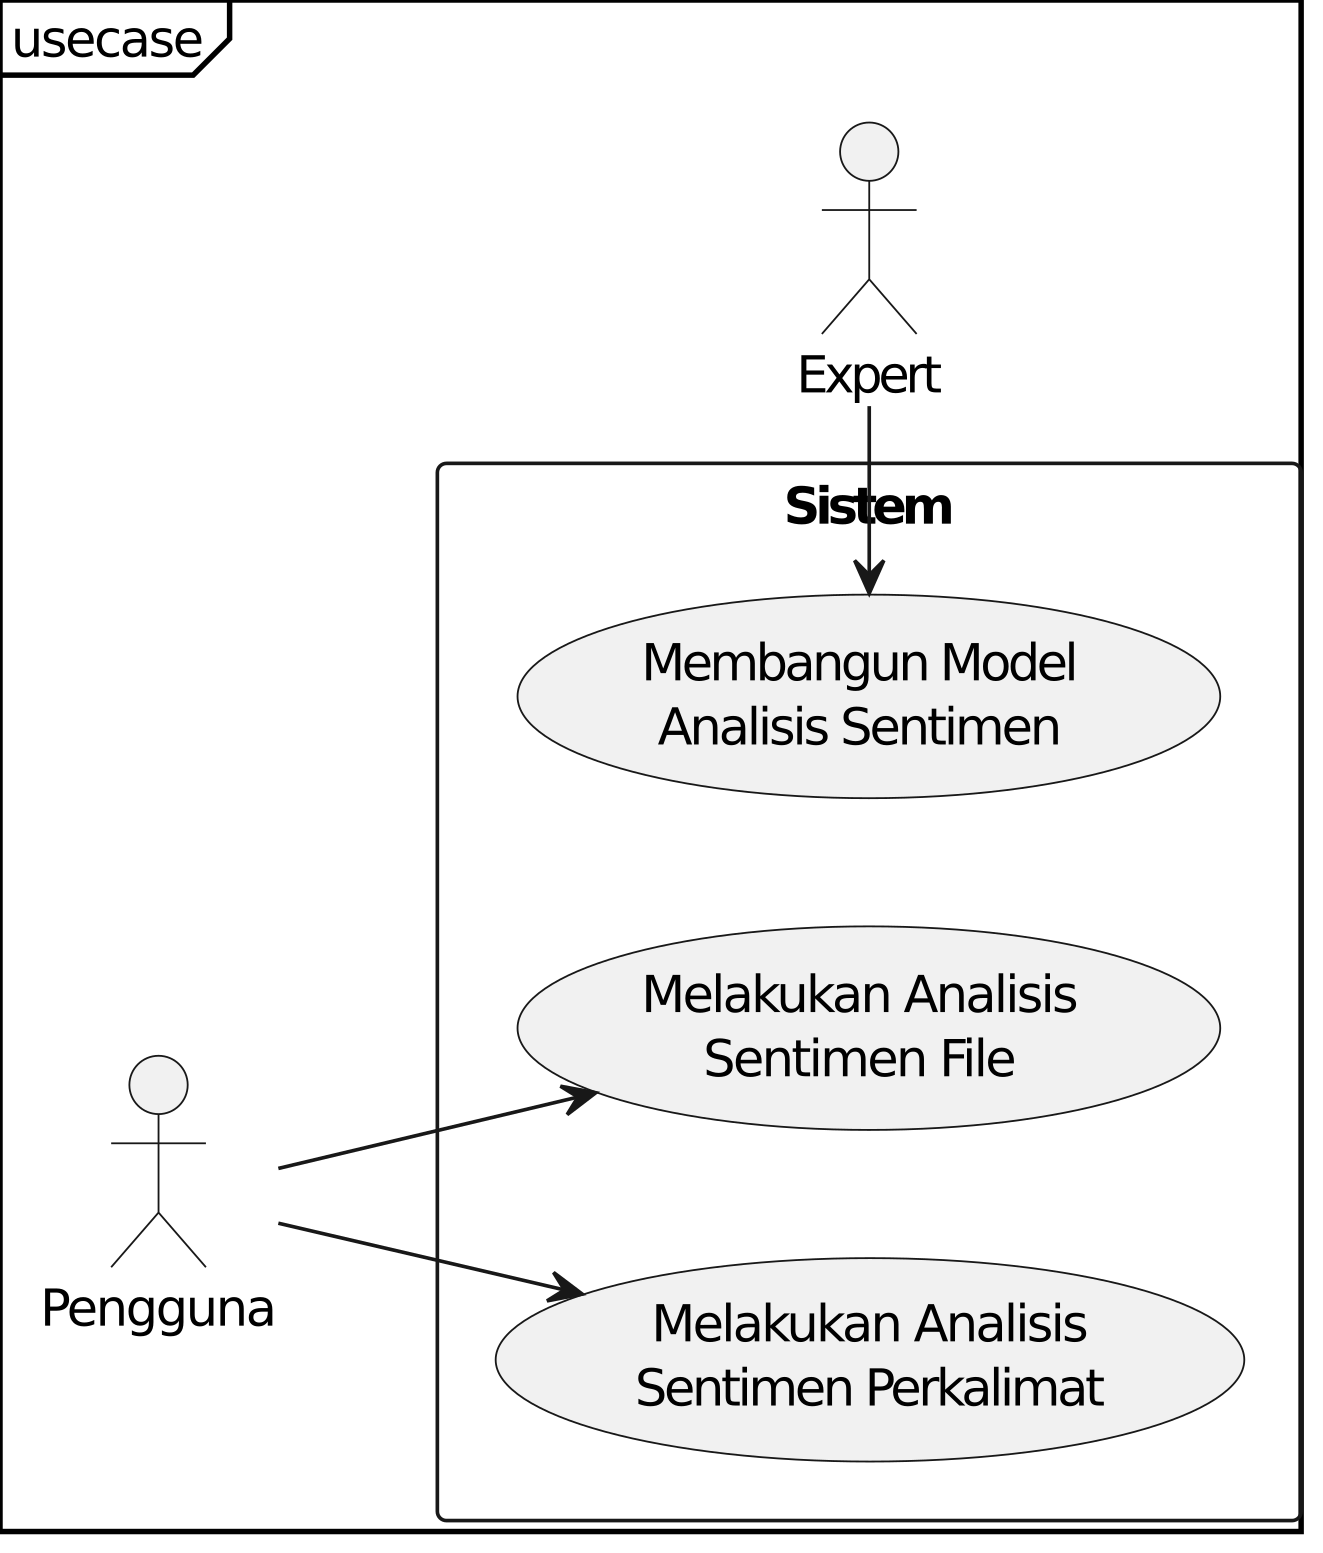
\includegraphics[scale=1]{assets/usecase_diagram.png}
  \caption{Diagram \emph{Use Case}}
  \label{fig:usecase_diagram}
\end{figure}

\subsubsection{Definisi \emph{Use Case}}
Penjelasan lebih detail dari diagram \emph{use case} pada Gambar~\ref{fig:usecase_diagram} diatas dapat dilihat
pada Tabel~\ref{tab:definisi_usecase}.

\begin{table}[H]
  \centering
  \caption{Definisi \emph{Use Case}}
  \label{tab:definisi_usecase}
  \begin{tabularx}{\textwidth}{|l|l|X|}
    \hline
    No & Use Case                        & Keterangan \\ \hline
    1  & \makecell[l]{Melakukan Analisis              \\Sentimen Kalimat} & Salah satu fitur utama dari aplikasi dimana sistem akan menerima masukan berupa kalimat dan menampilkan hasil dari operasi analisis sentimen           \\ \hline
    2  & \makecell[l]{Melakukan Analisis              \\Sentimen File}    & Salah satu fitur utama dari aplikasi dimana sistem akan menerima masukan berupa file berkekstensi~.csv dan menampilkan hasil operasi analisis sentimen \\ \hline
    3  & \makecell[l]{Membangun Model                 \\Analisis Sentimen}    & Dalam usecase ini dilakukan pelatihan model CNN untuk melakukan analisis sentimen dan pengukuran kinerja dari model dengan menggunakan data uji\\ \hline
  \end{tabularx}
\end{table}

\subsubsection{Definisi Aktor}
Aktor merupakan seseorang yang berinteraksi dengan \emph{use case} melalui perangkat lunak yang dikembangkan.
Penjelasan tentang aktor dapat dilihat pada Tabel~\ref{tab:aktor_definisi}.

\begin{table}[H]
  \centering
  \caption{Definisi Aktor}
  \label{tab:aktor_definisi}
  \begin{tabularx}{\columnwidth}{|l|l|X|}
    \hline
    No & Aktor    & Definisi                                                                                                          \\ \hline
    1  & Pengguna & Pengguna adalah seseorang yang ingin menggunakan semua fitur yang terdapat pada perangkat lunak yang dikembangkan \\ \hline
    2  & Expert   & Expert adalah seseorang yang membangun dan mengukur kinerja dari model CNN untuk melakukan analisis sentimen      \\ \hline
  \end{tabularx}
\end{table}

\subsubsection{Skenario \emph{Use Case}}
Skenario \emph{use case} adalah alur dari proses \emph{use case} dari sisi aktor dan sistem.
Setiap \emph{use case} yang ada pada diagram memiliki skenario. Penjelasan tentang skenario untuk setiap
\emph{use case} dapat dilihat pada Tabel~\ref{tab:scenario_usecase_kalimat},~\ref{tab:scenario_usecase_file},~\ref{tab:scenario_usecase_train}.

\begin{longtable}[c]{|ll|}
  \caption{Skenario Usecase Analisis Sentimen Kalimat}
  \label{tab:scenario_usecase_kalimat}                                                                                                                                                                                                                         \\
  \hline
  \multicolumn{2}{|c|}{\textbf{Identifikasi}}                                                                                                                                                                                                                  \\ \hline
  \endhead
  %
  \multicolumn{1}{|l|}{\textbf{Nomor}}                                                                            & UC-01                                                                                                                                      \\ \hline
  \multicolumn{1}{|l|}{\textbf{Nama}}                                                                             & Melakukan analisis sentimen perkalimat                                                                                                     \\ \hline
  \multicolumn{1}{|l|}{\textbf{Aktor}}                                                                            & Pengguna                                                                                                                                   \\ \hline
  \multicolumn{1}{|l|}{\textbf{Tujuan}}                                                                           & Menampilkan hasil dari analisis sentimen                                                                                                   \\ \hline
  \multicolumn{1}{|l|}{\textbf{Deksripsi}}                                                                        &
  \begin{tabular}[c]{@{}l@{}}Dalam usecase ini dilakukan analisis sentimen\\ pada kalimat yang dimasukkan ke text box oleh\\ pengguna  sebagai masukan. Kalimat akan\\ dilakukan klasifikasi menggunakan model yang \\ telah dilatih oleh expert.\end{tabular} \\ \hline
  \multicolumn{1}{|l|}{\textbf{Kondisi Awal}}                                                                     &
  \begin{tabular}[c]{@{}l@{}}Pengguna memasukan data ke text box yang \\ ada di aplikasi android\end{tabular}                                                                                                                                                  \\ \hline
  \multicolumn{2}{|c|}{\textbf{Skenario Normal}}                                                                                                                                                                                                               \\ \hline
  \multicolumn{1}{|l|}{\textbf{Aktor}}                                                                            & \textbf{Sistem}                                                                                                                            \\ \hline
  \multicolumn{1}{|l|}{\begin{tabular}[c]{@{}l@{}}1. Memilih Tab \\ Analisis Sentimen \\ Perkalimat\end{tabular}} &
  \begin{tabular}[c]{@{}l@{}}2. Menampilkan Analisis \\ Sentimen Perkalimat\end{tabular}                                                                                                                                                                       \\ \hline
  \multicolumn{1}{|l|}{}                                                                                          & \begin{tabular}[c]{@{}l@{}}3. Menerima Masukan\\ Berupa Kalimat\end{tabular}                                                               \\ \hline
  \multicolumn{1}{|l|}{}                                                                                          & \begin{tabular}[c]{@{}l@{}}4. Mengklasifikasi Sentimen\\ Positif Atau Negatif\end{tabular}                                                 \\ \hline
  \multicolumn{1}{|l|}{}                                                                                          & \begin{tabular}[c]{@{}l@{}}5. Menampilkan\\ Hasil Klasifikasi\end{tabular}                                                                 \\ \hline
  \multicolumn{1}{|l|}{\textbf{Kondisi Akhir}}                                                                    & \begin{tabular}[c]{@{}l@{}}Sistem menampilkan\\ hasil analisis sentimen\end{tabular}                                                       \\ \hline
\end{longtable}

\begin{longtable}[c]{|ll|}
  \caption{Skenario Usecase Analisis Sentimen File}
  \label{tab:scenario_usecase_file}                                                                                                                                                                                                                                                                                                             \\
  \hline
  \multicolumn{2}{|c|}{\textbf{Identifikasi}}                                                                                                                                                                                                                                                                                                   \\ \hline
  \endhead
  %
  \multicolumn{1}{|l|}{\textbf{Nomor}}                                                                  &
  UC-02                                                                                                                                                                                                                                                                                                                                         \\ \hline
  \multicolumn{1}{|l|}{\textbf{Nama}}                                                                   &
  Melakukan analisis sentimen file                                                                                                                                                                                                                                                                                                              \\ \hline
  \multicolumn{1}{|l|}{\textbf{Aktor}}                                                                  &
  Pengguna                                                                                                                                                                                                                                                                                                                                      \\ \hline
  \multicolumn{1}{|l|}{\textbf{Tujuan}}                                                                 &
  Menampilkan hasil dari analisis sentimen                                                                                                                                                                                                                                                                                                      \\ \hline
  \multicolumn{1}{|l|}{\textbf{Deksripsi}}                                                              &
  \begin{tabular}[c]{@{}l@{}}Dalam usecase ini dilakukan analisis sentimen \\ pada file berekstensi .csv yang berisi sentimen\\ sentimen dengan tiga kolom yang terdiri dari indeks,\\ sentimen, dan label oleh pengguna sebagai masukan.\\ Kalimat akan dilakukan klasifikasi menggunakan\\ model yang telah dilatih oleh expert.\end{tabular} \\ \hline
  \multicolumn{1}{|l|}{\textbf{Kondisi   Awal}}                                                         &
  \begin{tabular}[c]{@{}l@{}}Pengguna memasukan data ke text box yang ada \\ di aplikasi android\end{tabular}                                                                                                                                                                                                                                   \\ \hline
  \multicolumn{2}{|l|}{\textbf{Skenario Normal}}                                                                                                                                                                                                                                                                                                \\ \hline
  \multicolumn{1}{|l|}{\textbf{Aktor}}                                                                  &
  \textbf{Sistem}                                                                                                                                                                                                                                                                                                                               \\ \hline
  \multicolumn{1}{|l|}{\begin{tabular}[c]{@{}l@{}}1. Memilih tab analisis\\ sentimen file\end{tabular}} &
  2. Menampilkan analisis sentimen file                                                                                                                                                                                                                                                                                                         \\ \hline
  \multicolumn{1}{|l|}{}                                                                                &
  \begin{tabular}[c]{@{}l@{}}3. Menerima masukan berupa file berkestensi .csv\\ yang memiliki tiga kolom yang terdiri dari indeks,\\ sentimen, dan label\end{tabular}                                                                                                                                                                           \\ \hline
  \multicolumn{1}{|l|}{}                                                                                &
  4. Mengklasifikasi sentimen positif atau negatif                                                                                                                                                                                                                                                                                              \\ \hline
  \multicolumn{1}{|l|}{}                                                                                &
  5. Menampilkan hasil klasifikasi                                                                                                                                                                                                                                                                                                              \\ \hline
  \multicolumn{1}{|l|}{\textbf{Kondisi   Akhir}}                                                        &
  Sistem menampilkan hasil analisis sentimen                                                                                                                                                                                                                                                                                                    \\ \hline
\end{longtable}

\begin{longtable}[c]{|ll|}
  \caption{Skenario Usecase Analisis Sentimen Pelatihan}
  \label{tab:scenario_usecase_train}                                                                                                                                                                                                                                                                                                                                                 \\
  \hline
  \multicolumn{2}{|c|}{\textbf{Identifikasi}}                                                                                                                                                                                                                                                                                                                                        \\ \hline
  \endhead
  %
  \multicolumn{1}{|l|}{\textbf{Nomor}}                                                        &
  UC-03                                                                                                                                                                                                                                                                                                                                                                              \\ \hline
  \multicolumn{1}{|l|}{\textbf{Nama}}                                                         &
  Membangun model CNN untuk melakukan analisis sentimen                                                                                                                                                                                                                                                                                                                              \\ \hline
  \multicolumn{1}{|l|}{\textbf{Aktor}}                                                        &
  Expert                                                                                                                                                                                                                                                                                                                                                                             \\ \hline
  \multicolumn{1}{|l|}{\textbf{Tujuan}}                                                       &
  \begin{tabular}[c]{@{}l@{}}Menampilkan kinerja model CNN berupa akurasi, presisi, \\ recall  dan f1-score\end{tabular}                                                                                                                                                                                                                                                             \\ \hline
  \multicolumn{1}{|l|}{\textbf{Deksripsi}}                                                    &
  \begin{tabular}[c]{@{}l@{}}Dalam usecase ini dilakukan pelatihan model CNN untuk \\ melakukan analisis sentimen dengan menggunakan data\\ latih  dengan jumlah 3600 yang terdiri dari 1800 label positif\\ dan 1800 label negatif dan di validasi dengan  menggunakan\\ data validasi yang berjumlah 1200 yang terdiri dari 600 label\\ positif dan 600 label negatif\end{tabular} \\ \hline
  \multicolumn{1}{|l|}{\textbf{Kondisi Awal}}                                                 &
  Google Colab dalam kondisi belum tereksekusi                                                                                                                                                                                                                                                                                                                                       \\ \hline
  \multicolumn{2}{|c|}{\textbf{Skenario Normal}}                                                                                                                                                                                                                                                                                                                                     \\ \hline
  \multicolumn{1}{|l|}{\textbf{Aktor}}                                                        &
  \textbf{Sistem}                                                                                                                                                                                                                                                                                                                                                                    \\ \hline
  \multicolumn{1}{|l|}{\begin{tabular}[c]{@{}l@{}}1. Menekan\\ Tombol\\ Run All\end{tabular}} &
  2. Melakukan praproses pada teks                                                                                                                                                                                                                                                                                                                                                   \\ \hline
  \multicolumn{1}{|l|}{}                                                                      &
  3. Mengubah kata menjadi word embedding                                                                                                                                                                                                                                                                                                                                            \\ \hline
  \multicolumn{1}{|l|}{}                                                                      &
  4. Melakukan pelatihan model                                                                                                                                                                                                                                                                                                                                                       \\ \hline
  \multicolumn{1}{|l|}{}                                                                      &
  5. Menyimpan model yang telah dilatih                                                                                                                                                                                                                                                                                                                                              \\ \hline
  \multicolumn{1}{|l|}{}                                                                      &
  6. Menampilkan laporan hasil klasifikasi                                                                                                                                                                                                                                                                                                                                           \\ \hline
  \multicolumn{1}{|l|}{\textbf{Kondisi Akhir}}                                                &
  Sistem menampilkan hasil analisis sentimen                                                                                                                                                                                                                                                                                                                                         \\ \hline
\end{longtable}

\section{Fase Elaborasi}
Fase kedua atau fase elaborasi dalam fase ini terdapat aktivitas yang dilakukan yaitu pemodelan bisinis, perancangan antarmuka
pengguna atau \emph{user interface}, dan pembuatan \emph{sequence diagram}.

\subsection{Pemodelan Bisnis}
Pemodelan bisnis pada fase ini adalah melakukan perancangan perangkat lunak berdasarkan fase insepsi yang telah dilakukan
pada \autoref{fase_insepsi} sebelumnya. Perancangan yang dilakukan yaitu antarmuka () dan pembuatan
\emph{sequence diagram}.

\subsection{Perancangan Antarmuka (\emph{Interface})}
Terdapat dua halaman rancangan yang dibuat berdasarkan pada Fase Insepsi sebelumnya. Desain antarmuka
dapat dilihat pada Gambar~\ref{fig:rancangan_interface_kalimat} dan Gambar~\ref{fig:rancangan_interface_file}

\begin{figure}[H]
  \centering
  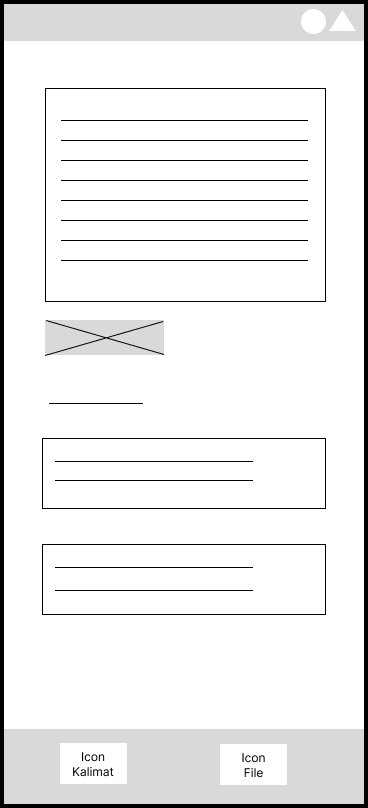
\includegraphics[width=4cm, height=8cm]{assets/rancangan_interface_kalimat.png}
  \caption{Rancangan Antarmuka Kalimat}
  \label{fig:rancangan_interface_kalimat}
\end{figure}

\begin{figure}[H]
  \centering
  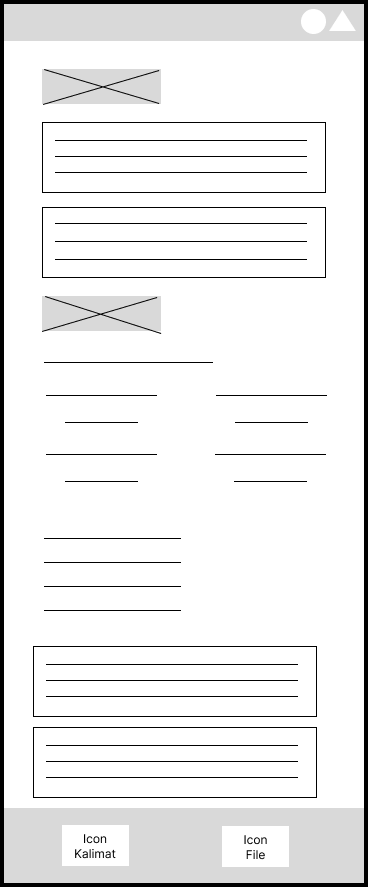
\includegraphics[width=4cm, height=8cm]{assets/rancangan_interface_file.png}
  \caption{Rancangan Antarmuka File}
  \label{fig:rancangan_interface_file}
\end{figure}

\subsection{Diagram Aktivitas}
Diagram aktivitas digunakan untuk mengilustrasikan alur kegiatan atau aktivitas dari sebuah
perangkat lunak yang dikembangkan sesuai pada pemodelan proses bisnis. Diagram aktivitas dapat dilihat
pada Gambar~\ref{fig:activity_diagram_kalimat} dan pada Gambar~\ref{fig:activity_diagram_file}.

\begin{figure}[H]
  \centering
  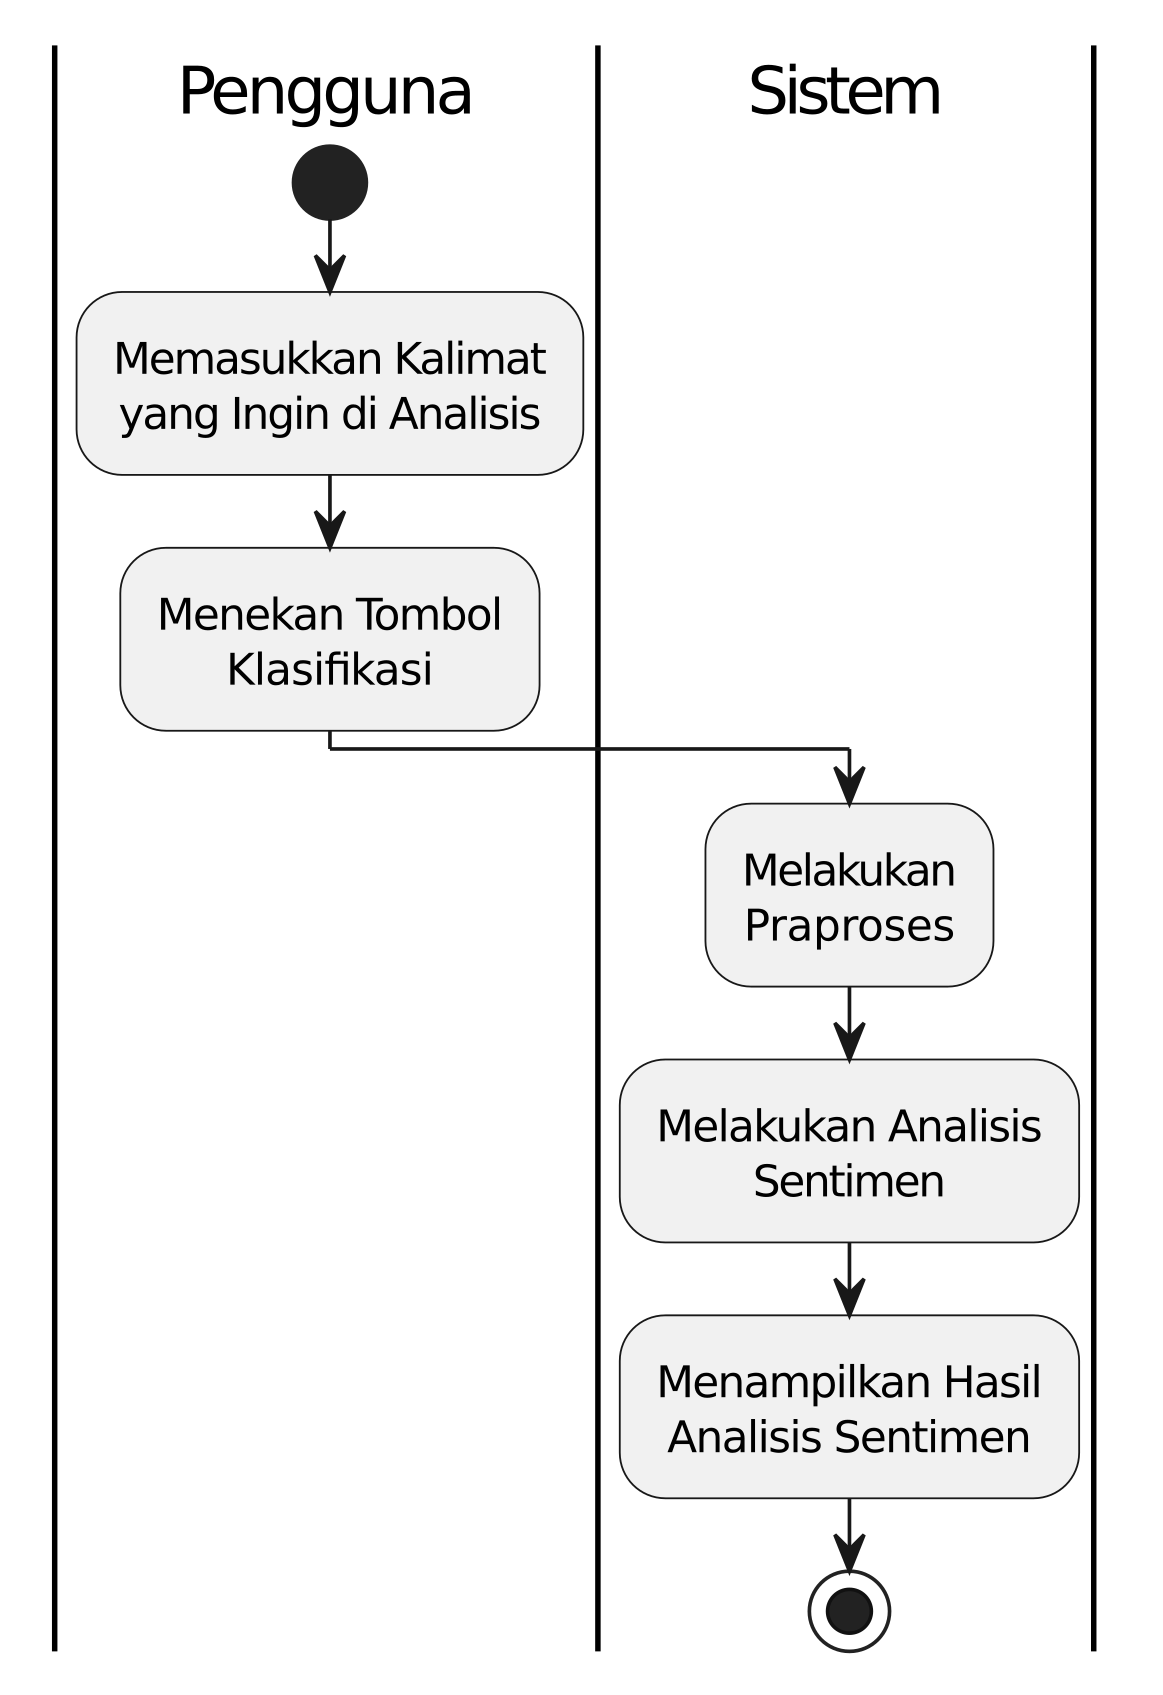
\includegraphics[scale=0.7]{assets/activity_diagram_kalimat.png}
  \caption{Diagram Aktivitas Kalimat}
  \label{fig:activity_diagram_kalimat}
\end{figure}

\begin{figure}[H]
  \centering
  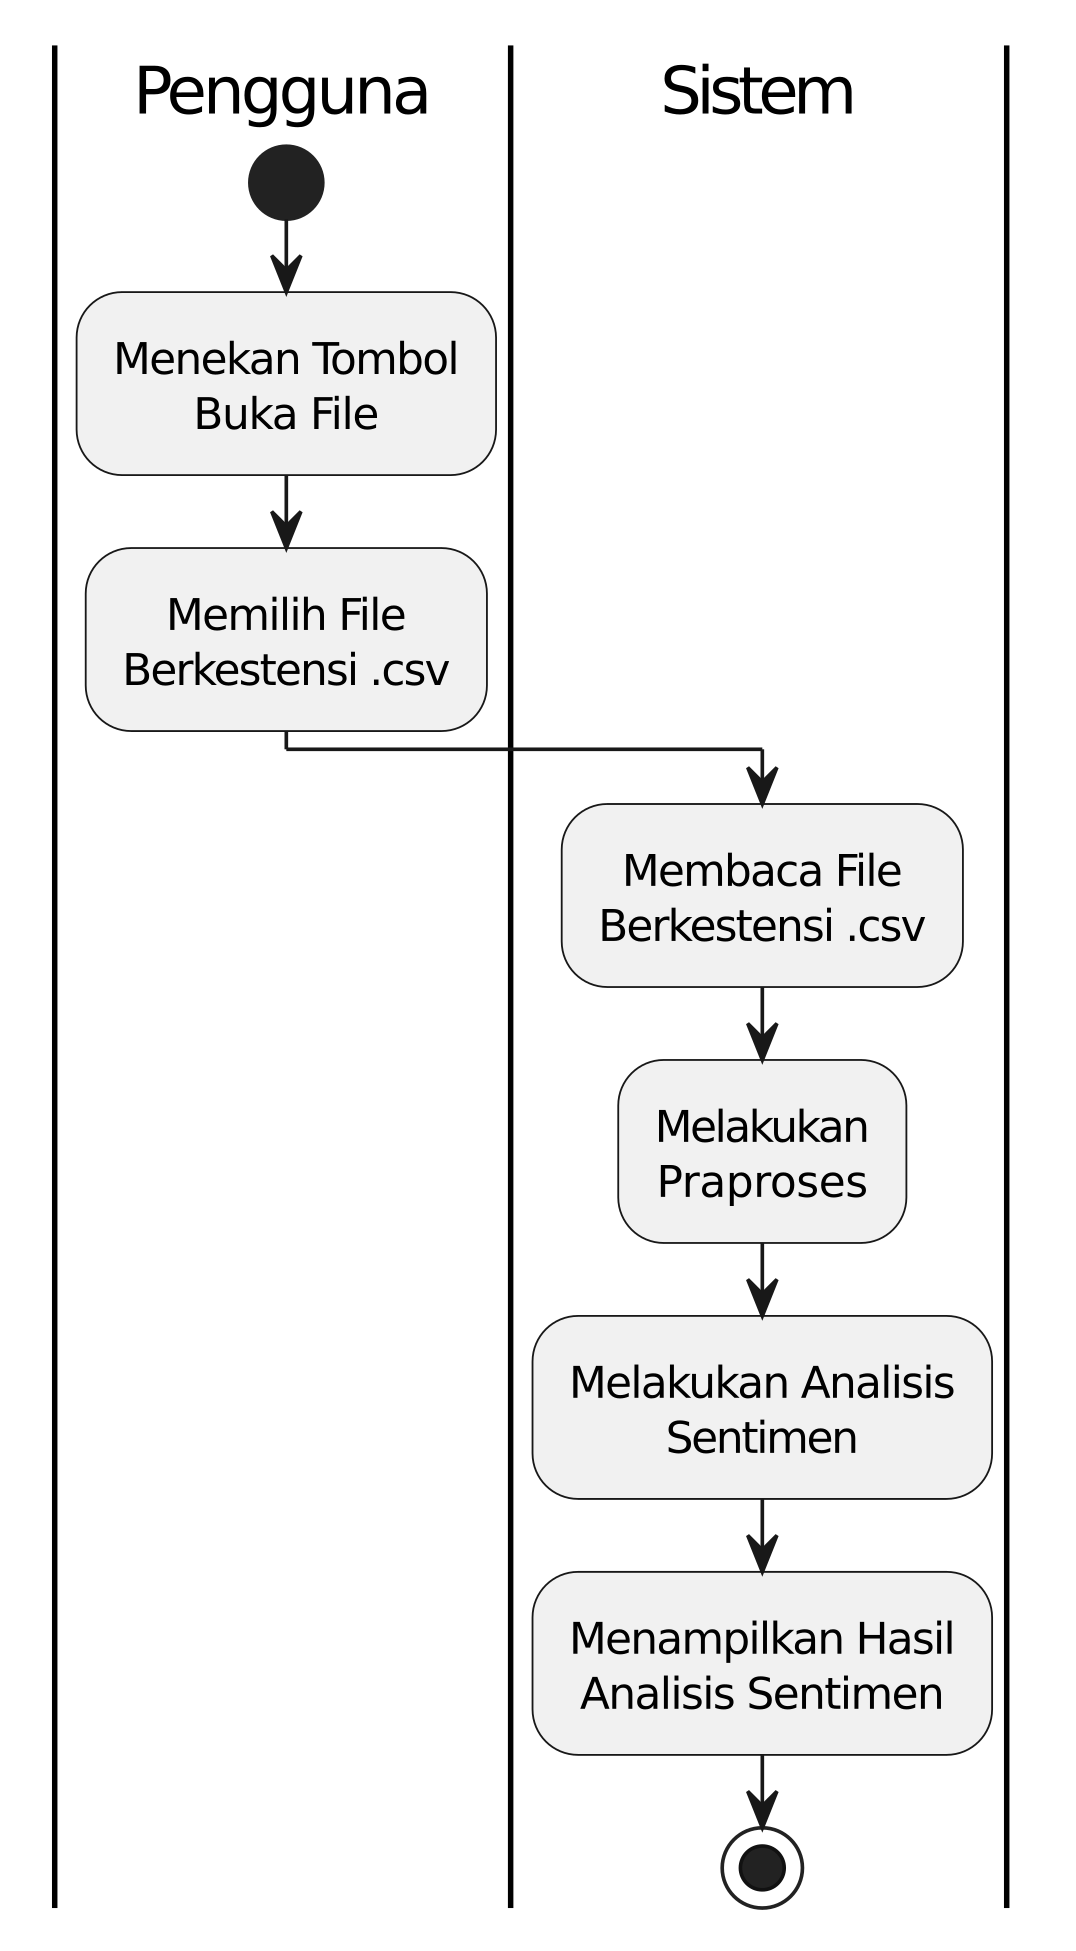
\includegraphics[scale=0.7]{assets/activity_diagram_file.png}
  \caption{Diagram Aktivitas File}
  \label{fig:activity_diagram_file}
\end{figure}

\begin{figure}[H]
  \centering
  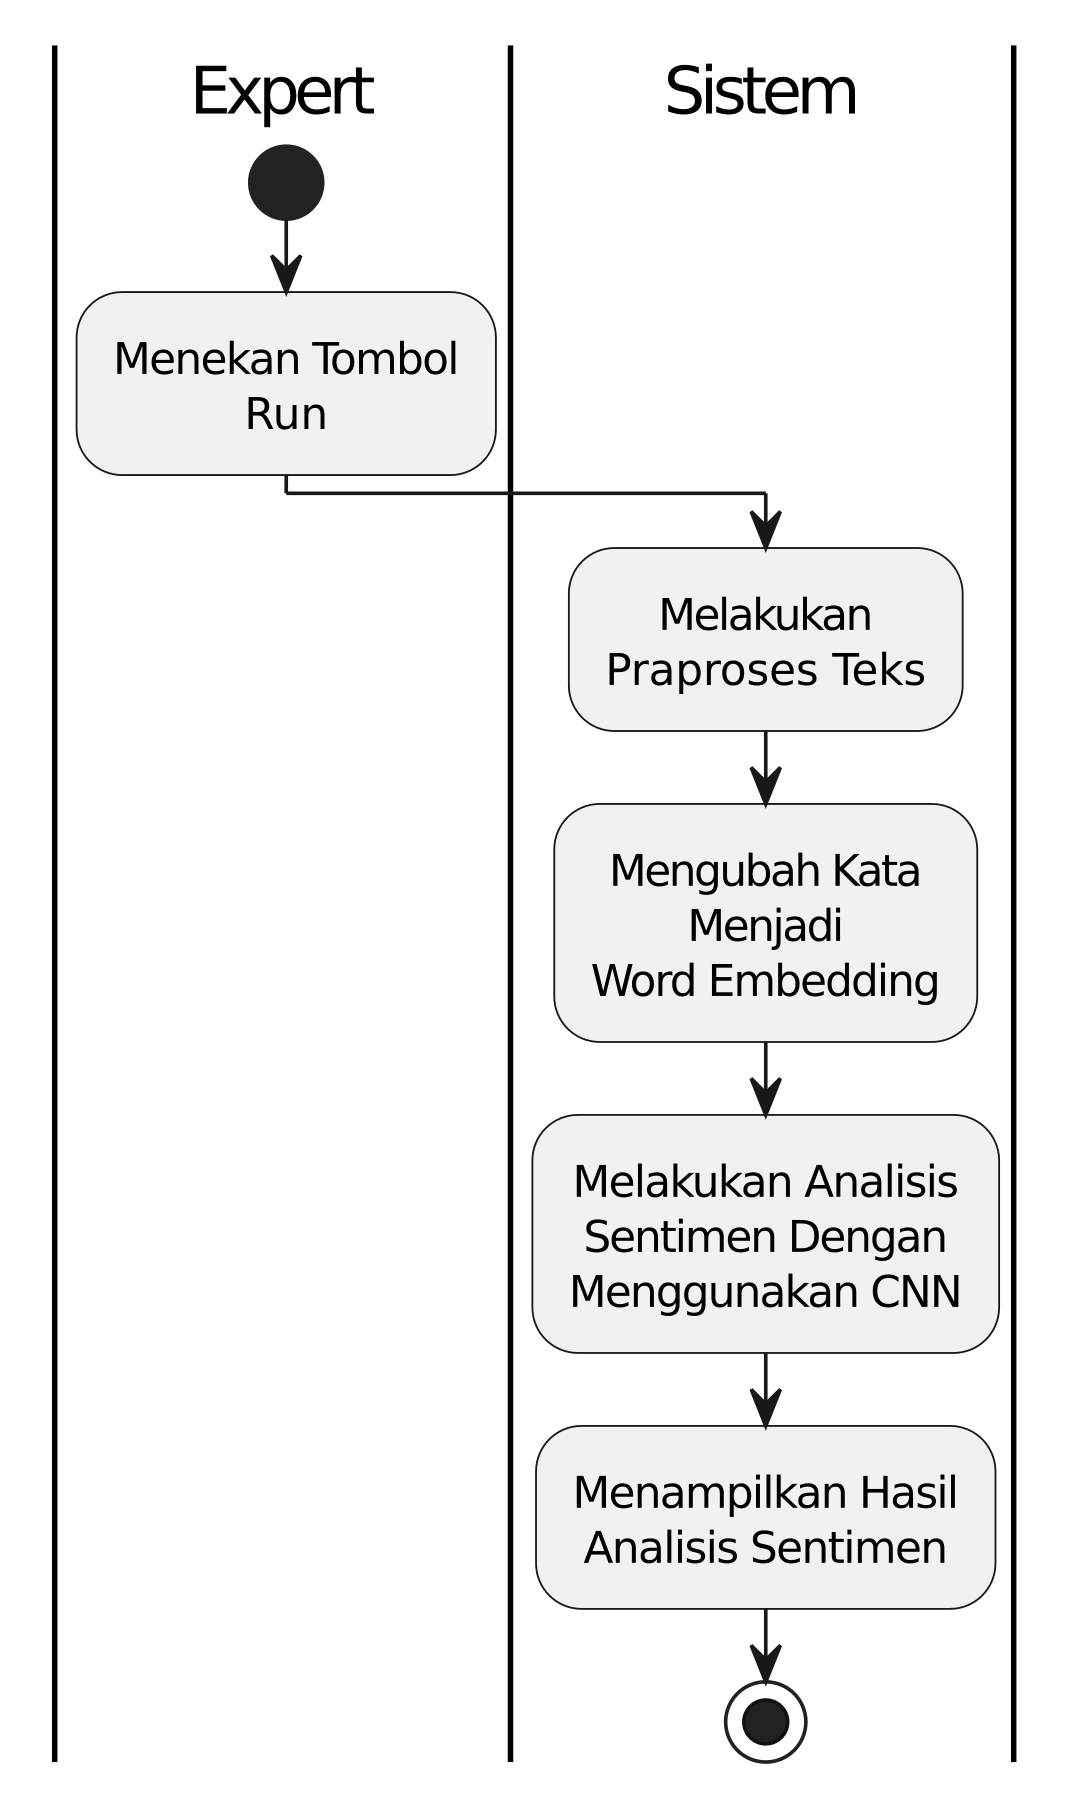
\includegraphics[scale=0.7]{assets/activity_diagram_test.png}
  \caption{Diagram Aktivitas Pengujian}
  \label{fig:activity_diagram_kalimat}
\end{figure}

\subsection{\emph{Sequence Diagram}}
Pada Sub Bagian \emph{Sequence Diagram} ini akan dijelaskan alur interaksi pada setiap objek didalam
perangkat lunak berdasarkan \emph{Use Case} yang telah dirancang. \emph{Sequence diagram} dapat dilihat
pada Gambar~\ref{fig:sequence_diagram_kalimat} dan Gambar~\ref{fig:sequence_diagram_file}.

\begin{figure}[H]
  \centering
  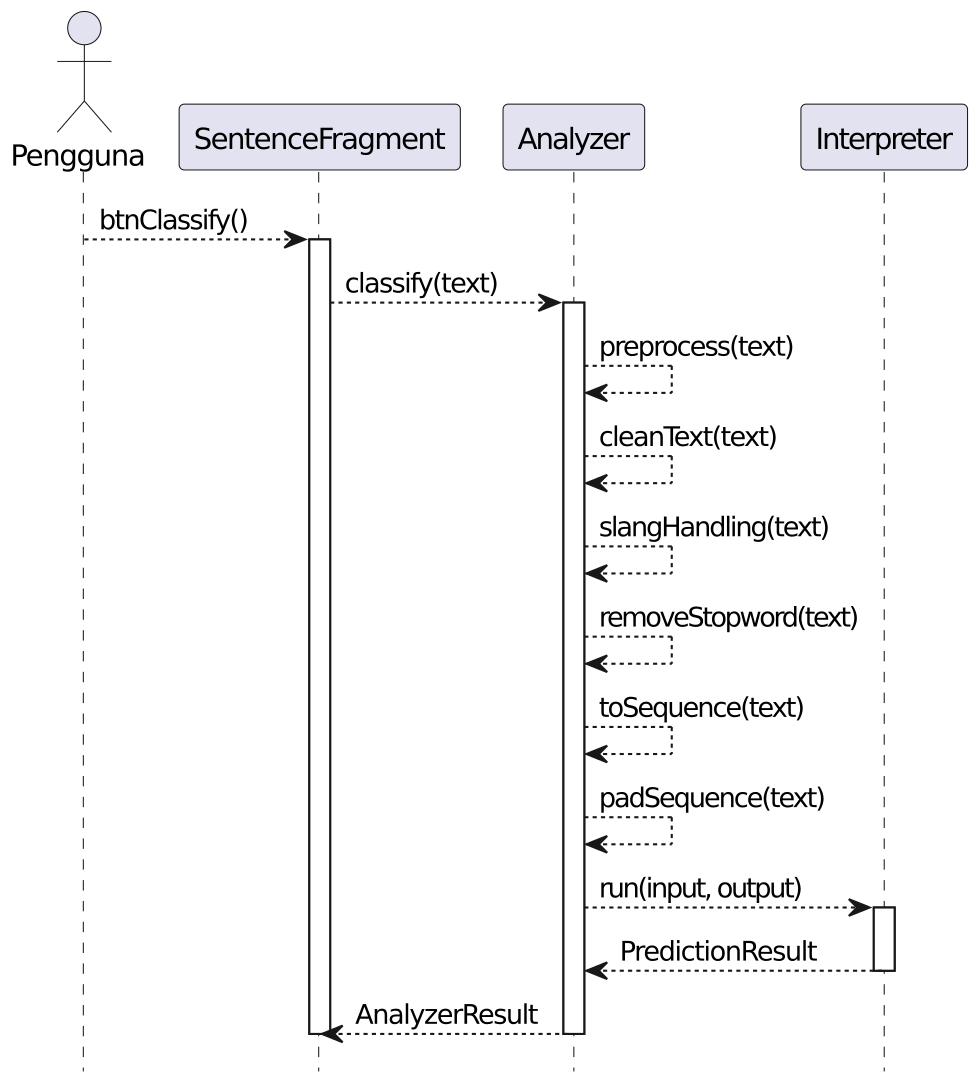
\includegraphics[width=\textwidth]{assets/sequence_diagram_kalimat.png}
  \caption{Sequence Diagram Kalimat}
  \label{fig:sequence_diagram_kalimat}
\end{figure}

\begin{figure}[H]
  \centering
  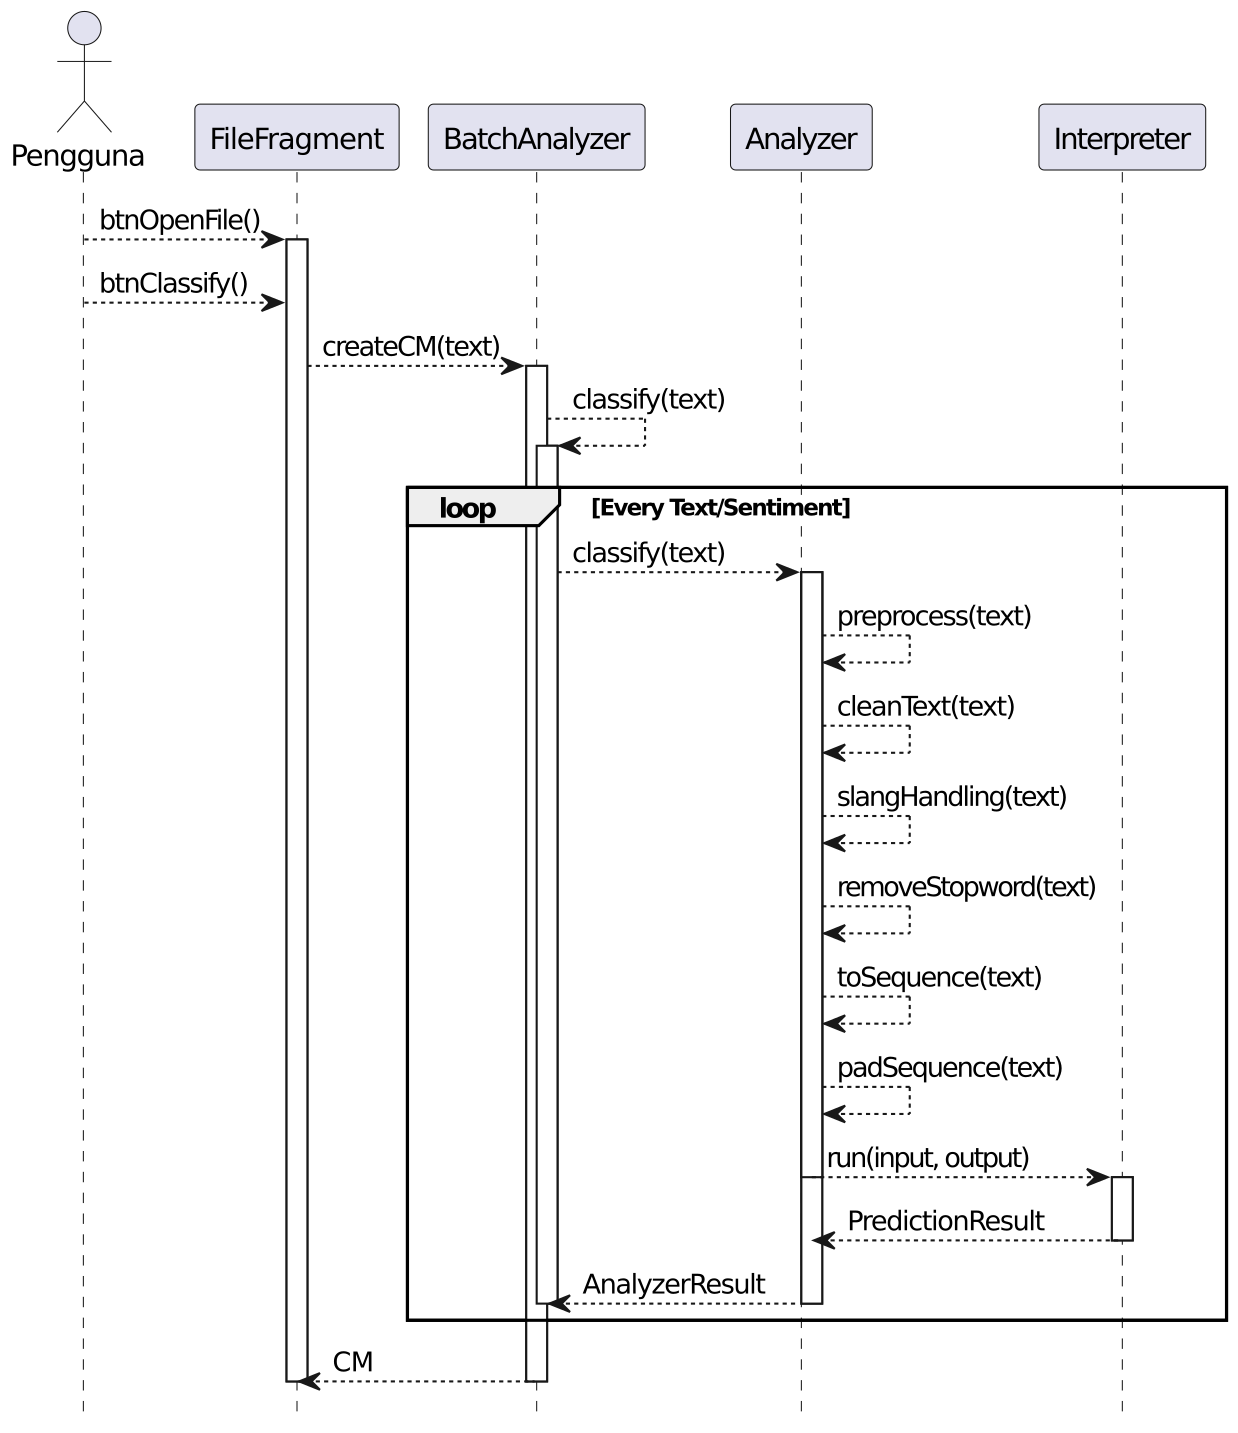
\includegraphics[width=\textwidth]{assets/sequence_diagram_file.png}
  \caption{Sequence Diagram File}
  \label{fig:sequence_diagram_file}
\end{figure}

\begin{figure}[H]
  \centering
  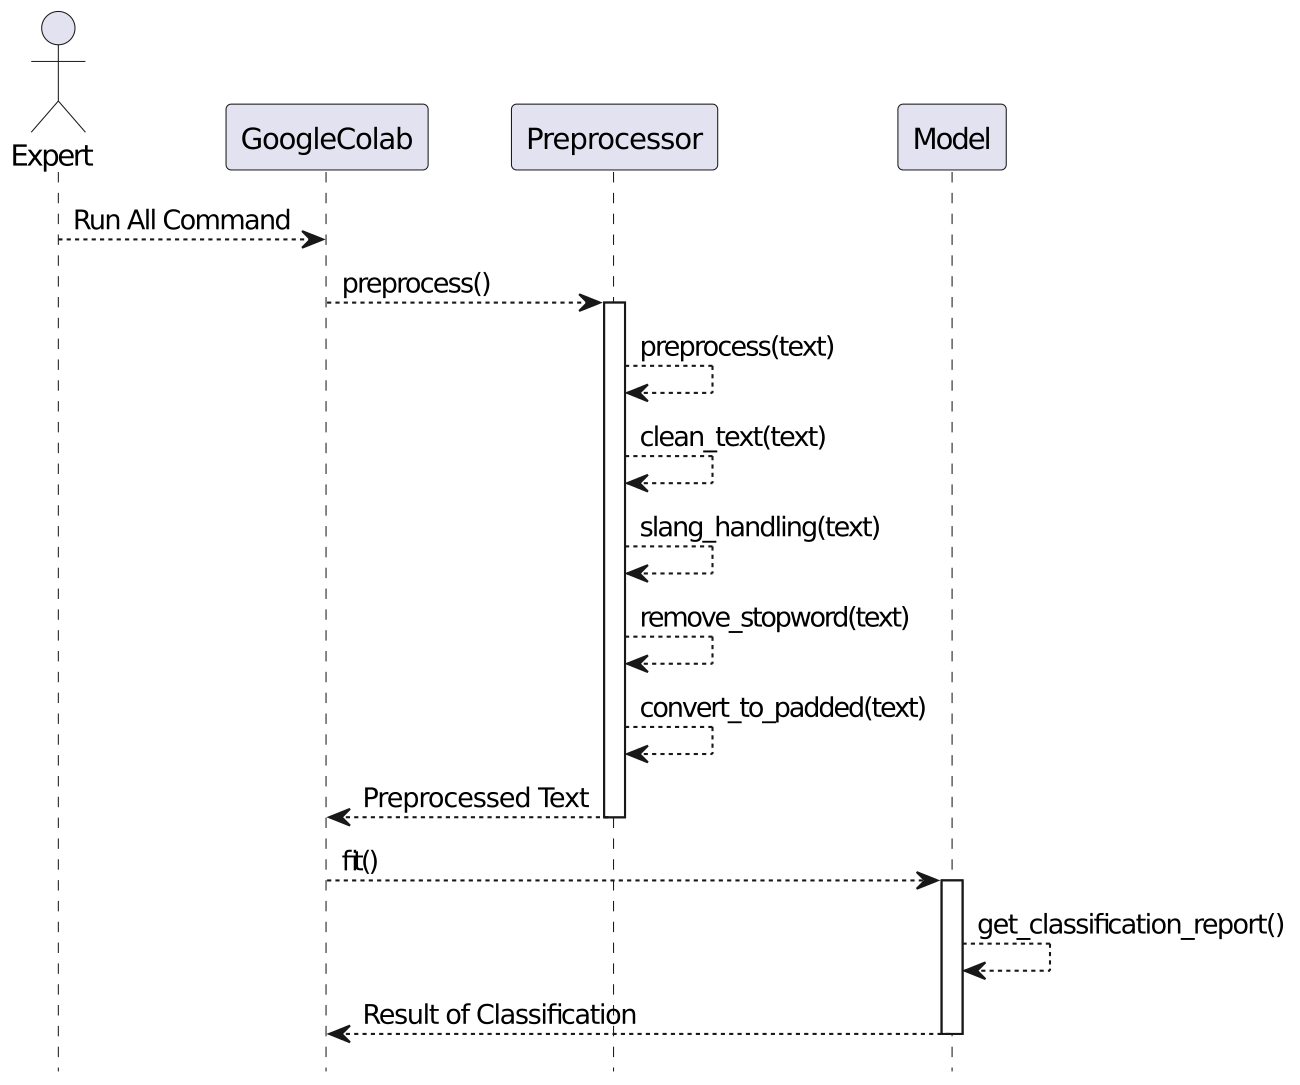
\includegraphics[width=\textwidth]{assets/sequence_diagram_test.png}
  \caption{Sequence Diagram Pengujian}
  \label{fig:sequence_diagram_test}
\end{figure}


\section{Fase Konstruksi}
Fase ketiga atau Fase Konstruksi dalam fase ini terdapat langkah-langkah yang harus dilakukan yaitu
pemodelan diagram kelas dan melakukan implementasi dari rancangan antarmuka (\emph{interface})
program dan diagram kelas.

\subsection{Diagram Kelas}
Diagram kelas atau umumnya dikenal sebagai diagram UML yang menjelaskan deksripsi, relasi, atribut, dan metode yang
ada dikelas dari perangkat lunak yang dikembangkan. Diagram kelas dapat dilihat pada
Gambar~\ref{fig:class_diagram_kalimat} dan pada Gambar~\ref{fig:class_diagram_file}.

\begin{figure}[H]
  \centering
  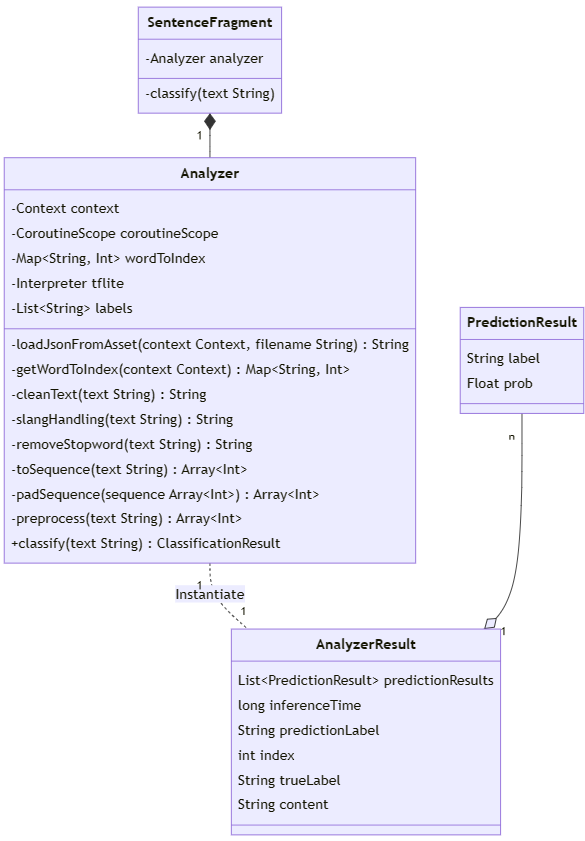
\includegraphics[scale=0.67]{assets/class_diagram_kalimat.png}
  \caption{Diagram Kelas Kalimat}
  \label{fig:class_diagram_kalimat}
\end{figure}

\begin{figure}[H]
  \centering
  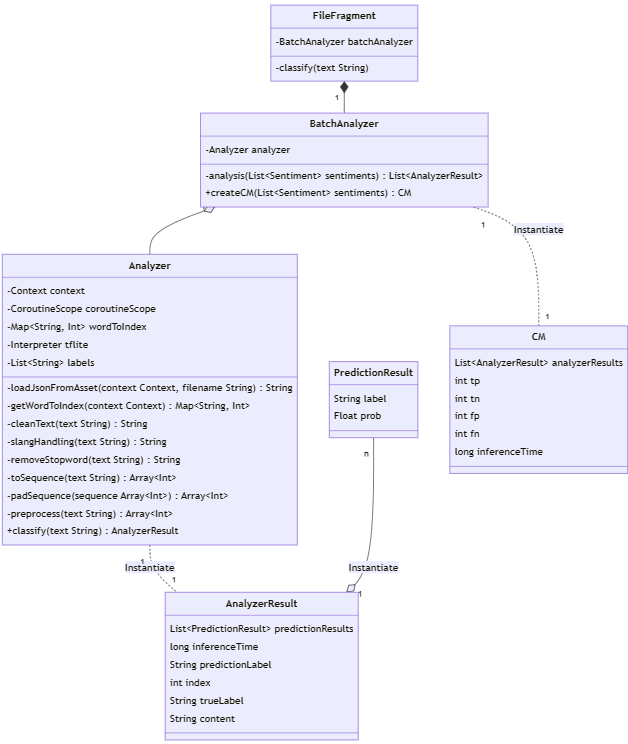
\includegraphics[width=\textwidth]{assets/class_diagram_file.png}
  \caption{Diagram Kelas File}
  \label{fig:class_diagram_file}
\end{figure}

\begin{figure}[H]
  \centering
  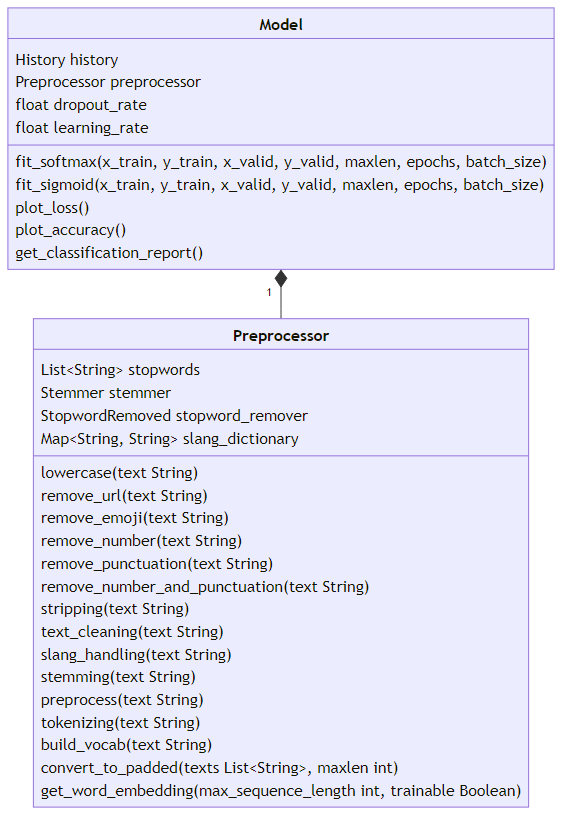
\includegraphics[scale=0.4]{assets/class_diagram_test.png}
  \caption{Diagram Kelas Pengujian}
  \label{fig:class_diagram_kalimat}
\end{figure}

\subsection{Implementasi Diagram Kelas}
Kelas yang telah dirancang dalam bentuk diagram kelas pada Gambar~\ref{fig:class_diagram_file} dan pada
Gambar~\ref{fig:class_diagram_kalimat} diimplementasikan pada program dengan
menggunakan bahasa pemrograman \emph{kotlin}. Pada Tabel~\ref{tab:class_implementation} adalah daftar
kelas yang sudah diimplementasikan ke dalam bentuk kode program.

\begin{longtable}[c]{|l|l|l|l|}
  \caption{Implementasi Diagram Kelas}
  \label{tab:class_implementation}                                                                                                                                                                                        \\
  \hline
  No                                                             &
  \multicolumn{1}{c|}{Nama Kelas}                                &
  \multicolumn{1}{c|}{Nama File}                                 &
  \multicolumn{1}{c|}{Keterangan}                                                                                                                                                                                         \\ \hline
  %
  \endhead
  \hline
  \endfoot
  %
  1                                                              &
  \begin{tabular}[c]{@{}l@{}}Sentence\\ Fragment\end{tabular}    &
  \begin{tabular}[c]{@{}l@{}}Sentence\\ Fragment.kt\end{tabular} &
  \begin{tabular}[c]{@{}l@{}}Kelas yang mengatur tampilan dan interaksi \\ dari fitur Analisis Sentimen Perkalimat\end{tabular}                                                                                           \\ \hline
  2                                                              &
  \begin{tabular}[c]{@{}l@{}}File\\ Fragment\end{tabular}        &
  \begin{tabular}[c]{@{}l@{}}File\\ Fragment.kt\end{tabular}     &
  \begin{tabular}[c]{@{}l@{}}Kelas yang mengatur tampilan dan \\ interaksi dari fitur Analisis Sentimen File\end{tabular}                                                                                                 \\ \hline
  3                                                              &
  \begin{tabular}[c]{@{}l@{}}Prediction\\ Result\end{tabular}    &
  \begin{tabular}[c]{@{}l@{}}Prediction\\ Result.kt\end{tabular} &
  \begin{tabular}[c]{@{}l@{}}Kelas yang menampung hasil dari prediksi \\ sentimen berupa label dan probabilitasnya\end{tabular}                                                                                           \\ \hline
  4                                                              &
  \begin{tabular}[c]{@{}l@{}}Analyzer\\ Result\end{tabular}      &
  \begin{tabular}[c]{@{}l@{}}Analyzer\\ Result.kt\end{tabular}   &
  \begin{tabular}[c]{@{}l@{}}Kelas yang menampung hasil dari prediksi \\ sentimen berapa lama proses prediksi untuk\\ satu sentimen, label yang diprediksi,\\ label yang asli,  index, dan kalimat sentimen.\end{tabular} \\ \hline
  5                                                              &
  \begin{tabular}[c]{@{}l@{}}CM\end{tabular}                     &
  \begin{tabular}[c]{@{}l@{}}CM.kt\end{tabular}                  &
  \begin{tabular}[c]{@{}l@{}}Kelas yang menampung hasil dari analisis\\ sentimen, true positive, true negative, false\\ positive,  false negative, dan berapa lama\\ proses analisis sentimen\end{tabular}                \\ \hline
  6                                                              &
  Sentiment                                                      &
  Sentiment.kt                                                   &
  \begin{tabular}[c]{@{}l@{}}Kelas yang menampung data sentimen\\ dari  file~.csv, berupa index, \\ kalimat sentiment,  dan labelnya\end{tabular}                                                                         \\ \hline
  8                                                              &
  \begin{tabular}[c]{@{}l@{}}Analyzer\end{tabular}               &
  \begin{tabular}[c]{@{}l@{}}Analyzer.kt\end{tabular}            &
  \begin{tabular}[c]{@{}l@{}}Kelas yang melakukan praproses dan \\ analisis  sentimen berdasarkan  kalimat\end{tabular}                                                                                                   \\ \hline
  9                                                              &
  \begin{tabular}[c]{@{}l@{}}Batch\\ Analyzer\end{tabular}       &
  \begin{tabular}[c]{@{}l@{}}Batch\\ Analyzer.kt\end{tabular}    &
  \begin{tabular}[c]{@{}l@{}}Kelas yang melakukan analisis sentiment \\ dari file~.csv dan menghasilkan \\ CM\end{tabular}                                                                                                \\ \hline
  10                                                             &
  \begin{tabular}[c]{@{}l@{}}Model\end{tabular}                  &
  \begin{tabular}[c]{@{}l@{}}model.py\end{tabular}               &
  \begin{tabular}[c]{@{}l@{}}Kelas yang melakukan pelatihan \\ dan pengujian analisis sentimen \\ dengan menggunakan CNN\end{tabular}                                                                                     \\ \hline
  11                                                             &
  \begin{tabular}[c]{@{}l@{}}Preprocessor\end{tabular}           &
  \begin{tabular}[c]{@{}l@{}}preprocessor.py\end{tabular}        &
  \begin{tabular}[c]{@{}l@{}}Kelas yang melakukan praproses pada data\end{tabular}                                                                                                                                        \\ \hline
\end{longtable}

\subsection{Implementasi Antarmuka (\emph{Interface}) Program}
\begin{figure}[H]
  \centering
  \fbox{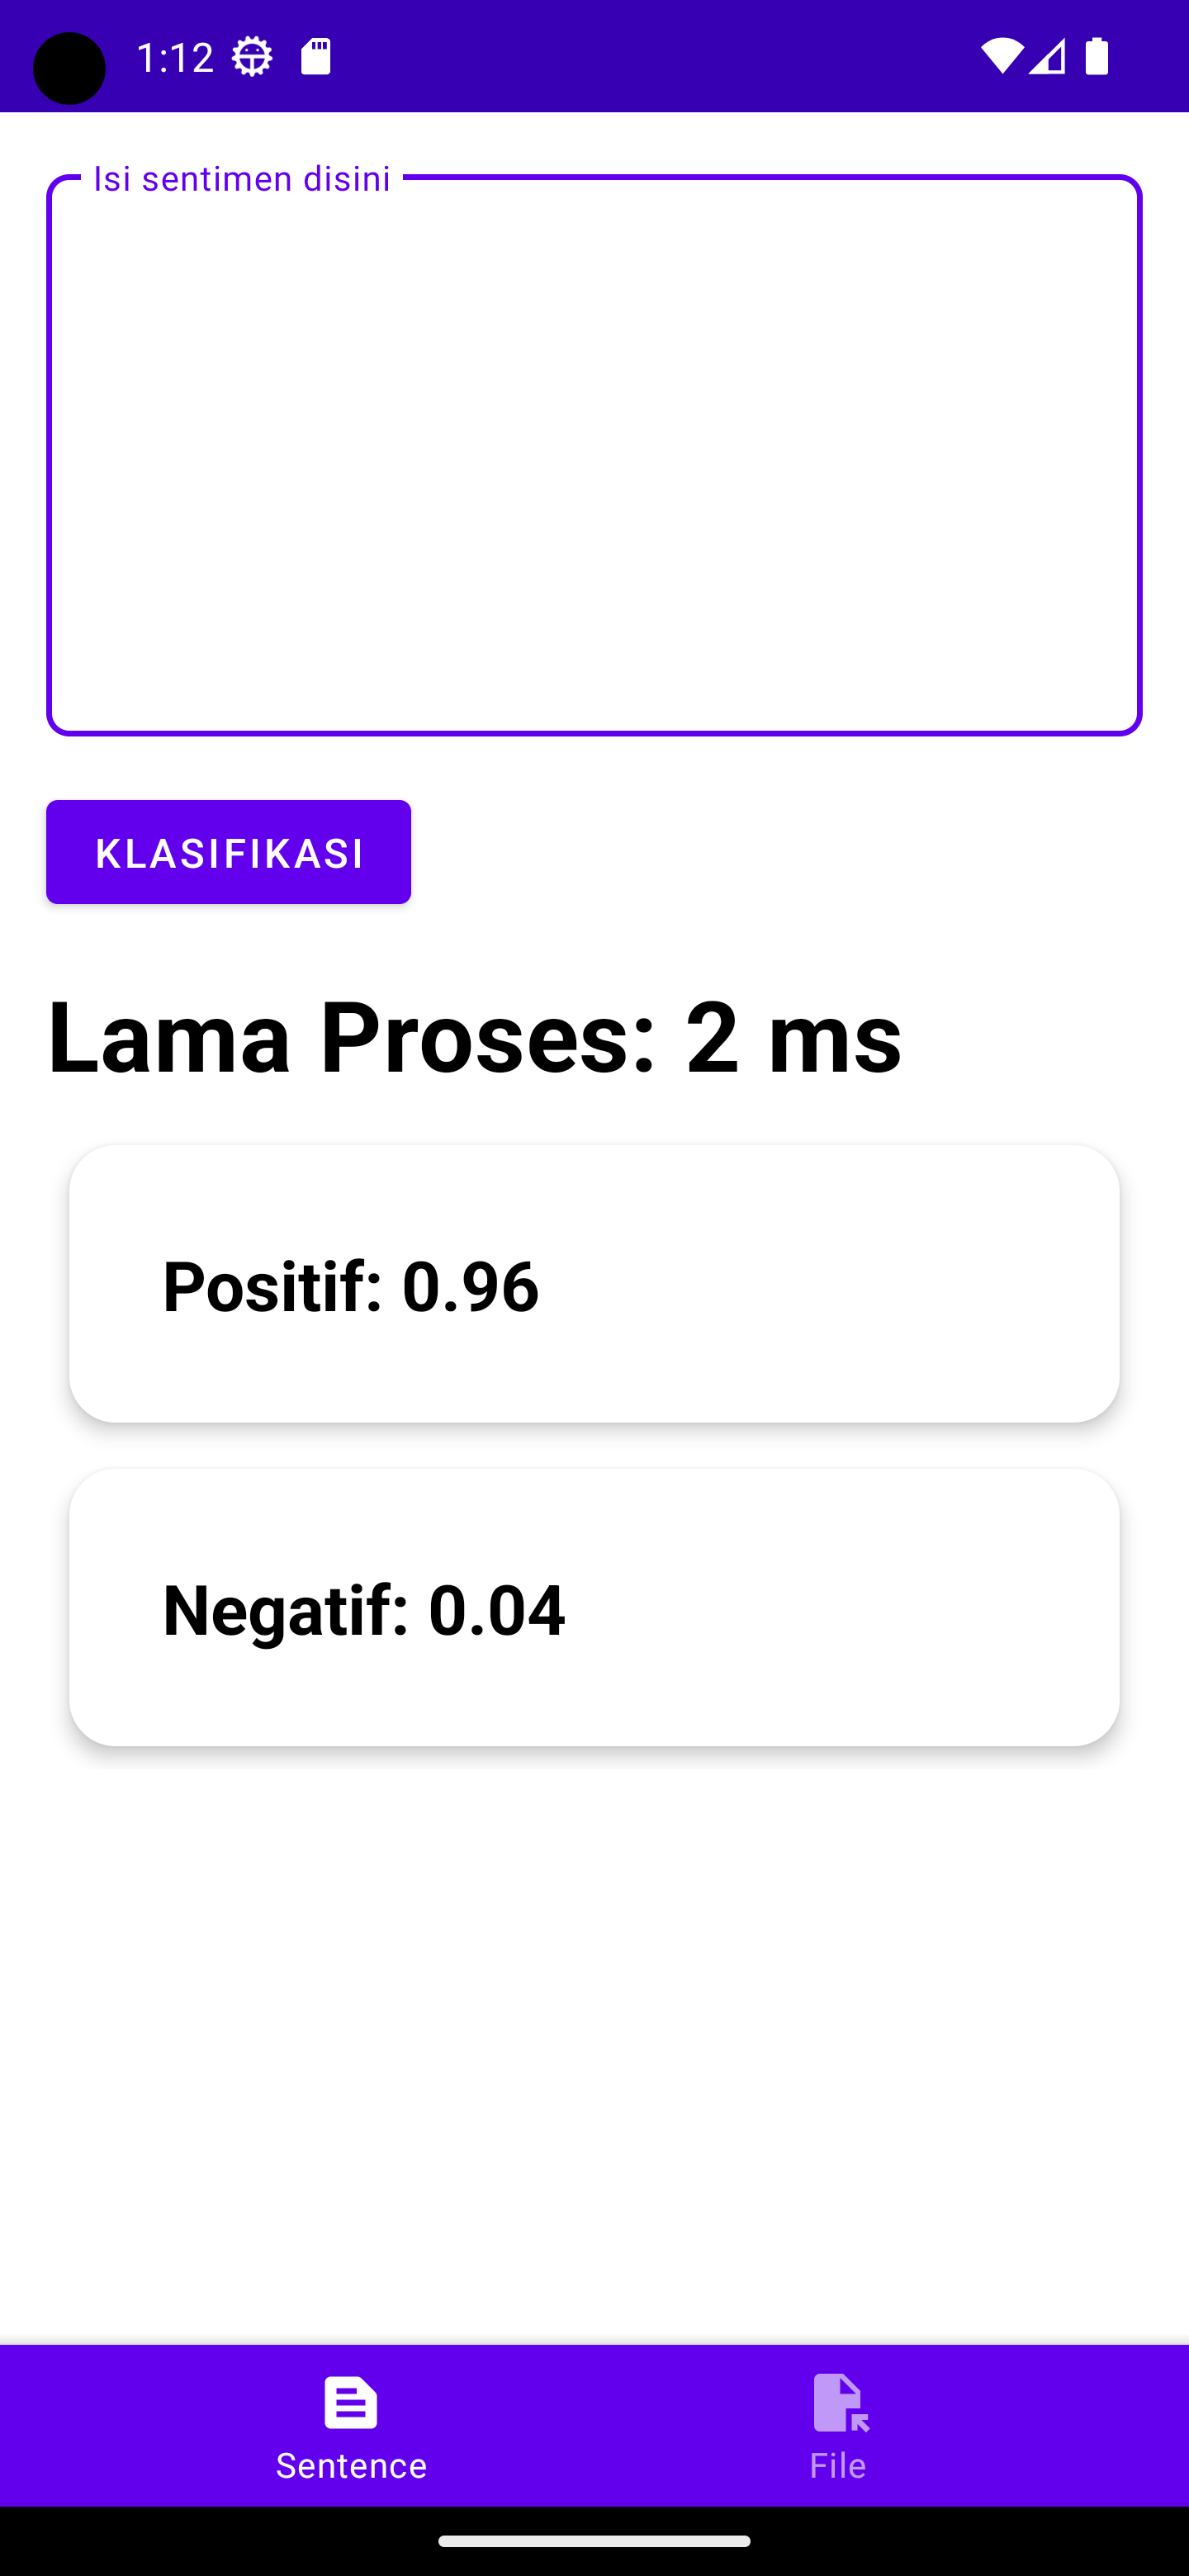
\includegraphics[width=8cm, height=9cm, keepaspectratio]{assets/interface_kalimat.png}}
  \caption{Implementasi Antarmuka Kalimat}
  \label{fig:interface_kalimat}
\end{figure}

\begin{figure}[H]
  \centering
  \fbox{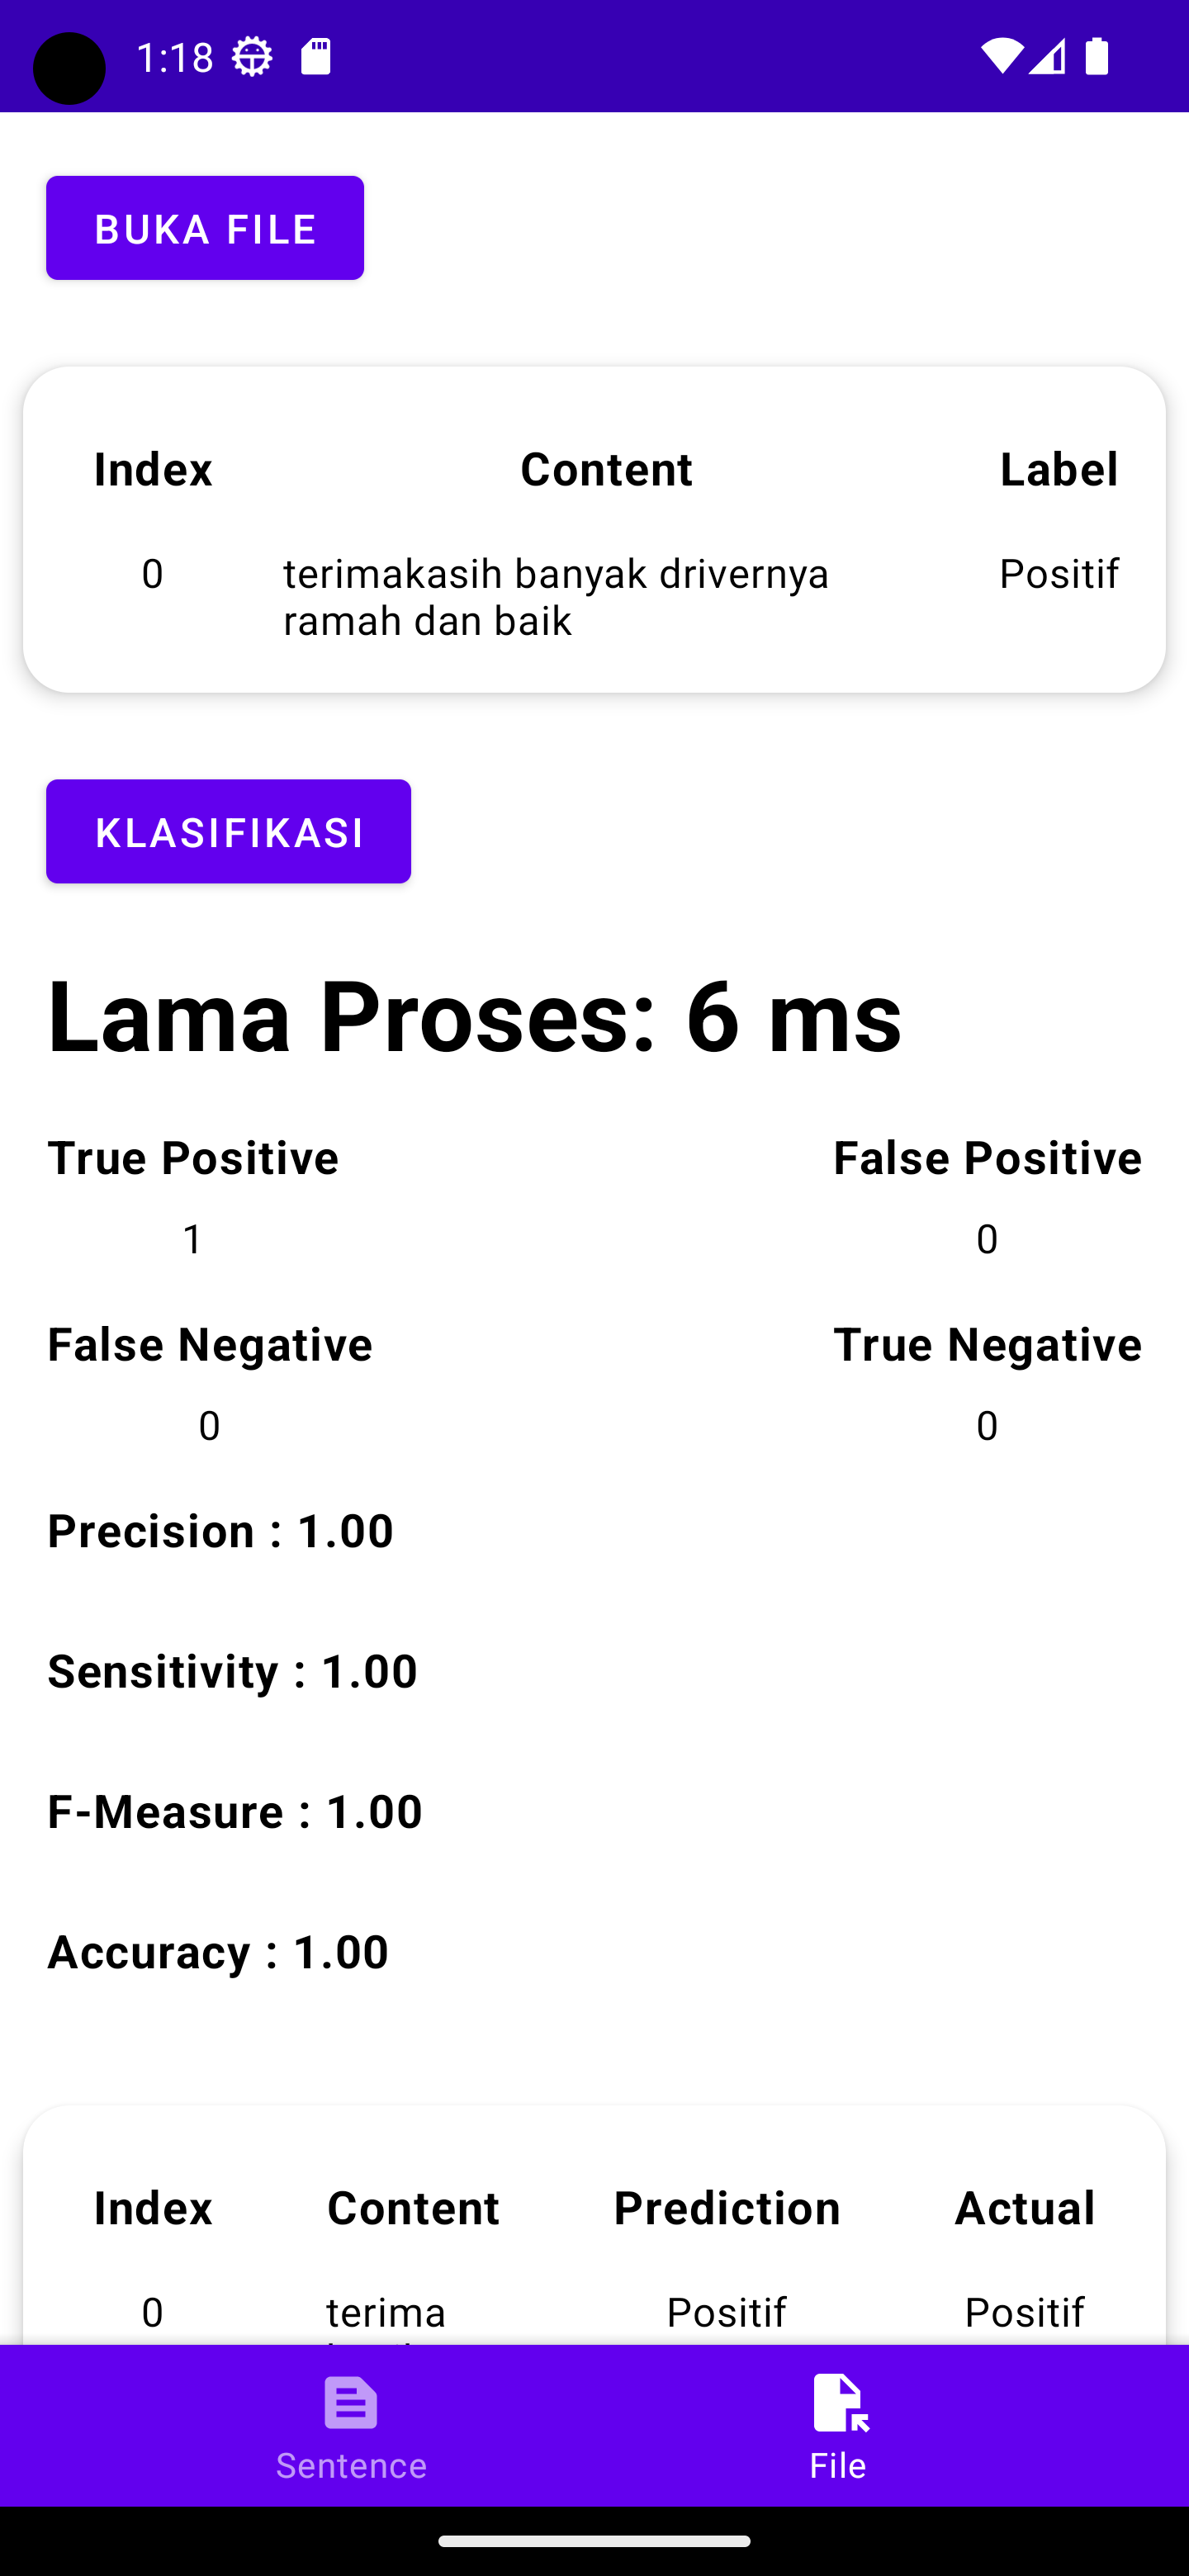
\includegraphics[width=8cm, height=9cm, keepaspectratio]{assets/interface_file.png}}
  \caption{Implementasi Antarmuka File}
  \label{fig:interface_file}
\end{figure}

\section{Fase Transisi}
Fase transisi merupakan fase terakhir dari metode pengembangan perangkat lunak RUP\@. Dalam fase perangkat
lunak diuji berdasarkan proses rencana pengujian untuk memastikan bahwa perangkat lunak dapat digunakan
sesuai dengan ekspektasi pengguna.

\subsection{Pemodelan Bisnis}
Dalam tahapan ini pengujian dilakukan dengan menggunakan cara \emph{black box testing} untuk menguji
apakah perangkat lunak yang dikembangkan berfungsi seperti yang diharapkan.

\emph{Black box testing} adalah cara pengujian dimana penguji tidak mengetahui bagaimana cara suatu sistem
bekerja, namun penguji hanya mengetahui masukan dan keluaran. Tujuan dari \emph{black box testing}
adalah untuk menguji fungsionalitas dari perangkat lunak apakah sudah sesuai dengan perencanaan yang telah dibuat
dan sudah sesuai dengan ekspektasi.

\subsection{Rencana Pengujian}
Rencana pengujian perangkat lunak dideskripsikan pada Tabel~\ref{tab:rencana_pengujian}

\begin{table}[H]
  \centering
  \caption{Rencana Pengujian}
  \label{tab:rencana_pengujian}
  \begin{tabularx}{\textwidth}{|l|X|X|X|c|}
    \hline
    No & \makecell[c]{Skenario                                                                                                                                                                                                                                     \\Pengujian} & \makecell[c]{Hasil yang\\Diharapkan} & \makecell[c]{Hasil\\Pengujian} & \makecell[c]{Kesimpulan} \\ \hline
    1  & Menekan tombol klasifikasi saat sudah menginput kalimat & Sistem menampilkan hasil klasifikasi berupa label dan probabilitasnya                      & Sistem menampilkan hasil klasifikasi berupa label dan probabilitasnya                      & Valid \\ \hline
    2  & Menekan tombol klasifikasi saat sudah membuka file~.csv & Sistem menampilkan hasil klasifikasi berupa index, kalimat, label dan label hasil prediksi & Sistem menampilkan hasil klasifikasi berupa index, kalimat, label dan label hasil prediksi & Valid \\ \hline
  \end{tabularx}
\end{table}

\section{Kesimpulan}
Pada bab ini telah dibahas tahapan yang dilakukan pada pengembangan perangkat lunak menggunakan metode
RUP untuk mengembangkan perangkat lunak yang digunakan sebagai alat bantu untuk melakukan penelitian.
\pagestyle{fancy}
\fancypagestyle{plain}{}
\cfoot{\Roman{chapter}-\arabic{page}}
\rhead{}
\setcounter{page}{1}
\chapter{HASIL DAN ANALISA PENELITIAN}

\section{Pendahuluan}
Dalam bab ini akan membahas tentang hasil dan analisis dari perangkat lunak analisis sentimen
pada angkutan online menggunakan metode CNN yang telah dibuat pada Bab IV. Hasil data uji ditampilkan
dalam bentuk \emph{confusion matrix} dan tabel laporan hasil klasifikasi pada
Tabel~\ref{tab:format_laporan_hasil_klasifikasi}.


\section{Hasil Penelitian}

\subsection{Konfigurasi Percobaan}
Dalam tahapan ini pengujian dilakukan dengan menggunakan data uji yang telah disiapkan sebanyak 1200
\emph{review} yang terdiri dari 600 label positif dan 600 negatif dan data validasi sebanyak 1200
yang terdiri dari 600 label positif dan 600 label negatif. Pengujian dilakukan sesuai dengan kerangka
kerja penelitian. Hasil penelitian dari pengujian yang dilakukan ditampilkan dalam bentuk berupa
\emph{confusion matrix}, nilai \emph{accuracy}, \emph{precision}, \emph{sensitivity (recall)}, dan
\emph{f-measure (f1-score)}.

Optimasi \emph{parameter} atau \emph{fine-tuning} dilakukan dengan menggunakan data latih dan di
validasi dengan menggunakan data validasi berjumlah 1200 \emph{review} dengan 600 label positif dan 600
label negatif. Pada Tabel~\ref{tab:config_fine_tuning} dapat dilihat parameter dan nilai parameter
yang digunakan untuk mendapatkan parameter model CNN terbaik.

\begin{table}[H]
  \centering
  \caption{Konfigurasi Parameter}
  \label{tab:config_fine_tuning}
  \begin{tabularx}{\columnwidth}{|l|l|}
    \hline
    Parameter            & Nilai                          \\ \hline
    epoch                & 125, 150, 175, 200             \\ \hline
    batch\_size          & 8, 16, 32                      \\ \hline
    activation\_function & softmax, sigmoid               \\ \hline
    loss                 & categorical\_crossentropy, mse \\ \hline
  \end{tabularx}
\end{table} \newpage

\pagestyle{fancy}
\fancypagestyle{plain}{}
\rhead{\Roman{chapter}-\arabic{page}}
\cfoot{}

Berdasarkan konfigurasi parameter pada Tabel~\ref{tab:config_fine_tuning} maka dihasilkan skenario percobaan
yang dapat dilihat pada Tabel~\ref{tab:scenario_fine_tuning}. Semua skenario dari \emph{fine-tuning} dilakukan
dengan menggunakan optimizer = adam, learning\_rate = 0.00001, convolution\_activation = relu,
dan word2vec\_trainable = false.

\begin{longtable}[c]{|l|l|l|l|l|}
  \caption{Skenario Fine-Tuning}
  \label{tab:scenario_fine_tuning}                                                  \\
  \hline
  skenario & epoch & batch\_size & activation\_function & loss                      \\ \hline
  %
  \endhead
  %
  1        & 125   & 8           & softmax              & categorical\_crossentropy \\ \hline
  2        & 150   & 8           & softmax              & categorical\_crossentropy \\ \hline
  3        & 175   & 8           & softmax              & categorical\_crossentropy \\ \hline
  4        & 200   & 8           & softmax              & categorical\_crossentropy \\ \hline
  5        & 125   & 16          & softmax              & categorical\_crossentropy \\ \hline
  6        & 150   & 16          & softmax              & categorical\_crossentropy \\ \hline
  7        & 175   & 16          & softmax              & categorical\_crossentropy \\ \hline
  8        & 200   & 16          & softmax              & categorical\_crossentropy \\ \hline
  9        & 125   & 32          & softmax              & categorical\_crossentropy \\ \hline
  10       & 150   & 32          & softmax              & categorical\_crossentropy \\ \hline
  11       & 175   & 32          & softmax              & categorical\_crossentropy \\ \hline
  12       & 200   & 32          & softmax              & categorical\_crossentropy \\ \hline
  13       & 125   & 8           & sigmoid              & mse                       \\ \hline
  14       & 150   & 8           & sigmoid              & mse                       \\ \hline
  15       & 175   & 8           & sigmoid              & mse                       \\ \hline
  16       & 200   & 8           & sigmoid              & mse                       \\ \hline
  17       & 125   & 16          & sigmoid              & mse                       \\ \hline
  18       & 150   & 16          & sigmoid              & mse                       \\ \hline
  19       & 175   & 16          & sigmoid              & mse                       \\ \hline
  20       & 200   & 16          & sigmoid              & mse                       \\ \hline
  21       & 125   & 32          & sigmoid              & mse                       \\ \hline
  22       & 150   & 32          & sigmoid              & mse                       \\ \hline
  23       & 175   & 32          & sigmoid              & mse                       \\ \hline
  24       & 200   & 32          & sigmoid              & mse                       \\ \hline
\end{longtable}

\subsection{Hasil Percobaan}
Hasil pelatihan dari skenario pada Tabel~\ref{tab:scenario_fine_tuning} dapat dilihat pada
Tabel~\ref{tab:result_training_scenario} dan untuk hasil dari prediksi model yang telah dilatih dengan
menggunakan data uji dapat dilihat pada Tabel~\ref{tab:result_testing_scenario}.

\begin{longtable}[c]{|l|l|l|l|l|}
  \caption{Hasil Skenario Pada Pelatihan}
  \label{tab:result_training_scenario}                                 \\
  \hline
  skenario & train\_accuracy & train\_loss & val\_accuracy & val\_loss \\ \hline
  %
  \endhead
  %
  1        & 99,61\%         & 1,28\%      & 89,50\%       & 29,55\%   \\ \hline
  2        & 99,81\%         & 0,57\%      & 89,25\%       & 29,35\%   \\ \hline
  3        & 99,86\%         & 0,53\%      & 89,75\%       & 28,43\%   \\ \hline
  4        & 99,83\%         & 0,56\%      & 88,58\%       & 29,50\%   \\ \hline
  5        & 98,86\%         & 3,97\%      & 89,33\%       & 29,50\%   \\ \hline
  6        & 99,53\%         & 1,81\%      & 89,42\%       & 28,90\%   \\ \hline
  7        & 99,64\%         & 1,29\%      & 89,50\%       & 29,49\%   \\ \hline
  8        & 99,64\%         & 1,03\%      & 88,67\%       & 29,72\%   \\ \hline
  9        & 96,89\%         & 9,39\%      & 88,83\%       & 29,45\%   \\ \hline
  10       & 98,50\%         & 5,38\%      & 89,08\%       & 29,62\%   \\ \hline
  11       & 98,94\%         & 3,57\%      & 89,25\%       & 29,45\%   \\ \hline
  12       & 99,39\%         & 2,43\%      & 88,33\%       & 30,51\%   \\ \hline
  13       & 99,03\%         & 1,05\%      & 89,17\%       & 8,68\%    \\ \hline
  14       & 99,28\%         & 0,80\%      & 89,25\%       & 8,53\%    \\ \hline
  15       & 99,25\%         & 0,08\%      & 89,33\%       & 8,74\%    \\ \hline
  16       & 99,44\%         & 0,06\%      & 89,17\%       & 8,50\%    \\ \hline
  17       & 97,94\%         & 2,05\%      & 89,00\%       & 8,58\%    \\ \hline
  18       & 98,53\%         & 1,52\%      & 89,17\%       & 8,48\%    \\ \hline
  19       & 99,17\%         & 0,09\%      & 89,50\%       & 8,64\%    \\ \hline
  20       & 99,03\%         & 0,09\%      & 88,92\%       & 8,74\%    \\ \hline
  21       & 96,58\%         & 3,48\%      & 88,75\%       & 8,95\%    \\ \hline
  22       & 97,61\%         & 2,47\%      & 88,92\%       & 8,71\%    \\ \hline
  23       & 98,28\%         & 1,77\%      & 89,08\%       & 8,54\%    \\ \hline
  24       & 98,22\%         & 1,70\%      & 88,92\%       & 8,66\%    \\ \hline
\end{longtable}

\begin{longtable}[c]{|l|l|l|l|l|}
  \caption{Hasil Skenario Pada Prediksi Model}
  \label{tab:result_testing_scenario}                  \\
  \hline
  skenario & accuracy & precision & recall  & f1-score \\ \hline
  %
  \endhead
  %
  1        & 90,75\%  & 90,75\%   & 90,75\% & 90,75\%  \\ \hline
  2        & 91,17\%  & 91,18\%   & 91,17\% & 91,17\%  \\ \hline
  3        & 91,42\%  & 91,53\%   & 91,42\% & 91,41\%  \\ \hline
  4        & 91,17\%  & 91,27\%   & 91,17\% & 91,16\%  \\ \hline
  5        & 91,33\%  & 91,35\%   & 91,33\% & 91,33\%  \\ \hline
  6        & 91,33\%  & 91,33\%   & 91,33\% & 91,33\%  \\ \hline
  7        & 91,92\%  & 91,97\%   & 91,92\% & 91,91\%  \\ \hline
  8        & 90,84\%  & 90,83\%   & 90,83\% & 90,83\%  \\ \hline
  9        & 89,58\%  & 89,65\%   & 89,58\% & 89,58\%  \\ \hline
  10       & 90,75\%  & 90,77\%   & 90,75\% & 90,75\%  \\ \hline
  11       & 90,67\%  & 90,68\%   & 90,67\% & 90,67\%  \\ \hline
  12       & 89,83\%  & 89,84\%   & 89,83\% & 89,83\%  \\ \hline
  13       & 91,25\%  & 91,31\%   & 91,25\% & 91,25\%  \\ \hline
  14       & 91,00\%  & 91,10\%   & 91,00\% & 90,99\%  \\ \hline
  15       & 90,33\%  & 90,64\%   & 90,33\% & 90,32\%  \\ \hline
  16       & 90,42\%  & 90,48\%   & 90,42\% & 90,41\%  \\ \hline
  17       & 90,75\%  & 90,92\%   & 90,75\% & 90,74\%  \\ \hline
  18       & 90,83\%  & 90,91\%   & 90,83\% & 90,83\%  \\ \hline
  19       & 91,08\%  & 91,17\%   & 91,08\% & 91,08\%  \\ \hline
  20       & 90,50\%  & 90,51\%   & 90,50\% & 90,50\%  \\ \hline
  21       & 90,08\%  & 90,27\%   & 90,08\% & 90,07\%  \\ \hline
  22       & 90,42\%  & 90,59\%   & 90,42\% & 90,41\%  \\ \hline
  23       & 90,83\%  & 90,90\%   & 90,83\% & 90,83\%  \\ \hline
  24       & 90,75\%  & 90,85\%   & 90,75\% & 90,74\%  \\ \hline
\end{longtable}

Berdasarkan hasil dari skenario pada Tabel~\ref{tab:result_training_scenario} dan
Tabel~\ref{tab:result_testing_scenario} skenario parameter terbaik adalah skenario 13 dengan
parameter epoch = 125, batch\_size = 8, activation = sigmoid, loss = mse dikarenakan di skenario 13
menghasilkan validasi akurasi dengan nilai 89,17\% dan validasi \emph{loss} dengan nilai 8,68\%,
dan menghasilkan nilai \emph{accuracy}, \emph{precision}, \emph{recall}, \emph{f1-score} pada data uji
dengan nilai berturut-turut 91,25\%, 91,31\%, 91,25\%, dan 91,25\%. Oleh karena itu skenario 13 adalah
nilai parameter yang dipakai.

\begin{figure}[H]
  \centering
  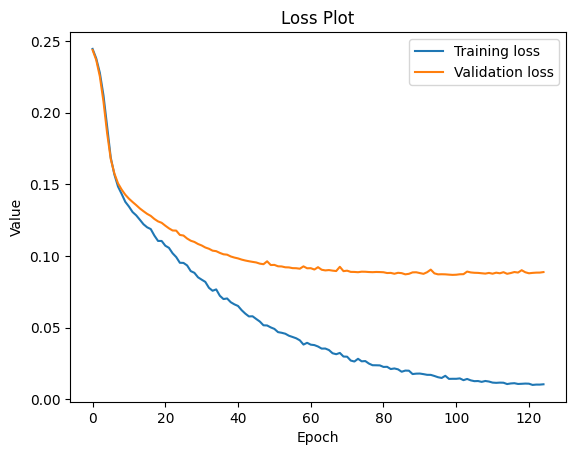
\includegraphics[scale=0.59]{assets/train_validation_loss.png}
  \caption{Train dan Validation Loss Curve}
  \label{fig:train_val_loss_cnn}
\end{figure}

\begin{figure}[H]
  \centering
  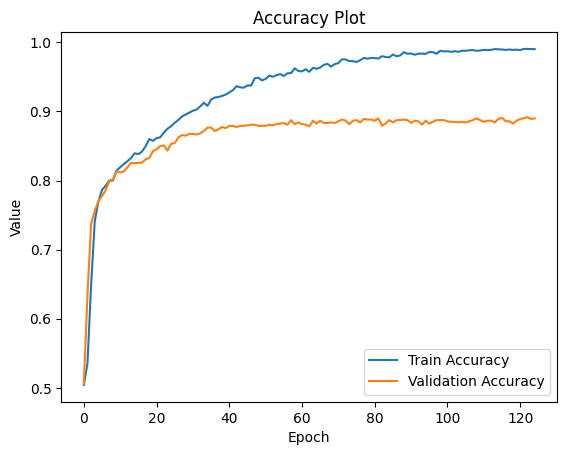
\includegraphics[scale=0.65]{assets/train_validation_accuracy.png}
  \caption{Train dan Validation Accuracy Curve}
  \label{fig:train_val_accuracy_cnn}
\end{figure}

Pelatihan model dilakukan dengan data latih dengan jumlah 3600 yang terdiri dari 1800 positif, dan 1800
negatif, data validasi dengan jumlah 1200 yang terdiri dari 600 positif dan 600 negatif, dan diuji menggunakan
data uji dengan jumlah 1200 yang terdiri dari 600 positif dan 600 negatif. Hasil proses dan kinerja dari
pelatihan model dapat dilihat pada Gambar~\ref{fig:train_val_accuracy_cnn} dan pada Gambar~\ref{fig:train_val_loss_cnn}.

\begin{figure}[H]
  \centering
  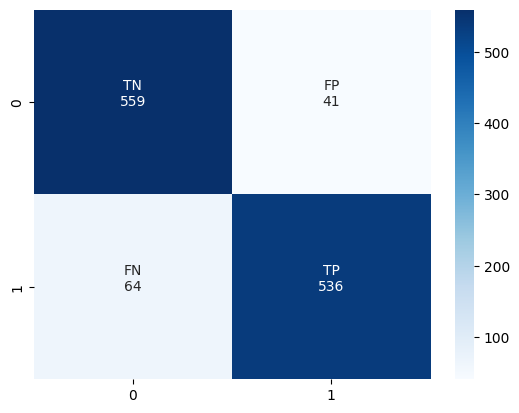
\includegraphics[scale=0.8]{assets/cm_heatmap.png}
  \caption{Confusion Matrix pada Data Uji}
  \label{fig:result_cm_testing}
\end{figure}

\begin{table}[H]
  \centering
  \caption{Laporan Hasil Klasifikasi}
  \label{tab:laporan_hasil_klasifikasi}
  \begin{tabular}{|lllll|}
    \hline
    \multicolumn{1}{|l|}{Label}             & \multicolumn{1}{l|}{\textit{Precision}} & \multicolumn{1}{l|}{\textit{Sensitivity}} & \multicolumn{1}{l|}{\textit{F-Measure}} & Jumlah \\ \hline
    \multicolumn{1}{|l|}{Positif}           & \multicolumn{1}{l|}{92,89\%}            & \multicolumn{1}{l|}{89,33\%}              & \multicolumn{1}{l|}{91,08\%}            & 600    \\ \hline
    \multicolumn{1}{|l|}{Negatif}           & \multicolumn{1}{l|}{89,73\%}            & \multicolumn{1}{l|}{93,17\%}              & \multicolumn{1}{l|}{91,41\%}            & 600    \\ \hline
    \multicolumn{5}{|l|}{}                                                                                                                                                           \\ \hline
    \multicolumn{1}{|l|}{Rata-Rata}         & \multicolumn{1}{l|}{91,31\%}            & \multicolumn{1}{l|}{91,25\%}              & \multicolumn{1}{l|}{91,25\%}            & 1200   \\ \hline
    \multicolumn{1}{|l|}{\textit{Accuracy}} & \multicolumn{3}{l|}{91,25\%}            & 1200                                                                                         \\ \hline
  \end{tabular}
\end{table}

Berdasarkan Tabel~\ref{tab:laporan_hasil_klasifikasi} dan Gambar~\ref{fig:result_cm_testing} kinerja
pada model yang dilakukan pengujian dengan data uji menghasilkan \emph{accuracy}, \emph{precision},
\emph{recall}, \emph{f1-score} dengan nilai berturut-turut 91,25\%, 91,31\%, 91,25\%, dan 91,25\%.
Contoh satu \emph{review} yang bernilai \emph{false positive} dan contoh satu \emph{review} bernilai \emph{false negative}
dapat dilihat pada Tabel~\ref{tab:sample_result_cm_testing}.

\begin{table}[H]
  \centering
  \caption{Sampel Data Uji yang Diklasifikasi}
  \label{tab:sample_result_cm_testing}
  \begin{tabularx}{\columnwidth}{|l|X|l|l|l|}
    \hline
    index & review                                                                                                                       & label   & prediksi & hasil          \\ \hline
    1     & Aplikasi kok gak jelas banget..ternyata masih nyaman di ijo aja lah..                                                        & negatif & positif  & False Positive \\ \hline
    2     & Langsung dapat orderan , tapi tidak ada driver yang datang ke resto , terus bagaimana ini, kasihan pelanggan nungguin. Sudah & positif & negatif  & False Negative \\ \hline
  \end{tabularx}
\end{table}
\newpage

Pada Tabel~\ref{tab:sample_result_cm_testing} dapat dilihat hasil dari klasifikasi terjadi karena kesalahan
model dalam memprediksi kalimat bersifat negatif atau positif. Untuk mengetahui penyebab dari kesalahan prediksi
dari model dapat dilakukan dengan cara melihat hasil praproses dan \emph{surrounding words} dari word2vec yang dapat dilihat
pada Tabel~\ref{tab:analysis_preprocess_predicted_test} dan Tabel~\ref{tab:analysis_mostsimilar_word2vec}.

\begin{table}[H]
  \centering
  \caption{Hasil Praproses Sampel Data Uji}
  \label{tab:analysis_preprocess_predicted_test}
  \begin{tabularx}{\columnwidth}{|l|X|X|}
    \hline
    index & review                                                                                                                       & preprocessed                                    \\ \hline
    1     & Aplikasi kok gak jelas banget..ternyata masih nyaman di ijo aja lah..                                                        & aplikasi tidak banget nyaman ijo                \\ \hline
    2     & Langsung dapat orderan , tapi tidak ada driver yang datang ke resto , terus bagaimana ini, kasihan pelanggan nungguin. Sudah & order tidak driver resto kasihan langgan tunggu \\ \hline
  \end{tabularx}
\end{table}

\begin{longtable}[c]{|l|l|l|l|}
  \caption{Surrounding Words Word2Vec}
  \label{tab:analysis_mostsimilar_word2vec}                                                                                                                                                              \\
  \hline
  preprocessed                                                                                                             & kata                         & serupa                   & nilai\_keserupaan \\ \hline
  \endhead
  \hline
  \endfoot
  %
  \multirow[t]{20}{*}{\begin{tabular}[t]{@{}l@{}}aplikasi\\ tidak\\ banget\\ nyaman\\ ijo\end{tabular}}                    & \multirow[t]{5}{*}{aplikasi} & browser                  & 72,91\%           \\ \cline{3-4}
                                                                                                                           &                              & plugin                   & 70,62\%           \\ \cline{3-4}
                                                                                                                           &                              & Aplikasi                 & 70,45\%           \\ \cline{3-4}
                                                                                                                           &                              & software                 & 69,59\%           \\ \cline{3-4}
                                                                                                                           &                              & server                   & 68,51\%           \\ \cline{2-4}
                                                                                                                           & \multirow[t]{5}{*}{banget}   & aja                      & 74,33\%           \\ \cline{3-4}
                                                                                                                           &                              & bikin                    & 73,77\%           \\ \cline{3-4}
                                                                                                                           &                              & nggak                    & 72,35\%           \\ \cline{3-4}
                                                                                                                           &                              & temen                    & 71,89\%           \\ \cline{3-4}
                                                                                                                           &                              & udah                     & 71,65\%           \\ \cline{2-4}
                                                                                                                           & \multirow[t]{5}{*}{nyaman}   & aman                     & 64,90\%           \\ \cline{3-4}
                                                                                                                           &                              & menyenangkan             & 62,45\%           \\ \cline{3-4}
                                                                                                                           &                              & betah                    & 61,68\%           \\ \cline{3-4}
                                                                                                                           &                              & kondusif                 & 60,52\%           \\ \cline{3-4}
                                                                                                                           &                              & santai                   & 60,46\%           \\ \cline{2-4}
                                                                                                                           & \multirow[t]{5}{*}{ijo}      & laos                     & 74,89\%           \\ \cline{3-4}
                                                                                                                           &                              & Jw                       & 74,42\%           \\ \cline{3-4}
                                                                                                                           &                              & jenang                   & 74,28\%           \\ \cline{3-4}
                                                                                                                           &                              & Lobak                    & 73,92\%           \\ \cline{3-4}
                                                                                                                           &                              & Buncis                   & 73,01\%           \\ \hline
  \multirow[t]{30}{*}{\begin{tabular}[t]{@{}l@{}}order\\ tidak\\ driver\\ resto\\ kasihan\\ langgan\\ tunggu\end{tabular}} & \multirow[t]{5}{*}{order}    & pre                      & 67,55\%           \\ \cline{3-4}
                                                                                                                           &                              & cost                     & 63,24\%           \\ \cline{3-4}
                                                                                                                           &                              & experience               & 61,95\%           \\ \cline{3-4}
                                                                                                                           &                              & challenge                & 61,68\%           \\ \cline{3-4}
                                                                                                                           &                              & job                      & 61,64\%           \\ \cline{2-4}
                                                                                                                           & \multirow[t]{5}{*}{tidak}    & tak                      & 79,03\%           \\ \cline{3-4}
                                                                                                                           &                              & belum                    & 66,92\%           \\ \cline{3-4}
                                                                                                                           &                              & tidaklah                 & 65,90\%           \\ \cline{3-4}
                                                                                                                           &                              & tanpa                    & 60,89\%           \\ \cline{3-4}
                                                                                                                           &                              & jika                     & 54,86\%           \\ \cline{2-4}
                                                                                                                           & \multirow[t]{5}{*}{driver}   & device                   & 66,25\%           \\ \cline{3-4}
                                                                                                                           &                              & client                   & 62,57\%           \\ \cline{3-4}
                                                                                                                           &                              & engine                   & 61,95\%           \\ \cline{3-4}
                                                                                                                           &                              & windows                  & 61,37\%           \\ \cline{3-4}
                                                                                                                           &                              & test                     & 61,12\%           \\ \cline{2-4}
                                                                                                                           & \multirow[t]{5}{*}{resto}    & restaurant               & 66,01\%           \\ \cline{3-4}
                                                                                                                           &                              & cafe                     & 65,77\%           \\ \cline{3-4}
                                                                                                                           &                              & caf\textbackslash{}u00e9 & 61,92\%           \\ \cline{3-4}
                                                                                                                           &                              & restoran                 & 60,86\%           \\ \cline{3-4}
                                                                                                                           &                              & kafe                     & 60,75\%           \\ \cline{2-4}
                                                                                                                           & \multirow[t]{5}{*}{kasihan}  & kasihannya               & 76,93\%           \\ \cline{3-4}
                                                                                                                           &                              & kasihnya                 & 73,59\%           \\ \cline{3-4}
                                                                                                                           &                              & kasih                    & 61,90\%           \\ \cline{3-4}
                                                                                                                           &                              & dengki                   & 56,38\%           \\ \cline{3-4}
                                                                                                                           &                              & penyesalan               & 56,34\%           \\ \cline{2-4}
                                                                                                                           & \multirow[t]{5}{*}{tunggu}   & ditunggu                 & 58,61\%           \\ \cline{3-4}
                                                                                                                           &                              & PPKA                     & 56,31\%           \\ \cline{3-4}
                                                                                                                           &                              & tunggunya                & 50,91\%           \\ \cline{3-4}
                                                                                                                           &                              & Tunggu                   & 49,32\%           \\ \cline{3-4}
                                                                                                                           &                              & keberangkatan            & 49,23\%           \\ \hline
\end{longtable}

Berdasarkan Tabel~\ref{tab:analysis_preprocess_predicted_test} dan Tabel~\ref{tab:analysis_mostsimilar_word2vec}
pada index ke-1 hasil praproses terdapat kata `banget' dan `nyaman' yang memiliki \emph{surrounding word}
yang memiliki makna positif maka model memprediksi kalimat memiliki label positif, sedangkan untuk
di index ke-2 terdapat kata `tidak', `kasihan', dan `tunggu' yang memiliki \emph{surrounding words}
yang memiliki makna negatif maka model memprediksi kalimat memiliki label negatif.


\section{Kesimpulan}
Kesimpulan dari pengujian model pada data uji yang telah dilakukan adalah parameter yang menghasilkan
kinerja model terbaik terdapat pada skenario 20 dengan nilai parameter epoch = 125, batch\_size = 8 dan
word2vec\_trainable = false, activation = sigmoid, optimizer = adam, learning\_rate = 0.00001,
convolution\_activation = relu, dan loss = mse yang menghasilkan nilai \emph{accuracy},
\emph{precision}, \emph{recall}, dan \emph{f1-score} berturut-turut 91,25\%, 91,31\%, 91,25\%, dan 91,25\%.
\pagestyle{fancy}
\fancypagestyle{plain}{}
\cfoot{\Roman{chapter}-\arabic{page}}
\rhead{}
\setcounter{page}{1}
\chapter{KESIMPULAN DAN SARAN}

\section{Kesimpulan}
Kesimpulan yang dapat diambil sebagai hasil dari penelitian ini adalah sebagai berikut:
\begin{enumerate}
  \item Perangkat lunak analisis sentimen pada opini publik tentang angkutan online dengan menggunakan
        metode CNN berbasis \emph{mobile} dapat dikembangkan dengan baik.
  \item Analisis sentimen dengan menggunakan metode CNN dapat menghasilkan nilai akurasi, precision,
        recall, dan f1-score berturut-turut 91,25\%, 91,31\%, 91,25\%, dan 91,25\%. pada data uji dengan pembagian
        data latih, data validasi, dan data uji dengan rasio 60:20:20 dan konfigurasi dengan nilai parameter
        epoch = 125, batch\_size = 8, word2vec\_trainable = false, optimizer = adam, learning\_rate = 0.00001,
        loss = mse, fully\_connected\_activation = sigmoid dan convolution\_activation = relu.
\end{enumerate}

\section{Saran}
Saran yang dapat digunakan dari penulis untuk penelitian lebih lanjut sebagai berikut:
\begin{enumerate}
  \item Menambahkan dataset karena dataset \emph{review} dengan jumlah 6000 tergolong sedikit untuk melatih CNN\@.
  \item Menambahkan metode untuk menormalisasi kata menjadi kata baku. 
  \item Mengubah emoji menjadi kata. 
  \item Mengubah angka menjadi kata.
\end{enumerate}


\pagenumbering{roman}
\cfoot{\roman{page}}
\lhead{}
\rhead{}
\renewcommand\thepage{\roman{page}}

\setcounter{page}{15}
\bibliographystyle{apacite}
\bibliography{ref}

\end{document}
